%\documentclass[letterpaper,10pt]{article}
\documentclass[onecolumn]{emulateapj}





\usepackage{geometry}   % See geometry.pdf to learn the layout
                        % options.  There are lots.
\usepackage[latin1]{inputenc}
\usepackage{graphicx}
\usepackage{epstopdf}
\usepackage{amsmath,amsfonts,amssymb}
\usepackage{soul}

\DeclareGraphicsRule{.tif}{png}{.png}{`convert #1 `dirname #1`/`basename #1 .tif`.png}




%\author{Michael L. Norman\altaffilmark{1,3}}
%\author{Daniel R. Reynolds\altaffilmark{4}}
%\author{Geoffrey C. So\altaffilmark{1}}
%\author{Robert P. Harkness\altaffilmark{2,3}}

%\affiliation{
%\altaffilmark{1}CASS, University of California, San Diego, 9500 Gilman Drive La Jolla, CA 92093-0424\\
%\altaffilmark{2}NICS, Oak Ridge National Laboratory, 1 Bethel Valley Rd, Oak Ridge, TN 37831\\
%\altaffilmark{3}SDSC, University of California, San Diego, 9500 Gilman Drive La Jolla, CA 92093-0505\\ 
%\altaffilmark{4}Southern Methodist University, 6425 Boaz Ln, Dallas, TX 75205\\
%}

\renewcommand{\(}{\left(}
\renewcommand{\)}{\right)}
\newcommand{\vb}{{\bf v}_b}
\newcommand{\xvec}{{\bf x}}
\newcommand{\Omegabar}{\bar{\Omega}}
\newcommand{\rhob}{\rho_b}
\newcommand{\dt}{\Delta t}
\newcommand{\Eot}{E^{OT}}
\newcommand{\Enu}{E_{\nu}}
\newcommand{\Fnu}{{\bf F}_{\nu}}

\newcommand{\Pnu}{\overline{\bf P}_{\nu}}
\newcommand{\Ef}{E_f}
\newcommand{\sighat}{\hat{\sigma}}
\newcommand{\R}{I\!\!R}
\newcommand{\Rthree}{\R^3}
\newcommand{\eh}{e_h}
\newcommand{\ec}{e_c}
\newcommand{\Edd}{\mathcal F}
\newcommand{\Eddnu}{\Edd_{\nu}}
\newcommand{\mn}{{\tt n}}
\newcommand{\mB}{\mathcal B}
\newcommand{\mC}{{\mathcal C}}
\newcommand{\mL}{{\mathcal L}}
\newcommand{\mD}{{\mathcal D}}
\newcommand{\mDnu}{\mD_{\nu}}
\newcommand{\mCnu}{\mC_{\nu}}
\newcommand{\mLnu}{{\mathcal L}_{\nu}}
\newcommand{\mCe}{\mC_e}
\newcommand{\mLe}{\mL_e}
\newcommand{\mCn}{\mC_{\mn}}
\newcommand{\mLn}{\mL_{\mn}}
\newcommand{\chibar}{\bar{\chi}}
\newcommand{\ngammadot}{\dot{N}_{\gamma}}
\newcommand{\hi}{H {\footnotesize I}~}
\newcommand{\hii}{H {\footnotesize II}~}

%\newcommand{\mnras}{Mon. Not. R. Astr. Soc.}
%\newcommand{\araa}{Ann. Rev. Astron. Astrophys.}
%\newcommand{\apj}{Ap. J.}
%\newcommand{\apjs}{Ap. J. Supp.}
%\newcommand{\nat}{Nature}
\newcommand{\na}{New Astron.}
%\newcommand{\physrep}{Phys. Reports}


\setlength{\parindent}{0em}
\setlength{\parskip}{2ex}
\textheight 9truein
\textwidth 6.5truein
\addtolength{\oddsidemargin}{+0.25in}
\addtolength{\evensidemargin}{+0.25in}
\addtolength{\topmargin}{+0.5in}

\begin{document}

%\title{Direct Numerical Simulation of Reionization in Large Cosmological Volumes I: Numerical Methods and Tests}
\title{Fully-Coupled Simulation of Cosmic Reionization. I: Numerical Methods and Tests}

%\author{Michael L. Norman, Daniel R. Reynolds, Geoffrey C. So, Robert P. Harkness}

\author{Michael L. Norman\altaffilmark{1,3}}
\author{Daniel R. Reynolds\altaffilmark{4}}
\author{Geoffrey C. So\altaffilmark{1}}
\author{Robert P. Harkness\altaffilmark{2,3}}
\author{John H. Wise\altaffilmark{5}}

\affiliation{
\altaffilmark{1}CASS, University of California, San Diego, 9500 Gilman Drive La Jolla, CA 92093-0424\\
\altaffilmark{2}NICS, Oak Ridge National Laboratory, 1 Bethel Valley Rd, Oak Ridge, TN 37831\\
\altaffilmark{3}SDSC, University of California, San Diego, 9500 Gilman Drive La Jolla, CA 92093-0505\\ 
\altaffilmark{4}Southern Methodist University, 6425 Boaz Ln, Dallas, TX 75205\\
\altaffilmark{5}Center for Relativistic Astrophysics, Georgia Institute of Technology, 837 State St, Atlanta, GA 30332 \\
}



\begin{abstract}
We describe an extension of the {\em Enzo} code to enable \st{the direct numerical} {\bf fully-coupled radiation hydrodynamical} simulation 
of inhomogeneous reionization in large {\bf $\sim (100 Mpc)^3$} cosmological volumes {\bf with thousands to millions of point sources} . \st{By direct we mean} {\bf We solve}
all dynamical, radiative {\bf transfer, thermal, and ionization processes} \st{and chemical properties} \st{are solved} self-consistently on the same mesh, 
as opposed to a postprocessing approach which coarse-grains the radiative transfer. We do,
however, employ a simple subgrid model for star formation which we calibrate to observations. 
The numerical method presented is a modification of an earlier method presented in Reynolds et al., {\bf differing principally in the operator splitting algorithm we we use to advance the system of equations.} Radiation transport is done in the grey flux-limited diffusion (FLD) approximation, which is solved by
implicit time integration split off from the gas energy and ionization equations, which are solved
separately. This results in 
a faster and more robust scheme for cosmological applications compared to the earlier method. 
The FLD equation is solved
using the {\em hypre} optimally scalable geometric multigrid solver from LLNL. 
By treating the ionizing radiation as a grid field as opposed to rays, our method
is scalable with respect to the number of ionizing sources, limited only by the parallel scaling
properties of the radiation solver. We test the speed and accuracy of our approach on a 
number of standard verification and validation tests.  We show {\bf by direct comparison with {\em Enzo}'s adaptive ray tracing method {\em Moray}} that the well-known 
inability of FLD to cast a shadow behind opaque clouds \st{has little effect on the 
photoevaporation timescale of the cloud, or} {\bf has a minor effect on the evolution of ionized volume and mass fractions}
in a reionization simulation validation test. 
We illustrate \st{its application} {\bf an application of our method} to the
problem of inhomogeneous reionization in a \st{20} {\bf80} Mpc comoving box resolved with
\st{$800^3$} {\bf $3200^3$} Eulerian grid cells and dark matter particles. 
\end{abstract}
\keywords{cosmology: theory -- reionization -- methods: numerical -- radiative transfer}

\maketitle


\section{Introduction}
\label{sec:introduction}

The Epoch of Reionization (EoR) is an active area of research observationally,
theoretically, and computationally. Observations constrain the tail end of hydrogen reionization
to the redshift range $z=6-8$ \citep{RobertsonEtAl2010}. These observations include the presence of Gunn-Peterson
troughs in the Ly $\alpha$ absorption spectra of high redshift quasars \citep{FanEtAl2006}, and 
the strong evolution of Lyman $\alpha$ emitter luminosity function (Robertson et al. 2010 and references
therein.) 
Observations from the WMAP and Planck satellites tell us that the universe was substantially 
ionized by $z \approx 10$ but can say little about the
reionization history or topology \citep{JarosikEtAl2011,Planck2013}. 
High redshift 21cm observations hold forth great promise of elucidating the details of this transition \citep{BarkanaLoeb2007, PritchardLoeb2012}, but these results are still in the future. 

It is believed that early star forming galaxies provided the bulk of the UV photons responsible for
reionization \citep{RobertsonEtAl2010,RobertsonEtAl2013}, but early QSOs may have also contributed \citep{MadauEtAl1999, BoltonHaehnelt2007, HaardtMadau2012}.  The ``galaxy reionizer" hypothesis has been greatly strengthened by the recent advances in the study of high redshift galaxies afforded by the IR-sensitive Wide Field Camera 3 (WFC3) aboard the Hubble Space Telescope \citep[e.g.][]{RobertsonEtAl2010, RobertsonEtAl2013, BouwensEtAl2011, BouwensEtAl2011b, OeschEtAl2013}.  Within uncertainties, the luminosity function of $z=6$ Lyman break galaxies (LBGs) appears to be sufficient to account for reionization at that redshift from a photon counting argument \citep{BoltonHaehnelt2007, RobertsonEtAl2010, BouwensEtAl2012}. Among the observational uncertainties are the faint-end slope of the galaxy luminosity function \citep{WiseCen2009,LabbeEtAl2010,BouwensEtAl2012}, the spectral energy distribution of the stellar population \citep{CowieEtAl2009,WillotEtAl2010,HaardtMadau2012}, and the escape fraction of ionizing photons \citep{WyitheEtAl2010, YajimaEtAl2011, MitraEtAl2013}. Among the theoretical uncertainties are the number of ionizing photons per H atom required to bring the neutral IGM to its highly ionized state by $z=6$, the clumping factor correction to the mean IGM recombination time \citep{PawlikEtAl2009, RaicevicTheuns2011, FinlatorEtAl2012, ShullEtAl2012, RobertsonEtAl2013}, 
and the contribution of Pop III stars and accreting black holes to the early and late stages of reionization \citep{BoltonHaehnelt2007,TracGnedin2011,AhnEtAl2012}. 

When assessing whether an observed population of high-z galaxies is capable of 
reionizing the universe (e.g., Robertson et al. 2013), observers often use the criterion derived
by \cite{MadauEtAl1999} for the ionzing photon volume density $\dot{\mathcal{N}}_{ion}$ necessary
to maintain the clumpy IGM in an ionized state:

\begin{align}
\label{eq:ndot}
\dot{\mathcal{N}}_{ion}(z) &= \frac{\bar{n}_\mathrm{H}(0)}{\bar{t}_{rec}(z)} = (10^{51.2}s^{-1}Mpc^{-3})\left(\frac{C}{30}\right) \notag\\
&\times \left(\frac{1+z}{6}\right)^3 \left(\frac{\Omega_b h_{50}^2}{0.08}\right)^2,
\end{align}

where $\bar{n}_\mathrm{H}(0)$ is the mean comoving number density of H atoms, $C \equiv \langle n^2_\mathrm{H\,II} \rangle /\langle n_\mathrm{H\,II} \rangle ^2$ is the H {\footnotesize II} clumping factor (angle brackets denote volume average over a suitably large volume that the average is globally meaningful),
and the rest of the symbols have their usual meaning. 
The origin of this formula is a simple photon counting argument, which says 
that in order to maintain ionization at a given redshift $z$, 
the number of ionizing photons emitted in
a large volume of the universe multiplied by a characteristic recombination
time, denoted $\bar{t}_{rec}$,  must equal the number of hydrogen atoms: $\dot{\mathcal{N}}_{ion} \times \bar{t}_{rec} = \bar{n}_\mathrm{H}(0)$.
The clumping factor enters as a correction factor to account for the density inhomogeneties in the IGM
induced by structure formation. We note that $\bar{t}_{rec}$ is not the volume average of the local recombination time of the
ionized plasma, as this would heavily weight regions with the {\em longest} recombination
times; i.e. voids. A proper derivation of  Equation \eqref{eq:ndot} shows that $\bar{t}_{rec} \propto \langle t_{rec}^{-1} \rangle ^{-1}$, which weights regions
with the {\em shortest} recombination times; i.e. regions at the mean density and above. 

Equation \eqref{eq:ndot} is based on a number of simplifying assumptions discussed by
\cite{MadauEtAl1999}, including the assumption $\bar{t}_{rec} \ll t$. It is this assumption that allows history-dependent effects to be ignored, and a quasi-instantaneous analysis of the 
photon budget for reionization to be done. The validity of this assumption is naturally
redshift dependent, but it is also dependent upon the adopted definition of $\bar{t}_{rec}$.  A second comment about Equation \eqref{eq:ndot} is that it does not ask how many ionizing photons per H atom are required to convert a neutral IGM to a fully ionized one, only how many are required to {\em maintain} the IGM in an ionized state. Because the recombination time is short at high redshifts, it is expected that this number is greater than one. 

In this paper we examine these and related topics within the context of a direct numerical simulation of cosmic reionization based on a new flux-limited diffusion radiation transport solver installed in the {\em Enzo} code \citep{NormanEtAl2013} (hereafter Paper I).
Our approach self-consistently couples all the relevant physical processes 
(gas dynamics, dark matter dynamics, self-gravity, star formation/feedback, 
radiative transfer, nonequilibrium ionization/recombination, heating and cooling) and evolves the
system of coupled equations on the same high resolution mesh. We refer to this
approach as {\em direct numerical simulation} or {\em resolution matched}, in contrast to previous approaches 
which decouple and coarse-grain the radiative transfer and ionization balance 
calculations relative to the underlying dynamical calculation.
Our method is
scalable with respect to the number of radiation sources, size of the mesh, and the
number of computer processors employed.
This scalability permits us to simulate cosmological reionization in large cosmological
volumes (L $\sim100$ Mpc) while directly modeling the sources and sinks of ionizing 
radiation,  
including radiative feedback effects such as photoevaporation of gas from halos, 
Jeans smoothing of the IGM, and enhanced recombination due to small scale clumping. 
In this the first of several application papers, we investigate in a volume of modest size (L=$20$ Mpc) the mechanics of reionization from stellar sources forming in high-$z$ galaxies, the role of gas clumping, recombinations, and the photon budget required to complete reionization.

By analyzing this simulation we are able to critically examine the validity of  Equation \eqref{eq:ndot} as a predictor of when the end of EoR will occur, and we can calculate the integrated number of ionizing photons 
per H atom needed to ionize the simulated volume $\gamma_{ion}/H=\int dt \dot{\mathcal{N}}_{ion} / \bar{n}_\mathrm{H}(0)$. Ignoring recombinations within the virial radii of collapsed halos, we find $\gamma_{ion}/H \approx 2$. This result
supports the ``photon starved'' reionization scenario discussed by \cite{BoltonHaehnelt2007}.
We also examine whether modern revisions to Equation \eqref{eq:ndot} using alternatively defined 
clumping factors \citep{PawlikEtAl2009, RaicevicTheuns2011, FinlatorEtAl2012, ShullEtAl2012} are 
improvements over the original. We find they systematically overestimate the redshift of reionization completion $z_{reion}$ because the condition $\bar{t}_{rec}/t \ll 1$ is never obeyed.  We study the accuracy and validity of the time-dependent analytic model of \cite{MadauEtAl1999}, and find that while it is in better agreement with the simulation, it also overestimates $z_{reion}$ because it ignores important corrections to the ionization term at early and late times.

This paper is organized as follows: in \S\ref{Method} we discuss the design criteria 
for the simulation and briefly outline the basic equations and implementation of the FLD radiation transport model, referring the
reader to Paper I for a more complete description of the numerical algorithms and tests.  
In \S\ref{GeneralResults},  we present some general features of the simulation and demonstrate its broad consistency with observed star formation rate density and high redshift 
galaxy luminosity function. 
%Because we track the ionization fraction of the gas at every point in the volume as a function of time, a more quantitative language is required to say when the simulated volume is X\% ionized; this is provided in \S\ref{QuantitativeLanguage}. 
%In \S\ref{IOOI} we examine the mechanics of reionization in our simulation, and in particular question whether ``inside-out'' or ``outside-in'' is a better description of certain phases of evolution. 
In \S\ref{sec:ClumpingFactors} we examine the accuracy of different clumping factor approaches to estimating the redshift of complete reionization.
In \S\ref{escape} we derive a global estimate for the circumgalactic absorption of ionizing radiation from our simulation. 
In \S\ref{Qdot} we test a simple analytic model for the evolution of the ionized volume fraction $Q_\mathrm{H\,II}$ and present an improvement to the model which better agrees with our simulation. 
In \S\ref{Discussion} we
discuss implications of our results on the current understanding of
reionization.  And finally, in \S\ref{Conclusions} we end with a
summary of our main results and conclusions.




\section{Mathematical Formulation}
\label{sec:math_formulation}


%Primordial gas chemistry (do we need more detail here?) No, refer to Bryan et al. (2013)

We solve the coupled equations of multispecies gas dynamics, dark matter dynamics, self-gravity, 
primordial gas chemistry, radiative transfer, and gas cooling/heating in a comoving volume
of the expanding universe. In this paper we assume the governing equations are discretized on a cubic uniform Cartesian mesh  in comoving 
coordinates assuming periodic boundary conditions. In Reynolds et
al. (in prep.) we generalize our method to adaptive meshes. 
The background spacetime is assumed to be a FRW model with $\Lambda$CDM cosmological parameters \citep{WMAP7}. In this work we consider only the 5 ionic states of H and He and $e^-$; i.e., the commonly used ``6-species" model of primordial gas \citep{AbelEtAl1997, Anninos97}. Molecular hydrogen chemistry is ignored as we are primarily concerned with the later stages of H reionization driven by star formation in atomic line cooling galaxies. Star formation is modeled phenomenologically through a subgrid model described in the next section. Newly formed stars are sources of UV radiation, and the radiation is transported in the grey flux-limited diffusion approximation. Star formation in spatially distributed galaxies thus sources an inhomogeneous and evolving ionizing radiation field, which is used to calculate the local ionization and thermal state of the gas. This in turn controls the local cooling rate of the gas, and by virtue of the subgrid star formation model, the local star formation rate. We thus have a closed system of equations that we can evolve forward in time subject to the choice of initial conditions. In all but the verification test problems, cosmological initial conditions are generated using standard methods.  

The choice of flux-limited diffusion (FLD) is motivated by its
simplicity and its ability to smoothly transition between optically
thin and thick regimes. Its properties as well as its limitations are
well understood, and efficient numerical methods exist for parallel
computation (e.g., Hayes et al. 2006). A second motivation is that we
are interested in modeling reionization in large cosmological volumes
and field-based solvers scale independently of the number of sources, unlike ray tracing
methods. In the early stages of reionization, when HII regions are
largely isolated, FLD provides accurate I-front speeds, as shown by
our verification tests in Sec. 4.1. At late times, during and after
overlap, the gas is bathed in a diffuse radiation field arising from
numerous point sources for which the angular structure of the
radiation field is unimportant. It is during the early percolation
phase when several HII regions merge that FLD is inaccurate with
regard to the angular distribution of the radiation field. This leads
to some inaccuracies of the shapes of the I-fronts compared to a
solution obtained using ray tracing (see Sec. 4.3). However we
consider these shape differences of secondary importance since we are
interested in globally averaged ionization properties. A well known
limitation of FLD is that opaque blobs do not cast shadows if they are illuminated from one side (e.g.,
Hayes \& Norman 2003). Instead, the radiation flows around the
backside of the irradiated blob. By contrast, a ray tracing method
will cast a sharp shadow (Iliev et al. 2009, Wise \& Abel 2011). What
matters for global reionization simulations however is how long the
opaque blobs remain self-shielded; i.e., their photoevaporation
times. We have compared the photoevaporation times for identically
resolved blobs using FLD and the ray tracing method of Wise \& Abel
(2011), and find them comparable despite the inability of FLD to cast
a shadow (sec Sec.~\ref{subsubsec:test7}). 

{\bf Finally we comment on the use of a {\em grey} treatment of the radiation field. 
Grey FLD is an improvement over monochromatic radiative transfer as it provides a formalism for calculating the contributions of higher energy photons above the ionization threshold to the frequency-integrated photoionization rate and photoheating rate. It is not as accurate as multifrequency/multigroup radiative transfer in that it does not model spectral hardening of the radiation field and preionization ahead of the I-front. At present, no large-scale simulations of cosmological reionization include these effects, which are expected to be small for the soft ionizing spectrum of Pop II stars. }



We consider the coupled system of partial differential equations
\citep{ReynoldsHayesPaschosNorman2009},
\begin{align}
  \label{eq:gravity}
  \nabla^2 \phi &= \frac{4\pi g}{a}(\rhob + \rho_{dm} - \langle \rho \rangle), \\
  \label{eq:cons_mass}
  \partial_t \rhob + \frac1a \vb \cdot \nabla
    \rhob &= -\frac1a \rhob \nabla\cdot\vb - \dot{\rho}_{SF}, \\
  \label{eq:cons_momentum}
  \partial_t \vb + \frac1a\(\vb\cdot\nabla\)\vb &=
    -\frac{\dot{a}}{a}\vb - \frac{1}{a\rhob}\nabla p - \frac1a
    \nabla\phi, \\
  \label{eq:cons_energy}
  \partial_t e + \frac1a\vb\cdot\nabla e &=
    - \frac{2\dot{a}}{a}e
    - \frac{1}{a\rhob}\nabla\cdot\left(p\vb\right) 
    - \frac1a\vb\cdot\nabla\phi + G - \Lambda  + \dot{e}_{SF} \\
  \label{eq:chemical_ionization}
  \partial_t \mn_i + \frac{1}{a}\nabla\cdot\(\mn_i\vb\) &=
    \alpha_{i,j} \mn_e \mn_j - \mn_i \Gamma_{i}^{ph}, \qquad
    i=1,\ldots,N_s \\
  \label{eq:cons_radiation}
  \partial_t E + \frac1a \nabla\cdot\(E \vb\) &= 
    \nabla\cdot\(D\nabla E\) - \frac{\dot{a}}{a}E - c \kappa E + \eta.
\end{align}
The comoving form of Poisson's equation \eqref{eq:gravity} is used to
determine the modified gravitational potential, $\phi$, 
where $g$ is the gravitational constant, $\rhob$ is the comoving
baryonic density, $\rho_{dm}$ is the dark matter density, and 
$\langle \rho \rangle$ is the cosmic mean density.  The collisionless
dark matter density $\rho_{dm}$ is evolved using the Particle-Mesh
method, as described in
\cite{HockneyEastwood1988,NormanBryan1999,OSheaEtAl2004}.  The
conservation equations \eqref{eq:cons_mass}-\eqref{eq:cons_energy}
correspond to the compressible Euler equations in a comoving
coordinate system \cite{BryanEtAl1995}.  These relate the density to
the proper peculiar baryonic velocity $\vb\equiv a(t)\dot{\xvec}$, the
proper pressure $p$, and the total gas energy per unit mass $e$.   
The equations \eqref{eq:chemical_ionization} model
ionizaton processes between the chemical species HI, HII, HeI, HeII,
HeIII and the electron density.  Here, $\mn_i$ denotes the
$i^{th}$ comoving elemental species number density, $\mn_e$ is the
electron number density, $\mn_j$ corresponds to ions that react
with the species $i$, and $\alpha_{i,j}$ are the reaction rate
coefficients defining these interactions
\citep{AbelEtAl1997,HuiGnedin1997}.  The equation
\eqref{eq:cons_radiation} describes the flux-limited diffusion (FLD)  
approximation of radiation transport in a cosmological medium
\citep{HayesNorman2003,Paschos2005}, where $E$ is the comoving grey
radiation energy density.  Within this equation, the function
$D$ is the {\em flux limiter} that depends on face-centered values of
$E$, $\nabla E$ and the opacity $\kappa$ \citep{Morel2000},
\begin{align}
  D &= \min\left\{c \(9\kappa^2 + R^2\)^{-1/2}, D_{max}\right\},\quad\mbox{and}\quad
  R = \max\left\{\frac{|\partial_{x} E|}{E},R_{min}\right\}.
\end{align}
Here the spatial derivative within $R$ is computed using
non-dimensional units at the computational face adjoining two
neighboring finite-volume cells, $D_{max}=0.006\,c\,L_{unit}$ and
$R_{min}=10^{-20}/L_{unit}$ with $L_{unit}$ the length
non-dimensionalization factor for the simulation, and the 
face-centered radiation energy density and opacity are computed using
the arithmetic and harmonic means, respectively,
\[
   E = \frac{E_1 + E_2}{2}, \qquad
   \kappa = \frac{2\kappa_1 \kappa_2}{\kappa_1 + \kappa_2}.
\]
Among the many available limiter formulations we have tested
(\citep{HayesNorman2003,Morel2000,ReynoldsHayesPaschosNorman2009}), this 
version performs best at producing causal radiation propagation
speeds in the low-opacity limit typical of the late stages of reionization simulations.  


Cosmic expansion for a smooth homogeneous background is modeled by the
function $a(t)\equiv(1+z)^{-1}$ 
, where the redshift $z$ is a function
of time. $a(t)$ is obtained from a solution of the Friedmann equation
for the adopted cosmological parameters. All comoving densities $\rho_i$ relate to the proper
densities through $\rho_i \equiv \rho_{i,\text{proper}}a(t)^3$. All
spatial derivatives are taken with respect to the comoving position
$\xvec\equiv{\bf r}/a(t)$.  We use a standard ideal gas equation of
state to close the system,
\begin{equation}
\label{eq:eos}
  e = \frac{p}{2 \rhob/3} + \frac12|\vb|^2.
\end{equation}




\subsection{Model Coupling}
\label{subsec:equation_coupling}

The equations \eqref{eq:gravity}-\eqref{eq:cons_radiation} are coupled
through a variety of physical processes.   In defining our grey
radiation energy density $E$, we allow specification of an assumed
spectral energy distribution (SED), $\chi_E(\nu)$.  Here, we write
the frequency-dependent radiation density using the
decomposition $\Enu(\xvec,t,\nu)=\tilde{E}(\xvec,t)\,\chi_E(\nu)$.  This
relates to the grey radiation energy density $E$ through the equation
\begin{equation}
\label{eq:grey_definition}
  E(\xvec,t) = \int_{\nu_1}^{\infty} \Enu(\xvec,t,\nu)\,\mathrm d\nu =
  \tilde{E}(\xvec,t) \int_{\nu_1}^{\infty} \chi_E(\nu)\,\mathrm d\nu,
\end{equation}
where $\tilde{E}$ is an intermediate quantity that is never computed.
We note that this relationship is valid only if the indefinite
integral of $\chi_E(\nu)$ exists, as is the case for quasar and
stellar type spectra.  Implemented in {\em Enzo} are a variety of user-selectable
SEDs including black body, monochromatic, and powerlaw (some of these
are used for the verification tests; see Sec. 4.2). 
In our application to cosmic reionization, we utilize the SED for low
metallicity Pop II stars from \cite{RicottiEtAl2002}.

With this in place, we define the radiation-dependent photoheating
and photoionization rates \citep{Osterbrock1989},
\begin{align}
  \label{eq:photoheating}
  G &= \frac{c E}{\rho_b} \sum_i^{N_s} \mn_i \left[\int_{\nu_i}^{\infty}
    \sigma_i(\nu) \chi_E(\nu)\left(1-\frac{\nu_i}{\nu}\right)\,\mathrm
    d\nu\right]   \bigg /
  \left[\int_{\nu_1}^{\infty} \chi_E(\nu)\,\mathrm d\nu\right], \\
  \label{eq:photoionization}
  \Gamma_i^{ph} &= \frac{c E}{h} \left[\int_{\nu_i}^{\infty}
    \frac{\sigma_i(\nu) \chi_E(\nu)}{\nu}\,\mathrm d\nu \right]  \bigg /
  \left[\int_{\nu_1}^{\infty} \chi_E(\nu)\,\mathrm d\nu\right].
\end{align}
Here, $\sigma_i(\nu)$ is the ionization cross section for the species 
$\mn_i$, $h$ is Planck's constant, and $\nu_i$ is the frequency
ionization threshold for species $\mn_i$ ($h\nu_{HI}$ = 13.6 eV, 
$h\nu_{HeI}$ = 24.6 eV, $h\nu_{HeII}$ = 54.4 eV).

In addition, gas cooling due to chemical processes occurs through the
rate $\Lambda$ that depends on both the chemical number densities 
and current gas temperature \citep{AbelEtAl1997,Anninos97},
\begin{equation}
\label{eq:temperature}
  T = \frac{2\, p\,\mu\, m_p}{3\, \rhob\, k_b},
\end{equation}
where $m_p$ corresponds to the mass of a proton, $\mu$ corresponds to
the local molecular weight, and $k_b$ is Boltzmann's constant.
In addition, the reaction rates $\alpha_{i,j}$ are highly temperature
dependent \citep{AbelEtAl1997,HuiGnedin1997}. 
The opacity $\kappa$ depends on the local ionization states $\mn_i$
and the assumed SED $\chi_E$, 
\begin{align}
  \label{eq:opacity}
  \kappa &= \sum_{i=1}^{N_s} \mn_i \left[ \int_{\nu_i}^{\infty}
    \sigma_i(\nu) \chi_E(\nu)\,\mathrm d\nu \right]  \bigg /
  \left[\int_{\nu_i}^{\infty} \chi_E(\nu)\,\mathrm d\nu\right].
\end{align}
The emissivity $\eta$ is based on a star-formation ``recipe'' described below. 




\section{Numerical Method}
\label{sec:numerical}

%Overview of Enzo cosmological dynamics code (needs more?)

\subsection{The Enzo Code}

Our radiation hydrodynamical cosmology is built on top of the publicly available hydrodynamic cosmology code {\em Enzo} \citep{EnzoWeb}, whose numerical methods have been documented elsewhere \citep{OSheaEtAl2004,NormanEtAl2007}. Here we provide a brief summary. 
The basic {\em Enzo} code couples an N-body particle-mesh (PM) solver,
which is used to follow the evolution of collisionless dark matter, with an
Eulerian adaptive mesh refinement (AMR) method for ideal gas dynamics. 
Dark matter is assumed to behave as a collisionless phase fluid, obeying the Vlasov-Poisson equation. We use the second order-accurate Cloud-In-Cell (CIC) formulation, together with leapfrog time integration, which is formally second order-accurate in time. 
{\em Enzo} hydrodynamics utilizes the piecewise parabolic method (PPM) \citep{ColellaWoodward1984}
to evolve the mass density field for each chemical species of interest assuming a common velocity field (i.e., multispecies hydrodynamics.) PPM is formally second order-accurate in space and time. 
The gravitational potential is computed by solving the Poisson
equation on the uniform Cartesian grid using 3D FFTs. When AMR is
employed (which is not the case in this work), the subgrid
gravitational potential is computed using a local multigrid solve of
the Poisson equation with boundary conditions supplied from the parent
grid.  

The non-equilibrium chemical and cooling properties of primordial (metal-free) gas
are determined using optional 6--, 9--, and 12--species models; in this work we restrict ourselves
to the 6-species model involving 
$H$, $H^+$, $He$, $He^+$, $He^{++}$, and $e^-$.  This reaction network
results in a stiff set of rate equations which are solved with the
first-order semi-implicit method described in \cite{Anninos97}, or a
new second-order semi-analytic method described below.  
{\em Enzo} also calculates radiative heating and cooling following atomic line excitation, recombination,
collisional excitation, free-free transitions, molecular line cooling, and Compton
scattering of the cosmic microwave background as well as different models for a metagalactic
ultraviolet background that heats the gas via photoionization and/or photodissociation. 

To this we add our flux-limited diffusion radiation transport solver, which is solved using an optimally scalable geometric multigrid algorithm detailed here. When simulating inhomogeneous reionization, the metagalactic UV radiation field is solved for directly as a function of position and time, rather than input to the code as an externally-evaluated homogeneous background (e.g., \cite{HaardtMadau2012}). 

\subsection{Star Formation and Feedback}
\label{subsec:starform}

Because star formation occurs on scales not resolved by our uniform mesh simulation, 
we rely on a subgrid model which we calibrate to observations of star formation in high
redshift galaxies. The subgrid model is a variant of the Cen \& Ostriker (1992)
prescription with two important modifications as described in Smith et al. (2011). In the original Cen \& Ostriker recipe, a computational cell forms a collisionless ``star particle" if a number of criterial are met: the baryon density exceeds a certain numerical threshold; the gas velocity divergence is negative, indicating collapse; the local cooling time is less than the dynamical time; and the cell mass exceeds the Jeans mass. In our implementation, the last criterion is removed because it is always met in large scale, fixed-grid simulations, and the overdensity threshold is taken to be $\rho_b/(\rho_{c,0}(1+z)^3) > 100$, where $\rho_{c,0}$ is the critical density at z=0. If the three remaining criteria are met, then a star particle representing a large collection of stars is formed in that timestep and grid cell with a total mass

\begin{equation}
m_* = f_* m_{cell} \frac{\Delta t}{t_{dyn}},
\end{equation}
where $f_*$ is an efficiency parameter we adjust to match observations of the cosmic star formation rate density (SFRD) \citep{Bouwens11}, $m_{cell}$ is the cell baryon mass, $t_{dyn}$ is the dynamical time of the combined baryon and dark matter fluid, and $\Delta t$ is the hydrodynamical timestep. An equivalent amount of mass is removed from the grid cell to maintain mass conservation. 

Although the star particle is formed instantaneously (i.e., within one timestep), the conversion of removed gas into stars is assumed to proceed over a longer timescale, namely $t_{dyn}$, which more accurately reflects the gradual process of star formation. In time $\Delta t$, the amount 
of mass from a star particle converted into newly formed stars is given by

\begin{equation}
\Delta m_{SF} = m_* \frac{\Delta t}{t_{dyn}} \frac{t-t_*}{t_{dyn}} e^{-(t-t_*)/t_{dyn}},
\end{equation}
where $t$ is the current time and $t_*$ is the formation time of the star particle. To make the 
connection with Eq. 4, we have $\dot{\rho}_{SF} =\Delta m_{SF}/(V_{cell}\Delta t)$, 
where $V_{cell}$ is the volume of the grid cell. 

Stellar feedback consists of the injection of thermal energy, gas, metals, and radiation
to the grid, all in proportion to $\Delta m_{SF}$. The thermal energy $\Delta e_{SF}$, gas
mass $\Delta m_g$, and metals $\Delta m_Z$ returned to the grid are given by

\begin{equation}
  \Delta e_{SF} = \Delta m_{SF} c^2 \epsilon_{SN}, \qquad
  \Delta m_g = \Delta m_{SF} f_{m*}, \qquad
  \Delta m_Z = \Delta m_{SF} f_{Z*},
\end{equation}

where $c$ is the speed of light, $\epsilon_{SN}$ is the supernova energy efficiency parameter, and $f_{m*}=0.25, f_{Z*}=0.02$ is the fraction of the stellar mass returned to the grid as gas and metals, respectively. Rather than add
the energy, gas, and metals to the cell containing the star particle, as was done in
the original Cen \& Ostriker (1992) paper, we distribute it evenly among the cell and its
26 nearest neighbors to prevent overcooling. As shown by Smith et al. (2011), this 
results in a star formation recipe which can be tuned to reproduce the observed SFRD. This is critical for us, as we use the observed high redshift SFRD to calibrate our reionization simulations. 

To calculate the radiation feedback, we define an emissivity field $\eta(x)$ on the grid which accumulates
the instantaneous emissivities $\eta_i(t)$ of all the star particles within each cell. To calculate the contribution of each star particle $i$ at time $t$ we assume an equation of the same form for supernova energy feedback, but with a different energy conversion efficiency factor $\epsilon_{UV}$. Therefore

\begin{equation}
\label{eq:emissivity}
  \eta= \sum_\mathrm{i}\epsilon_\mathrm{uv}\frac{\Delta m_\mathrm{SF} c^2}{V_\mathrm{cell}\Delta t}
\end{equation}

Emissivity $\eta$ is in units of erg/s/cm$^3$.   The UV efficiency factor $\epsilon_\mathrm{uv}$ is taken from \cite{RicottiEtAl2002} as 4$\pi\times 1.1 \times 10^{-5}$, where the factor $4\pi$ comes from the conversion from mean intensity to radiation energy density.


\subsection{Operator Split Solution Procedure}

We implement the model \eqref{eq:gravity}-\eqref{eq:cons_radiation} in
the open-source community cosmology code, {\em Enzo} \citep{Bryan2014}.  This
simulation framework utilizes a method-of-lines approach, in which
space and time are discretized separately.  To this end, we use a
finite-volume spatial discretization of the modeling equations.  For
this study, all of our simulations were run in {\em unigrid} mode, so
that the cosmological volume is discretized using a regular grid.
Although {\em Enzo} was built to enable block-structured adaptive mesh
refinement (AMR) using a standard Berger-Colella formalism
\citep{BergerColella89}, that mode does not currently allow as
extreme parallel scalability as the unigrid version.  Due to our
desire to simulate very large cosmological volumes for understanding
reionization processes, this scalability was paramount.

We discretize in time using an operator split time-stepping approach,
wherein separate components are treated with solvers that have been
tuned for their specific physics. To this end, we break apart the
equations into four distinct components.  The first component
corresponds to the self-gravity equation \eqref{eq:gravity}, 
\begin{equation}
\label{eq:self_gravity}
  \nabla^2 \phi = \frac{4\pi g}{a}(\rhob + \rho_{dm} - \langle \rho
  \rangle), 
\end{equation}
that solves for the instantaneous gravitational potential $\phi$,
which contributes to sources in the momentum and energy conservation
equations.  We perform this solve using our own 3D Fast Fourier Transform
solver built on the publicly available FFTE library.
These solves take as sources
the gridded baryon density and dark matter density fields $\rho_b$
and $\rho_{dm}$. The former is defined as a grid based Eulerian field. 
The latter is computed from the dark matter particle positions $\xvec_i^n$
using the CIC mass assignment algorithm \citep{HockneyEastwood1988}. 
%After the acceleration vector is computed on the mesh, it is interpolated to the particles' %positions, again using CIC interpolation,
%and the particles are ``pushed" (i.e., velocities are accelerated)
%from time $t^{n-1/2}$ to $t^{n+1/2}$ using leapfrog time integration. 

The second component in our splitting approach corresponds to the
cosmological Euler equations, along with passive advection of other
comoving density fields,
\begin{align}
  \notag
  \partial_t \rhob + \frac1a \vb \cdot \nabla
    \rhob &= -\frac1a \rhob \nabla\cdot\vb, \\
  \notag
  \partial_t \vb + \frac1a\(\vb\cdot\nabla\)\vb &=
    -\frac{\dot{a}}{a}\vb - \frac{1}{a\rhob}\nabla p - \frac1a
    \nabla\phi, \\
 \label{eq:hydro}
  \partial_t e + \frac1a\vb\cdot\nabla e &=
    - \frac{2\dot{a}}{a}e
    - \frac{1}{a\rhob}\nabla\cdot\left(p\vb\right) 
    - \frac1a\vb\cdot\nabla\phi, \\
  \notag
  \partial_t E + \frac1a \nabla\cdot\(E \vb\) &= 0, \\
  \notag
  \partial_t \mn_i + \frac{1}{a}\nabla\cdot\(\mn_i\vb\) &=
    0, \qquad i=1,\ldots,N_s.
\end{align}
We point out that the above energy equation does not include
photo-heating, chemical cooling, or supernova feedback processes,
which are included in subsequent components.  These equations are
solved explicitly using the {\em Piecewise Parabolic Method}
\citep{ColellaWoodward1984}, to properly track hydrodynamic shocks,
while obtaining second-order accuracy away from shock
discontinuities. 

The third solver component corresponds to the grey radiation energy
equation \eqref{eq:cons_radiation},
\begin{equation}
\label{eq:fld}
  \partial_t E = \nabla\cdot\(D\nabla E\) - \frac{\dot{a}}{a}E - 
  c \kappa E + \eta. 
\end{equation}
Our solver for this component is based on the algorithm described
in {\bf \cite{ReynoldsHayesPaschosNorman2009} with a modified timestepping algorithm than what is described there.}  Specifically,
since the time scale for radiation transport is much faster than for
hydrodynamic motion, we use an implicit $\theta$-method for time
discretization, allowing both backwards Euler and trapezoidal
implicit quadrature formulas.  Moreover, we evaluate the limiter $D$
using the previous-time solution, $E^n$ when calculating the
time-evolved solution, $E^{n+1}$.  Under these approximations, our
implicit FLD approximation for the radiative transport results in a
linear system of equations over the computational domain, as opposed
to a nonlinear system of equations, as used in our previous work
\citep{NormanEtAl2007,ReynoldsHayesPaschosNorman2009,NormanReynoldsSo2009}.
This linear system is posed in residual-correction form, in which we
solve for the change in the radiation field, $\delta E = E^{n+1}-E^n$,
over the course of a time step.  To solve this linear system, we
employ a multigrid-preconditioned conjugate gradient solver from the
{\em hypre} library \citep{hypre-site}, that allows optimal $\mathcal O(n\log n)$ 
parallel scalability to the extents of modern supercomputer 
architectures. Specific parameters used in this solve are found in
Table \ref{table:HYPRE_params}.
\begin{table}
\caption{Parameters used in the {\em hypre} linear solver}
\label{table:HYPRE_params}
\centerline{
\begin{tabular}{p{5cm}p{6cm}}
\hline\noalign{\smallskip}
Parameter & Value  \\
\hline
Outer Solver & PCG \\
CG iterations & 50 \\
CG tolerance & $10^{-8}$ \\
Inner Preconditioner & PFMG \\
MG iterations & 12 \\
MG relaxation type & nonsymmetric Red/Black Gauss-Seidel \\
MG pre-relaxation sweeps & 1 \\
MG post-relaxation sweeps & 1 \\
\hline
\end{tabular}}
\end{table}

The fourth physical component within our operator-split formulation
corresponds to photoionization, photoheating, chemical ionization and
gas cooling processes,
\begin{align}
  \label{eq:heat_chem}
  \partial_t e &= G - \Lambda, \\
  \notag
  \partial_t \mn_i &= \alpha_{i,j} \mn_e \mn_j - \mn_i
  \Gamma_{i}^{ph}, \qquad i=1,\ldots,N_s.
\end{align}
Since these processes occur on time scales commensurate with the
radiation transport, and much faster than hydrodynamic motion, they
are also solved implicitly in time, using adaptive-step,
time-subcycled solves of these spatially-local processes.  
We have two different algorithms for solving these equations.  The
first, more loosely coupled, solver uses a single Jacobi
iteration of a linearly-implicit backwards Euler discretization for
each species in each cell.  Although this solver does not attempt to
accurately resolve the nonlinearity in these equations, nor does it
iterate between the different species in each cell to achieve a fully
self-consistent solution, its adaptive time stepping strategy enables
this single iteration to achieve results {\bf that are typically accurate
to within 10\% relative error, }
and results in highly efficient calculations.  

Our second solver for the system \eqref{eq:heat_chem} 
approximates the equations using an implicit quasi-steady-state
formulation, in which the source terms for the energy equation assume
a fixed ionization state $(\mn_i^{n-1} + \mn_i^n)/2$, and the
chemistry equations assume a fixed energy $(e^{n-1}+e^n)/2$ when
evolving the time step $t^{n-1}\to t^n$.  Under this
quasi-steady-state approximation, we solve the resulting set of
differential equations analytically, to obtain the new values $e^n$
and $\mn_i^n$.  However, since these updated solutions implicitly
contribute to the source terms for one another, we wrap these
analytical solvers within a nonlinear Gauss-Seidel iteration to
achieve full nonlinear convergence.  As a result of this much tighter
coupling between the gas energy and chemical ionization, this solver
is more expensive per time step, but may result in a more accurate and
stable solution than the more loosely-split algorithm.

The fifth solver component computes star formation and feedback processes,
and evaluates the emissivity field for use in the next step. It corresponds
to integrating the equations
\begin{align}
  \label{eq:SF_mass}
  \partial_t \rhob =  - \dot{\rho}_{SF}, \\
  \label{eq:SF_energy}
  \partial_t e = \dot{e}_{SF}
\end{align}
and evaluating Eq. 18 using the procedures described in Sec. 3.2.

These distinct components are coupled together through the potential
$\phi$ (gravity $\to$ hydrodynamics+DM dynamics), opacity $\kappa$ (chemistry
$\to$ radiation), emissivity $\eta$ (star formation $\to$ radiation),
photoheating $G$ (radiation $\to$ energy), cooling $\Lambda$
(chemistry $\to$ energy), temperature $T$ (energy $\to$ chemistry),
and photoionization $\Gamma_i^{ph}$ (radiation $\to$ chemistry).  Each
of these couplings is handled using one of two mechanisms, direct
manipulation of the solution components ($\Lambda, \kappa, T$), or
filling new fields over the domain containing each term that are
passed between modules ($\nabla\phi, \eta, G, \Gamma_i^{ph}$).

\subsection{Radiation Subcycling}
Since both the radiation \eqref{eq:fld} and chemistry/energy
\eqref{eq:heat_chem} subsystems evolve at similar time scales that are
typically much faster than the hydrodynamic time scale, consistency
between these processes is maintained through an adaptive
time-stepping strategy, wherein the radiation system limits the
overall time step selection strategy, using a conservative time step
to ensure consistency between the physical processes.  This
additionally ensures that each radiation solve only requires
relatively minor corrections as time evolves, resulting in a highly
efficient CG/MG iteration.  The time step estimation algorithm is the
same as in \cite{ReynoldsHayesPaschosNorman2009}, but in the current
work we use the time step tolerance $\tau_{tol} = 10^{-4}$, {\bf which
ensures a relative change-per-step in the radiation field of 0.01\%,
when measured in a vector RMS norm. }

%{\bf [get runtime values for above statement from Robert/Geoffrey]}.  



For increased robustness, we have enabled subcycling within the
radiation solver.  While this technically allows the radiation solver
to subcycle faster than the coupled processes, we only employ this
functionality in time steps where the CG/MG solver fails.  This
situation typically only occurs in the initial step after the first
stars are created.  Prior to star formation the dynamical time scale
due to hydrodynamics and gravity is much longer than the time scales
of radiation transport and chemical ionization after star formation.
Since we adapt our time step estimates using the behavior in previous
steps, our estimation strategy does not predict the abrupt change in
physics when the first stars are created, so the step size estimate from
the previous step is too large, causing the CG/MG solver to diverge.
Once this occurs, the radiation subsystem solver decreases its time
step size and then subcycles to catch up with the overall time step of
the remaining physics.

When using the loosely-coupled ionization/heating solver, the sequence
of these processes within a time step $t^{n-1} \to t^n$ are as follows: 
%% The following is for {\em {\em Enzo}}-2.5
{\tt
\begin{quote}
Set $t_{hydro}=t_{chem}=t_{rad}=t_{dm} = t^{n-1}$.\\
Set $\Delta t = \min\{\Delta t_{hydro}, \Delta t_{expansion}, \Delta
t_{rad}\}$, and $t^n = t^{n-1}+\Delta t$.\\
While ($t_{rad} < t^n$)
\begin{quote}
  Try to evolve the $E(t)$ according to \eqref{eq:fld}.\\
  If failure, set $\Delta t_{rad} = 0.1\Delta t_{rad}$.\\
  Else set $t_{rad} = t_{rad} + \Delta t_{rad}$ and update $\Delta
  t_{rad}$ based on accuracy estimates.
\end{quote}
Post-process $E(t^n)$ to compute $G$ and $\Gamma_i^{ph}$.\\
Compute $\phi$ using \eqref{eq:self_gravity}, and post-process to
generate $\nabla\phi$.\\ 
Evolve the hydrodynamics sub-system \eqref{eq:hydro}, $t_{hydro} \to
t_{hydro} + \Delta t$.\\
While ($t_{chem} < t^n$)
\begin{quote}
  Set $\Delta t_{chem}$ based on accuracy estimates. \\
  Evolve the chemical and gas energy subsystem \eqref{eq:heat_chem},
  $t_{chem} \to t_{chem} + \Delta t_{chem}$.
\end{quote}
Evolve the dark matter particles, $t_{dm} \to t_{dm} + \Delta t$.\\
Compute $\eta$ using equation \eqref{eq:emissivity}.
\end{quote}
}
%% The following is for {\em {\em Enzo}}-BW
%% {\tt
%% \begin{quote}
%% Set $t_{hydro}=t_{chem}=t_{rad}=t_{dm} = t^{n-1}$.\\
%% Compute $\eta$ using equation \eqref{eq:emissivity}. \\
%% Compute $\phi$ using \eqref{eq:self_gravity}, and post-process to
%% generate $\nabla\phi$.\\ 
%% Set $\Delta t = \min\{\Delta t_{CFL}, \Delta t_{expansion}, \Delta t_{max}\}$.\\
%% Evolve the hydrodynamics sub-system \eqref{eq:hydro}, $t_{hydro} \to
%% t_{hydro} + \Delta t$.\\
%% While ($t_{chem} < t^n$)
%% \begin{quote}
%%   Set $\Delta t_{chem}$ based on accuracy estimates. \\
%%   Evolve the chemical and gas energy subsystem \eqref{eq:heat_chem},
%%   $t_{chem} \to t_{chem} + \Delta t_{chem}$.
%% \end{quote}
%% While ($t_{rad} < t^n$)
%% \begin{quote}
%%   Try to evolve the radiation field according to \eqref{eq:fld}.\\
%%   If failure, set $\Delta t_{rad} = 0.1*\Delta t_{rad}$.\\
%%   Else set $t_{rad} = t_{rad} + \Delta t_{rad}$ and update $\Delta t_{rad}$
%%   based on accuracy estimates.
%% \end{quote}
%% Post-process $E(t^n)$ to compute $G$ and $\Gamma_i^{ph}$.\\
%% Set $\Delta t_{max} = \Delta t_{rad}$.\\
%% Evolve the dark matter particles, $t_{dm} \to t_{dm} + \Delta t$.
%% \end{quote}
%% }
When using the tightly-coupled ionization/heating
solver, this sequence of processes differs slightly: 
%% The following is for {\em {\em Enzo}}-2.5
{\tt
\begin{quote}
Set $t_{hydro}=t_{chem}=t_{rad}=t_{dm} = t^{n-1}$.\\
Set $\Delta t = \min\{\Delta t_{hydro}, \Delta t_{expansion}, \Delta t_{rad}\}$.\\
While ($t_{rad} < t^n$)
\begin{quote}
  Try to evolve the radiation field according to \eqref{eq:fld}.\\
  If failure, set $\Delta t_{rad} = 0.1*\Delta t_{rad}$.\\
  Else
  \begin{quote}
    Set $t_{rad} = t_{rad} + \Delta t_{rad}$ and update $\Delta t_{rad}$
    based on accuracy estimates. \\
    Post-process $E(t_{rad})$ to compute $G$ and $\Gamma_i^{ph}$.\\
    While ($t_{chem} < t_{rad}$)
    \begin{quote}
      Set $\Delta t_{chem}$ based on accuracy estimates. \\
      Evolve the chemical/energy subsystem \eqref{eq:heat_chem},
      $t_{chem} \to t_{chem} + \Delta t_{chem}$.
    \end{quote}
  \end{quote}
\end{quote}
Compute $\phi$ using \eqref{eq:self_gravity}, and post-process to
generate $\nabla\phi$.\\ 
Evolve the hydrodynamics sub-system \eqref{eq:hydro}, $t_{hydro} \to
t_{hydro} + \Delta t$.\\
Evolve the dark matter particles, $t_{dm} \to t_{dm} + \Delta t$.\\
Compute $\eta$ using equation \eqref{eq:emissivity}.
\end{quote}
}
%% The following is for {\em {\em Enzo}}-BW
%% {\tt
%% \begin{quote}
%% Set: $t_{hydro}=t_{chem}=t_{rad}=t_{dm} = t^{n-1}$.\\
%% Compute $\eta$ using equation \eqref{eq:emissivity}. \\
%% Compute $\phi$ using \eqref{eq:self_gravity}, and post-process to
%% generate $\nabla\phi$.\\ 
%% Set $\Delta t = \min\{\Delta t_{CFL}, \Delta t_{expansion}, \Delta t_{max}\}$.\\
%% Evolve the hydrodynamics sub-system \eqref{eq:hydro}, $t_{hydro} \to
%% t_{hydro} + \Delta t$.\\
%% While ($t_{rad} < t^n$)
%% \begin{quote}
%%   Try to evolve the radiation field according to \eqref{eq:fld}.\\
%%   If failure, set $\Delta t_{rad} = 0.1*\Delta t_{rad}$.\\
%%   Else
%%   \begin{quote}
%%     Set $t_{rad} = t_{rad} + \Delta t_{rad}$ and update $\Delta t_{rad}$
%%     based on accuracy estimates. \\
%%     Post-process $E(t_{rad})$ to compute $G$ and $\Gamma_i^{ph}$.\\
%%     While ($t_{chem} < t_{rad}$)
%%     \begin{quote}
%%       Set $\Delta t_{chem}$ based on accuracy estimates. \\
%%       Evolve the chemical and gas energy subsystem \eqref{eq:heat_chem},
%%       $t_{chem} \to t_{chem} + \Delta t_{chem}$.
%%     \end{quote}
%%   \end{quote}
%% \end{quote}
%% Set $\Delta t_{max} = \Delta t_{rad}$.\\
%% Evolve the dark matter particles, $t_{dm} \to t_{dm} + \Delta t$.
%% \end{quote}
%% }


%% {\bf [Note: the code can do more than this, allowing prescriptions for
%%   a desired number of subcycled iterations for chemistry within
%%   radiation and radiation within hydrodynamics.  However, we don't run
%%   with those enabled, so I left them out above.]}






\section{Tests}
\label{sec:tests}

{\bf In this section we present three kinds of tests: (1) {\em verification tests}--tests with analytic solutions--that allow us to compare the accuracy of our operator-split method with the unsplit method described in \cite{ReynoldsHayesPaschosNorman2009}; {\em validation tests} chosen for their relevance to the target application; and {\em execution speed tests} where we quantify the relative speed of a large, fully-coupled radiation hydrodynamic simulation with a hydrodynamic simulation with a standard optically thin treatment of photoionization and photoheating. }

\subsection{Verification Tests}
\label{subsec:verification}

The radiation, hydrodynamics and chemistry solvers in {\em Enzo} have been
verified in previous work \citep{ReynoldsHayesPaschosNorman2009}, so we
will not focus on the performance of each individual solver here.
However, what is new in this work is our updated coupling strategy
between the radiation transport and chemistry, that unlike the fully
coupled implicit solver in
\cite{NormanEtAl2007,ReynoldsHayesPaschosNorman2009,NormanReynoldsSo2009},
now splits these solvers apart, with coupling instead based on our
adaptive time-stepping strategy.  

To this end, we focus our verification tests in this paper on two
tests with analytical solutions that exercise only the radiation
transport and chemical ionization/recombination components of {\em Enzo}.
These tests were previously described in
\cite{ReynoldsHayesPaschosNorman2009} (sections 4.5 and 4.6); we
summarize them again here.


\subsubsection{Isothermal ionization of a static neutral hydrogen region}
\label{subsec:test1}

This verification test problem, {\bf matching Test 1 in
\cite{IlievEtAl2006},} focuses on the expansion of an ionized 
hydrogen (HII) region in a uniform gas surrounding a radiation
source.  The problem is simplified through assumption of a static gas
field, and a fixed temperature.  Under these assumptions, the
emitted radiation should rapidly ionize the nearby hydrogen, and then
this ionized region should propagate spherically outward until it
reaches a terminal radius at which ionizations balance with
recombinations, called the Str{\" o}mgren radius.  The radius of
this ionization front, $r(t)$, may be analytically computed as
\begin{equation}
  \label{Iliev1_solution}
  r(t) = r_s \left(1-e^{-t/t_{rec}}\right)^{1/3}, \quad\mbox{where}\quad
  r_s = \left(\frac{3\,\dot{N}_{\gamma}}{4\pi\,\alpha_B\,n_H^2}\right)^{1/3}.
\end{equation}
Here, $r_s$ is the Str{\" o}mgren radius, $t_{rec} =
(\alpha_B\,n_H)^{-1}$ is the recombination time, $\dot{N}_{\gamma}$ is
the photon emission rate, $n_H$ is the hydrogen number
density of the gas, and $\alpha_B$ is the case B hydrogen
recombination rate.

In our tests, we use parameters $\dot{N}_{\gamma} = 5\times10^{48}$
photons s$^{-1}$, $n_H = 10^{-3}$ cm$^{-3}$, $\alpha_B =
2.59\times10^{-12}$ cm$^2$s$^{-1}$, domain $[0,6.6\, \mbox{kpc}]^3$,
temperature $T=10^4$ K, and time interval $[0,5\, \mbox{Myr}]$.  The
ionization source is assumed to be monochromatic, at the HI ionization
frequency $h\nu = 13.6$ eV, and is located at the location $(0,0,0)$.
For initial conditions, we use $E = 10^{-45}$ erg cm$^{-3}$ and
ionization fraction HII/H = 0.0012.  We employ reflecting boundary
conditions for the radiation field at the $x=0$, $y=0$, and $z=0$
faces, and outflow boundary conditions at the other three faces.

We plot spherically-averaged radial profiles of the radiation energy
density and the ionization fractions at 10 Myr, 100 Myr and 500 Myr
from a simulation using a 128$^3$ spatial grid and time step
tolerance $\tau_{tol} = 10^{-4}$ in Figure \ref{fig:i1_results},
showing the expected propagation of the radiation front and resulting
I-front in time.
\begin{figure}[t]
\centerline{\hfill
  %% 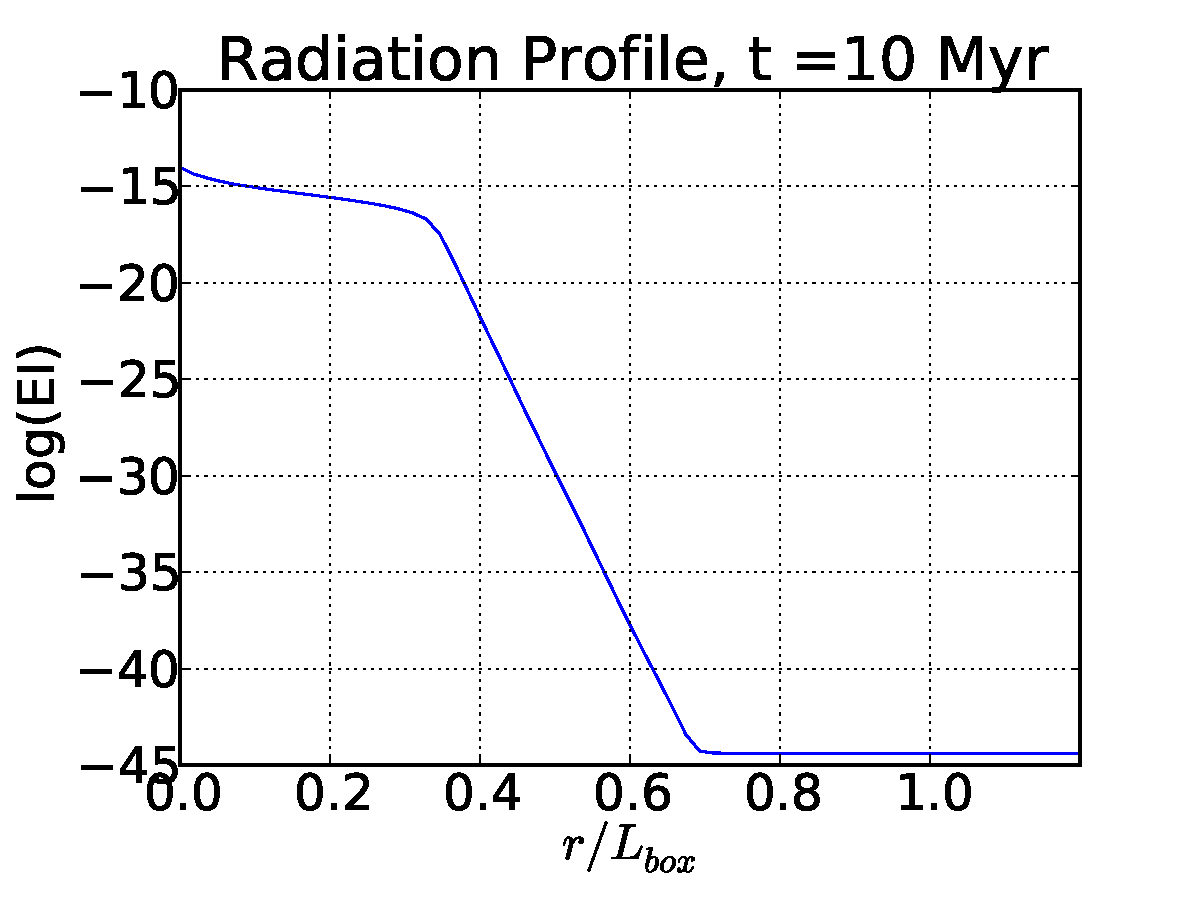
\includegraphics[scale=0.3, trim=1.0cm 0.5cm 1.0cm 0.5cm]{i1-Eprofiles_10Myr.eps}
  %% 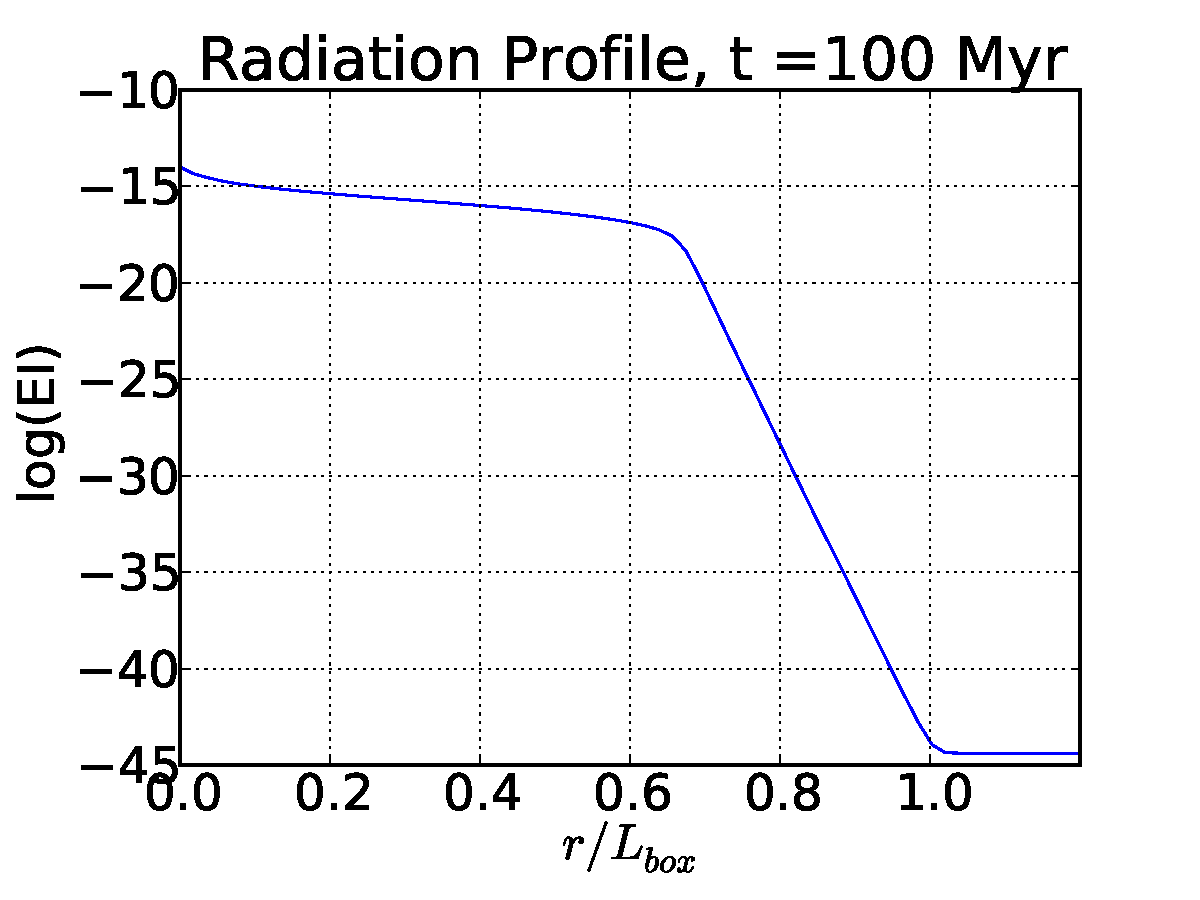
\includegraphics[scale=0.3, trim=1.0cm 0.5cm 1.0cm 0.5cm]{i1-Eprofiles_100Myr.eps}
  %% 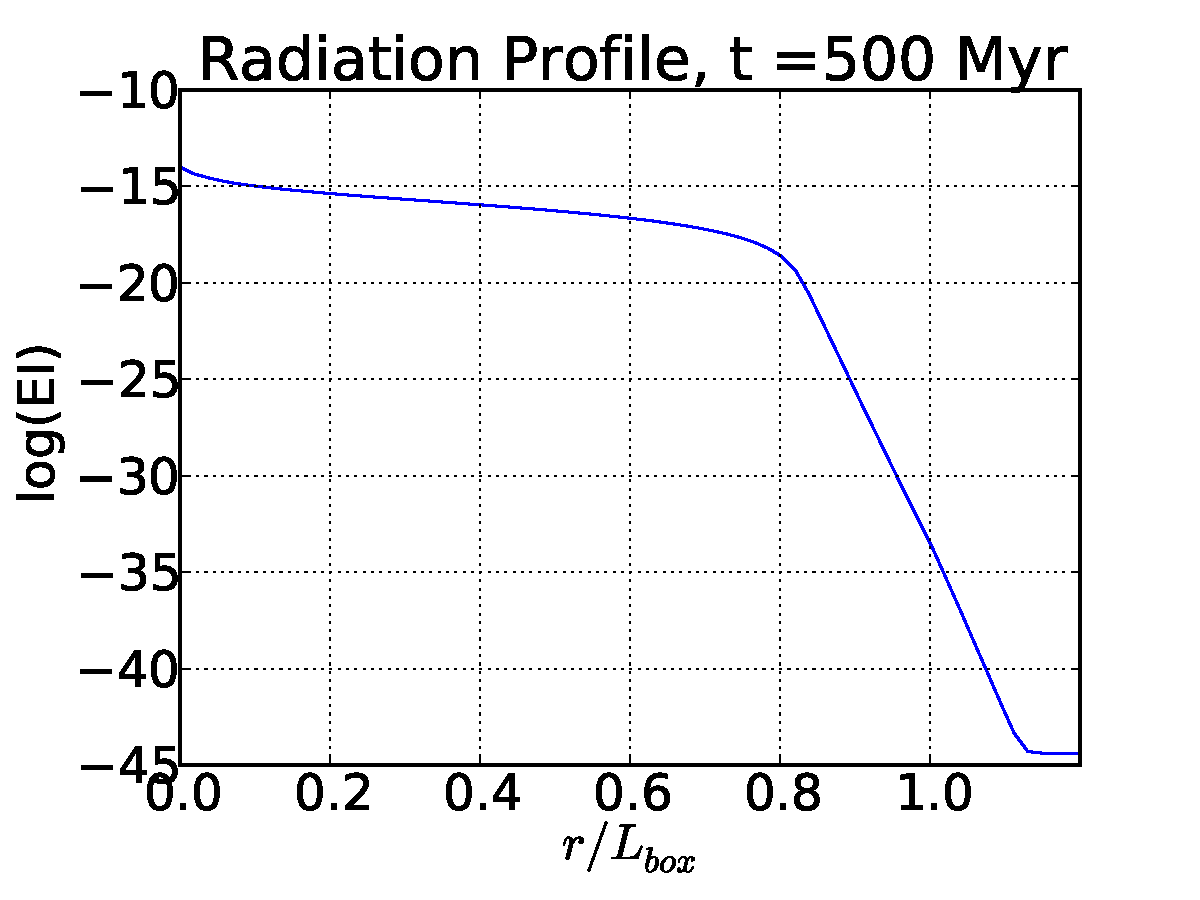
\includegraphics[scale=0.3, trim=1.0cm 0.5cm 1.0cm 0.5cm]{i1-Eprofiles_500Myr.eps}
  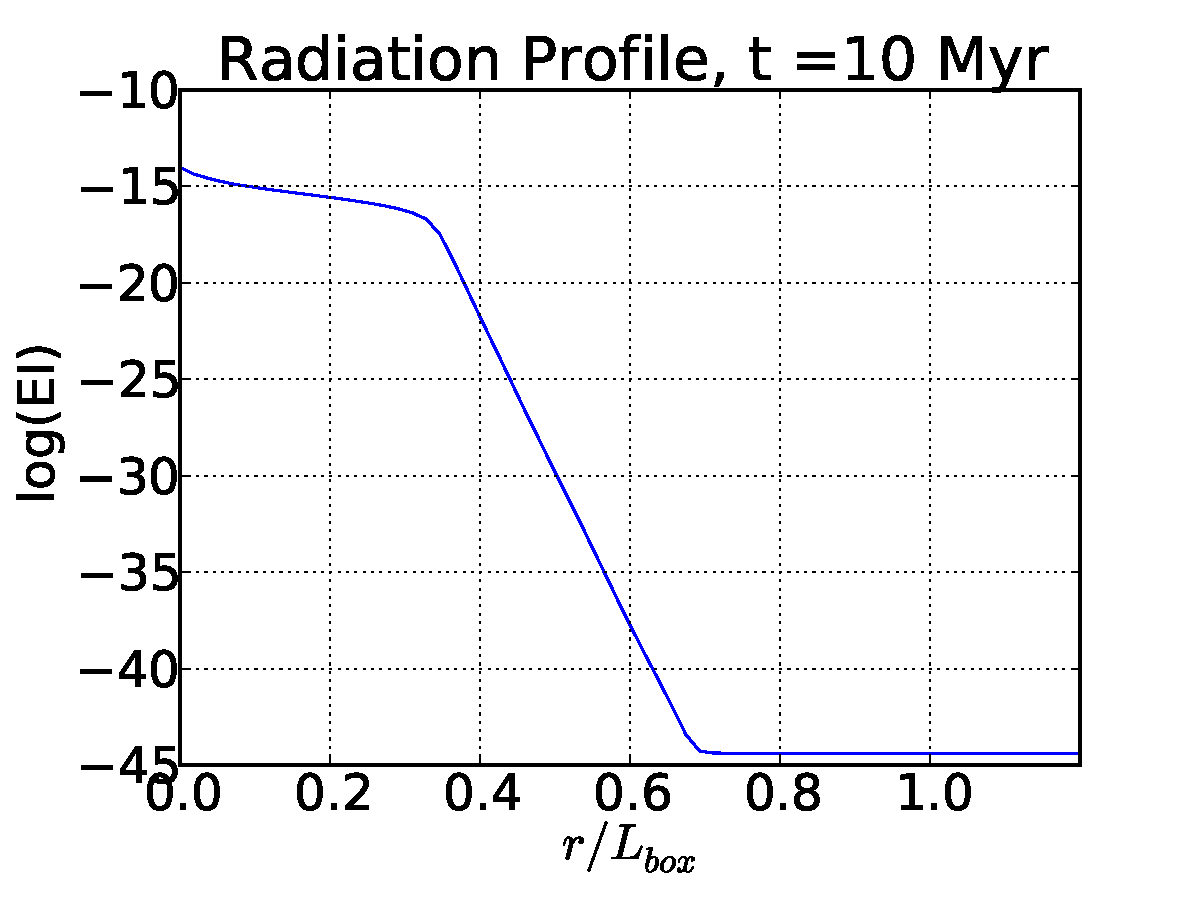
\includegraphics[scale=0.3, trim=1.0cm 1.0cm 1.0cm 0.5cm]{i1-Eprofiles_10Myr.pdf}
  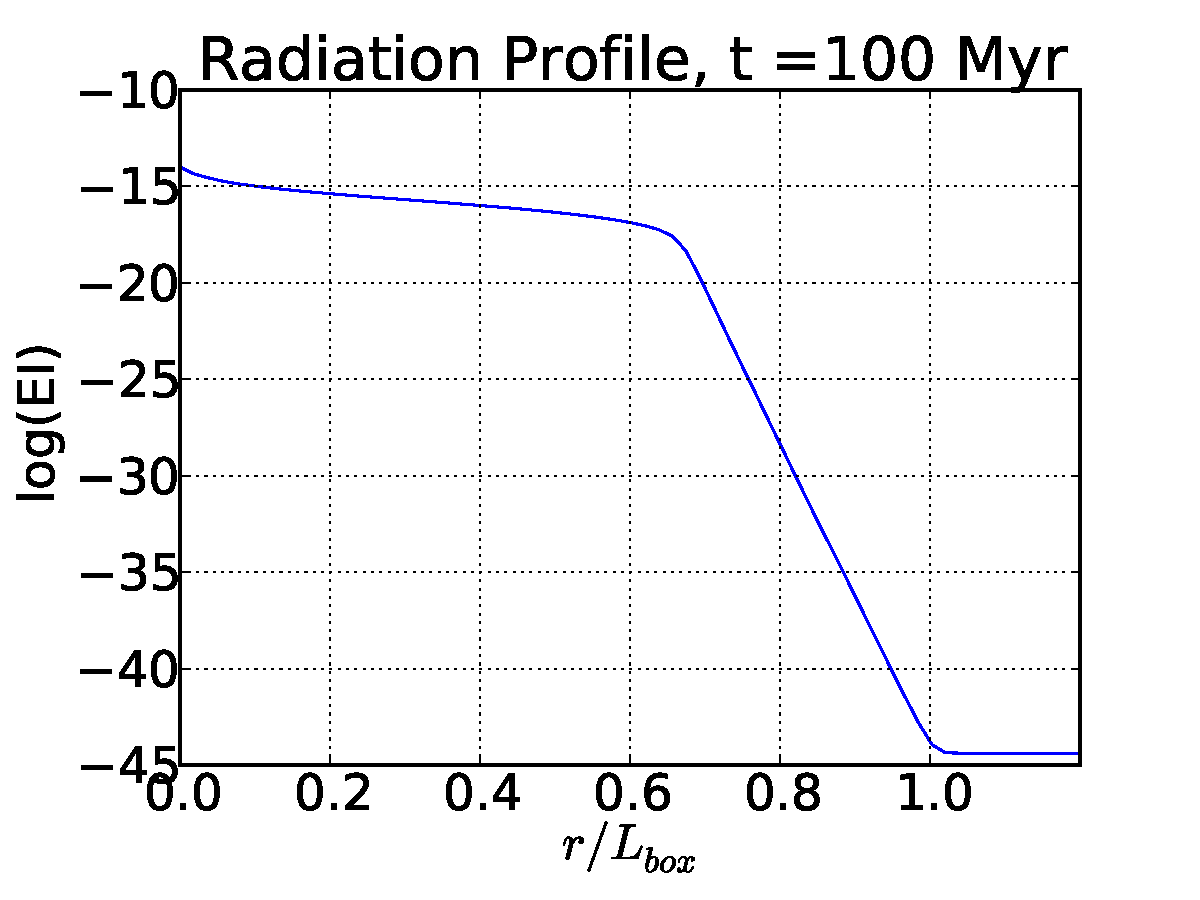
\includegraphics[scale=0.3, trim=1.0cm 1.0cm 1.0cm 0.5cm]{i1-Eprofiles_100Myr.pdf}
  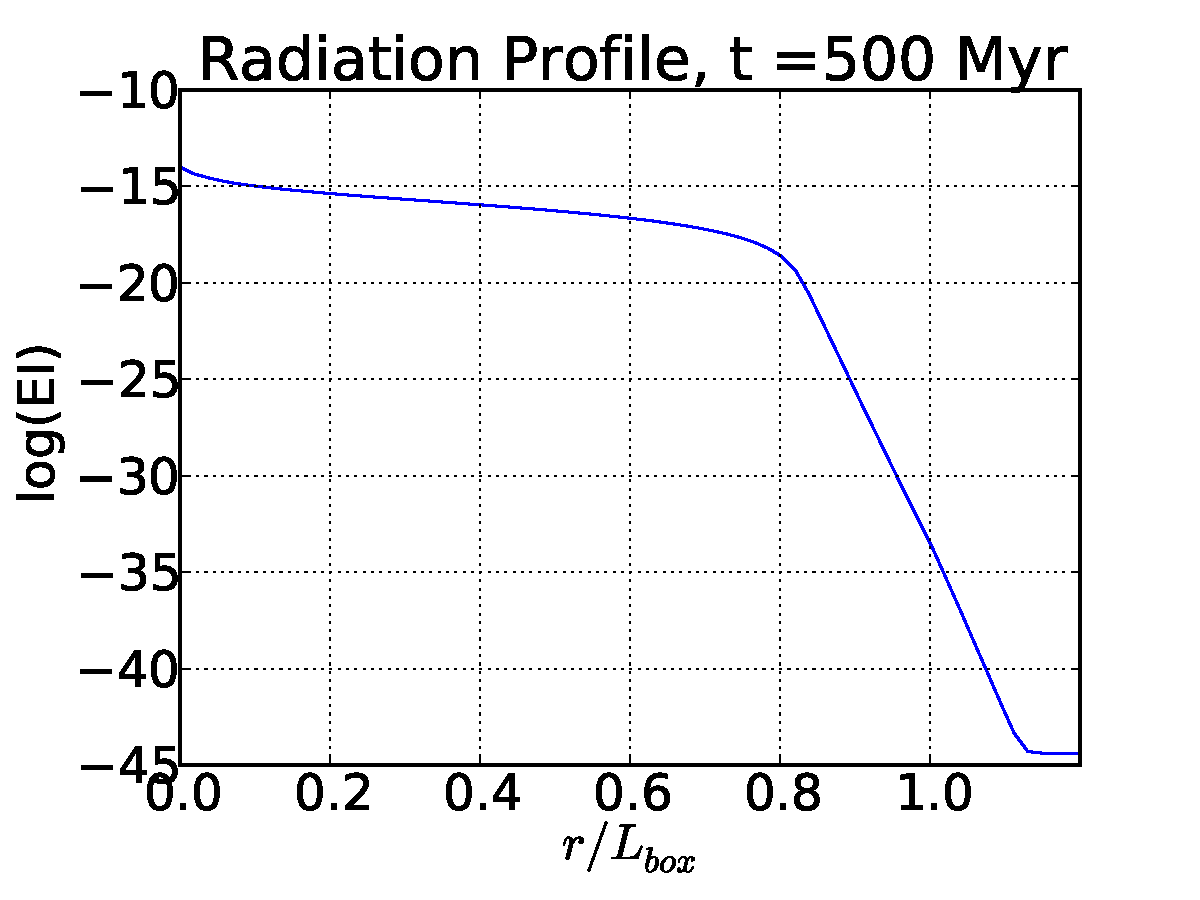
\includegraphics[scale=0.3, trim=1.0cm 1.0cm 1.0cm 0.5cm]{i1-Eprofiles_500Myr.pdf}
  \hfill}
\centerline{\hfill
  %% 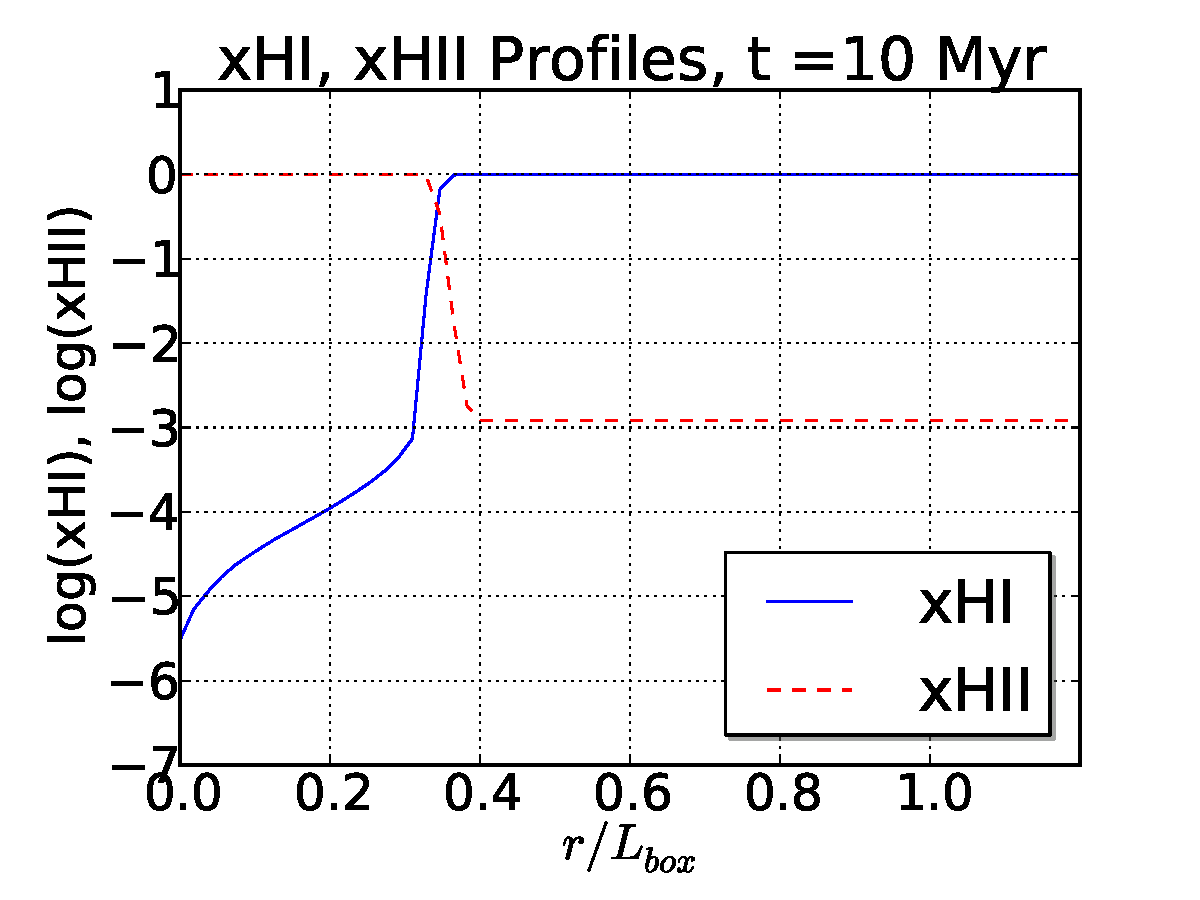
\includegraphics[scale=0.3, trim=1.0cm 0.5cm 1.0cm 0.5cm]{i1-profiles_10Myr.eps}
  %% 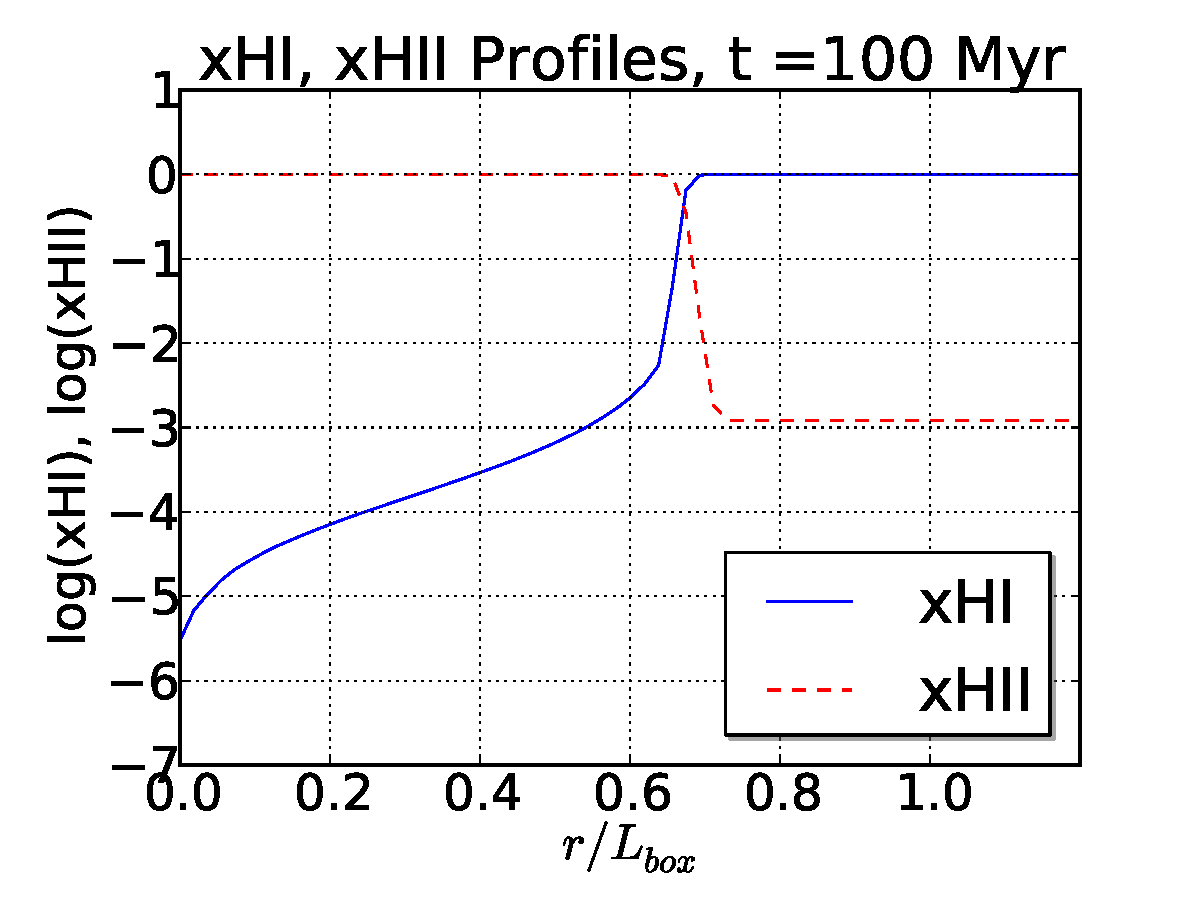
\includegraphics[scale=0.3, trim=1.0cm 0.5cm 1.0cm 0.5cm]{i1-profiles_100Myr.eps}
  %% 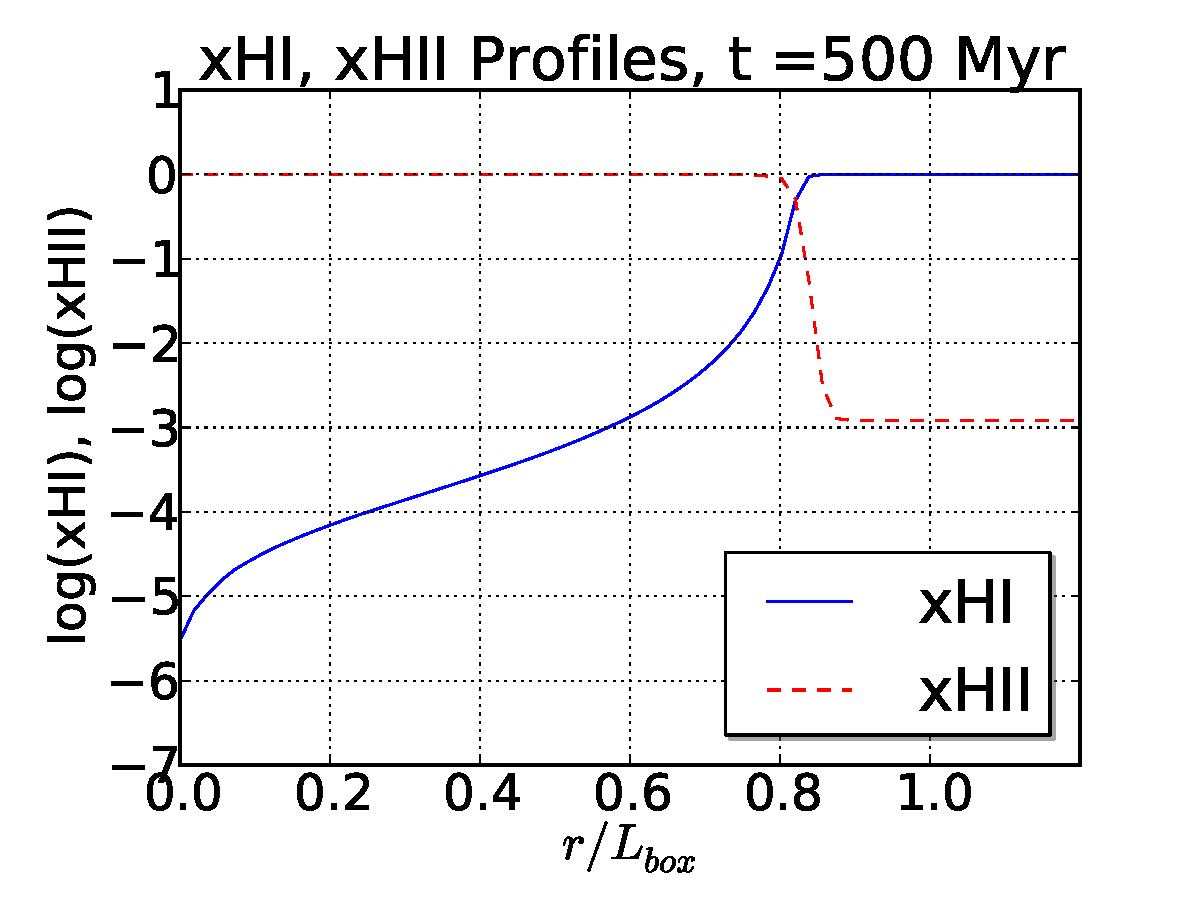
\includegraphics[scale=0.3, trim=1.0cm 0.5cm 1.0cm 0.5cm]{i1-profiles_500Myr.eps}
  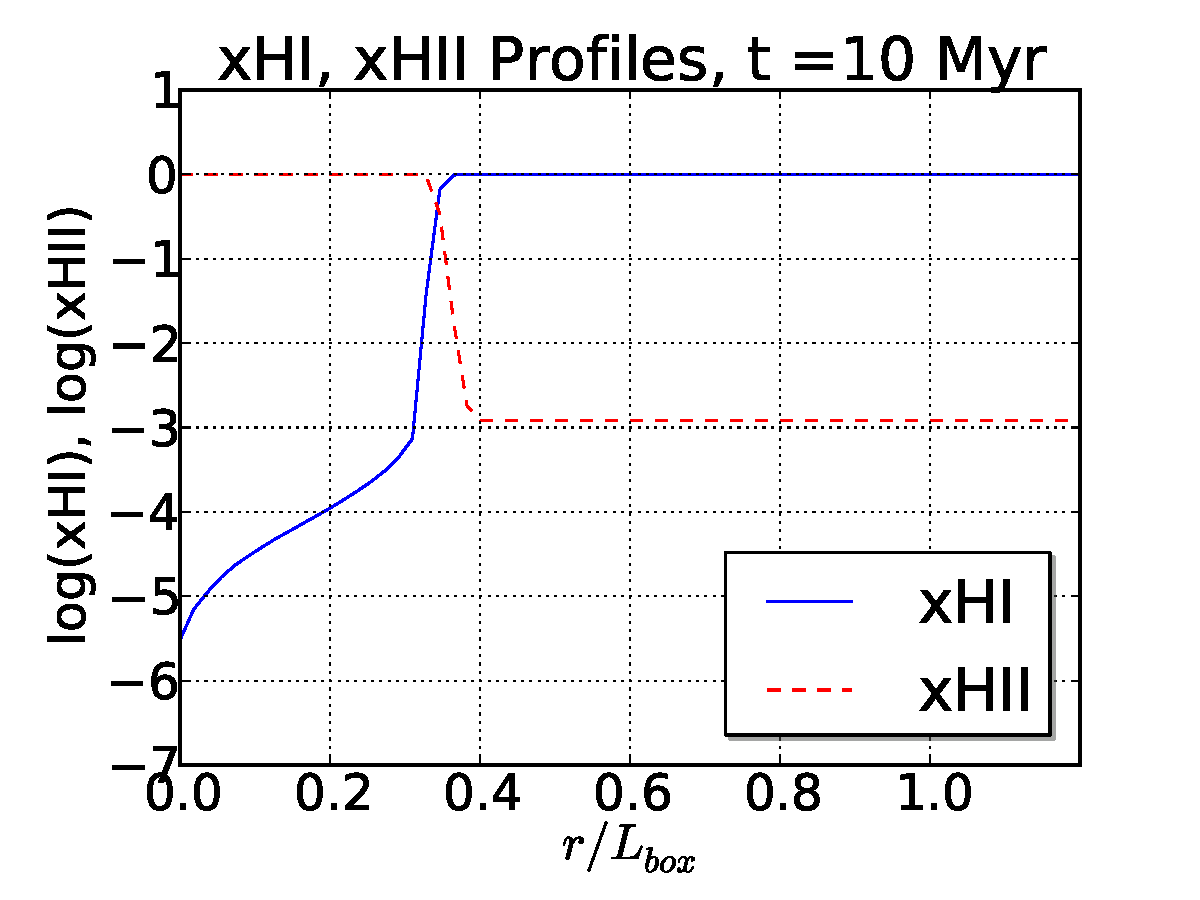
\includegraphics[scale=0.3, trim=1.0cm 0.5cm 1.0cm 0.5cm]{i1-profiles_10Myr.pdf}
  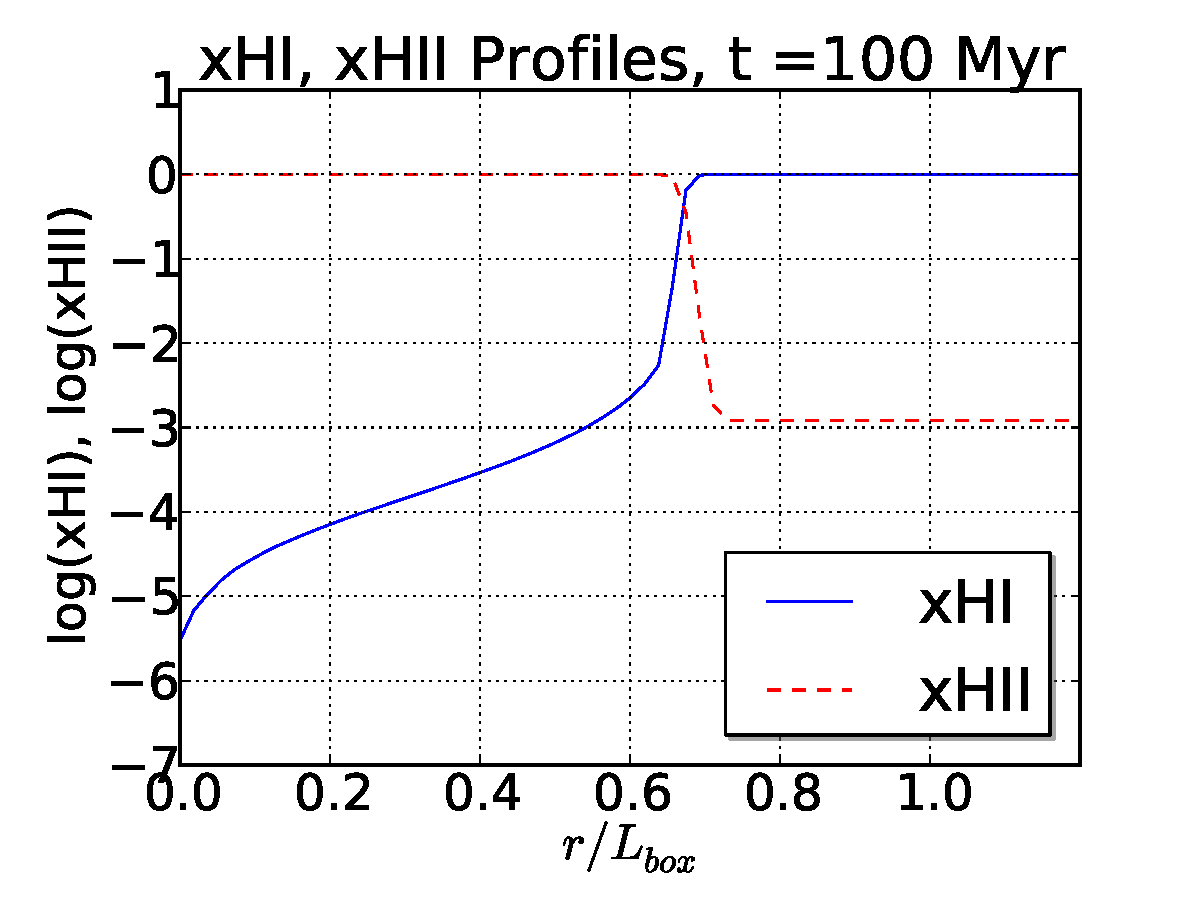
\includegraphics[scale=0.3, trim=1.0cm 0.5cm 1.0cm 0.5cm]{i1-profiles_100Myr.pdf}
  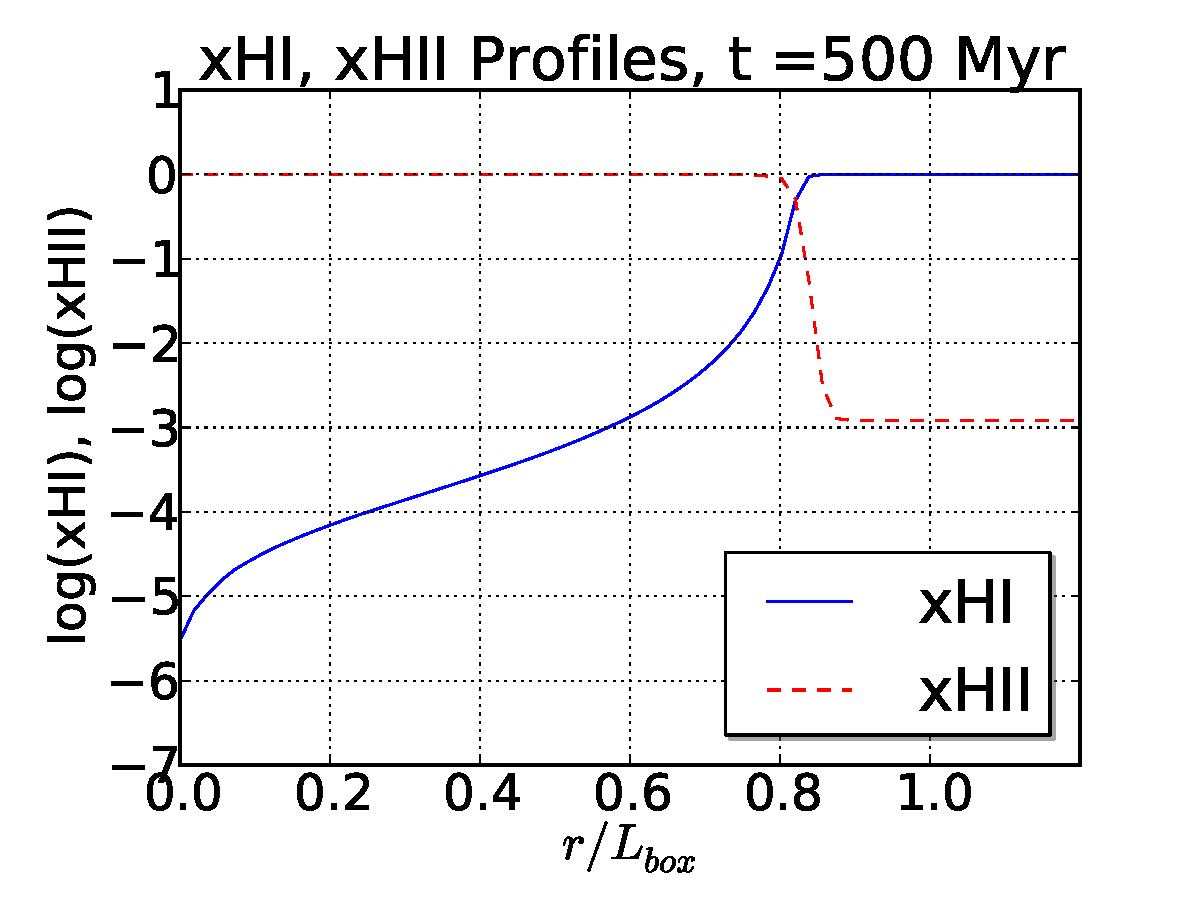
\includegraphics[scale=0.3, trim=1.0cm 0.5cm 1.0cm 0.5cm]{i1-profiles_500Myr.pdf}
  \hfill}
  \caption{Spherically-averaged radial profiles of radiation energy
    density and ionization fractions for the isothermal ionization
    test in section \ref{subsec:test1} using a $128^3$ mesh and
    time step tolerance $\tau_{tol} =10^{-4}$.  Plots are shown at 10, 100
    and 500 Myr (left to right), with the radiation energy density on
    the top row and ionization fractions on the bottom row.}
  \label{fig:i1_results}
\end{figure}
Plots of the computed and analytical I front position and resulting
error for this run are provided in Figure \ref{fig:i1_radius}.
\begin{figure}[t]
\centerline{\hfill
  %% 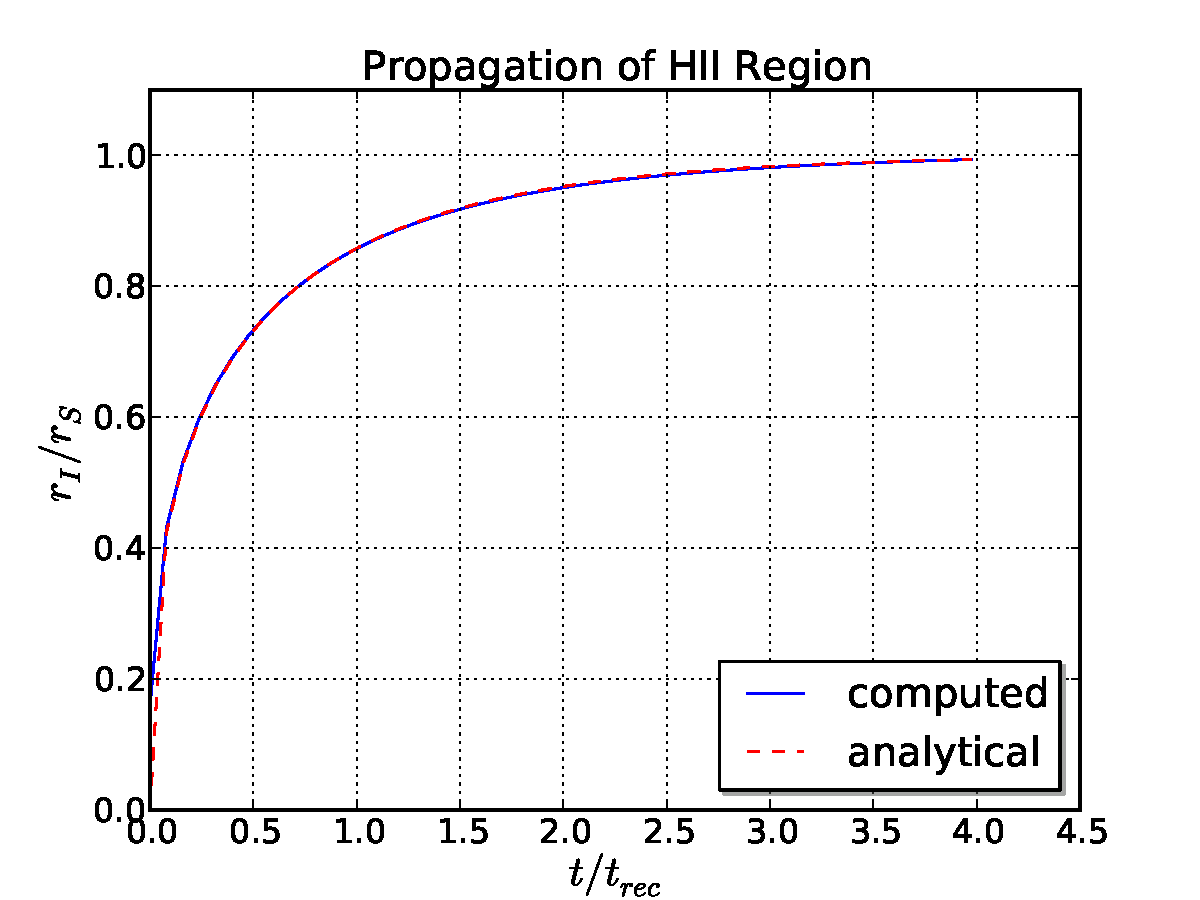
\includegraphics[scale=0.45, trim=1.0cm 0.5cm 1.0cm 0.5cm]{i1-rad_vs_time.eps}
  %% 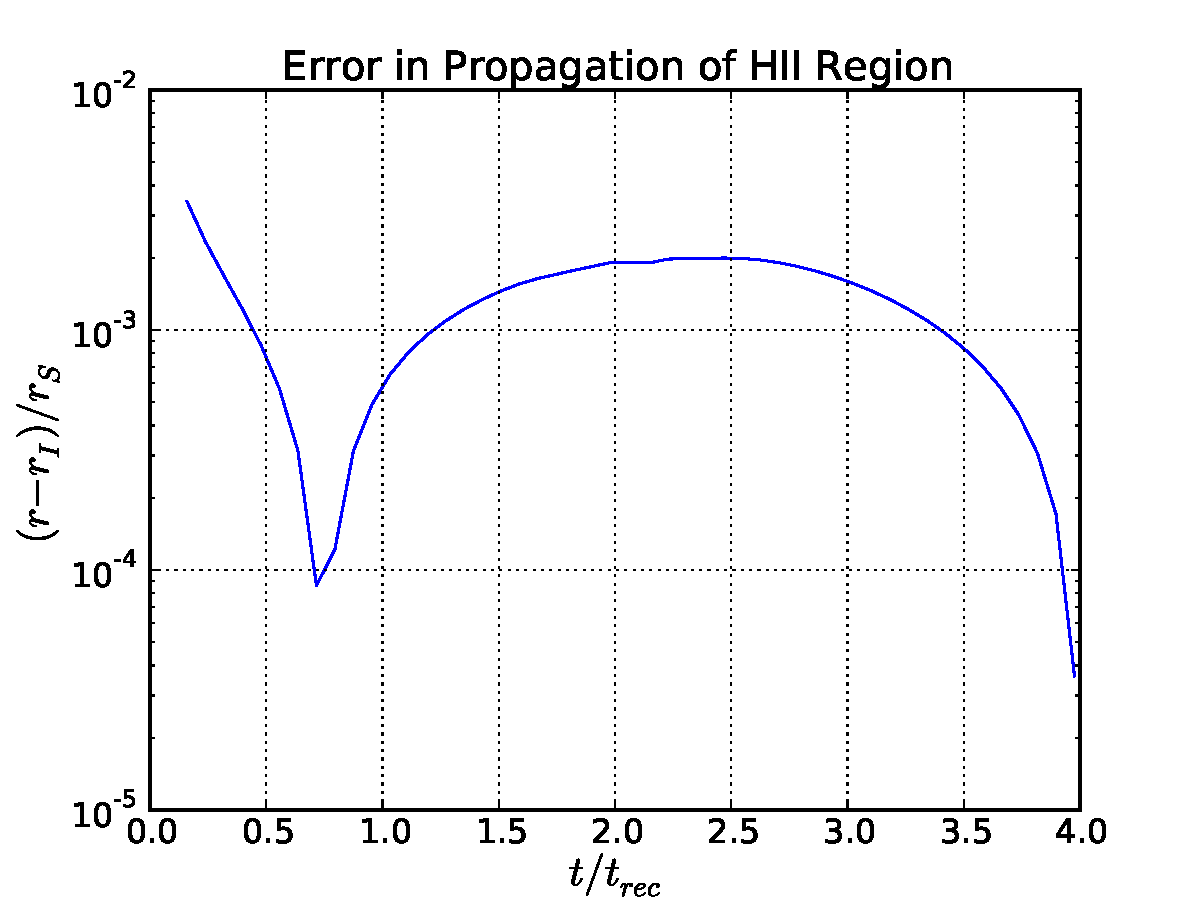
\includegraphics[scale=0.45, trim=1.0cm 0.5cm 1.0cm 0.5cm]{i1-rad_error_vs_time.eps}
  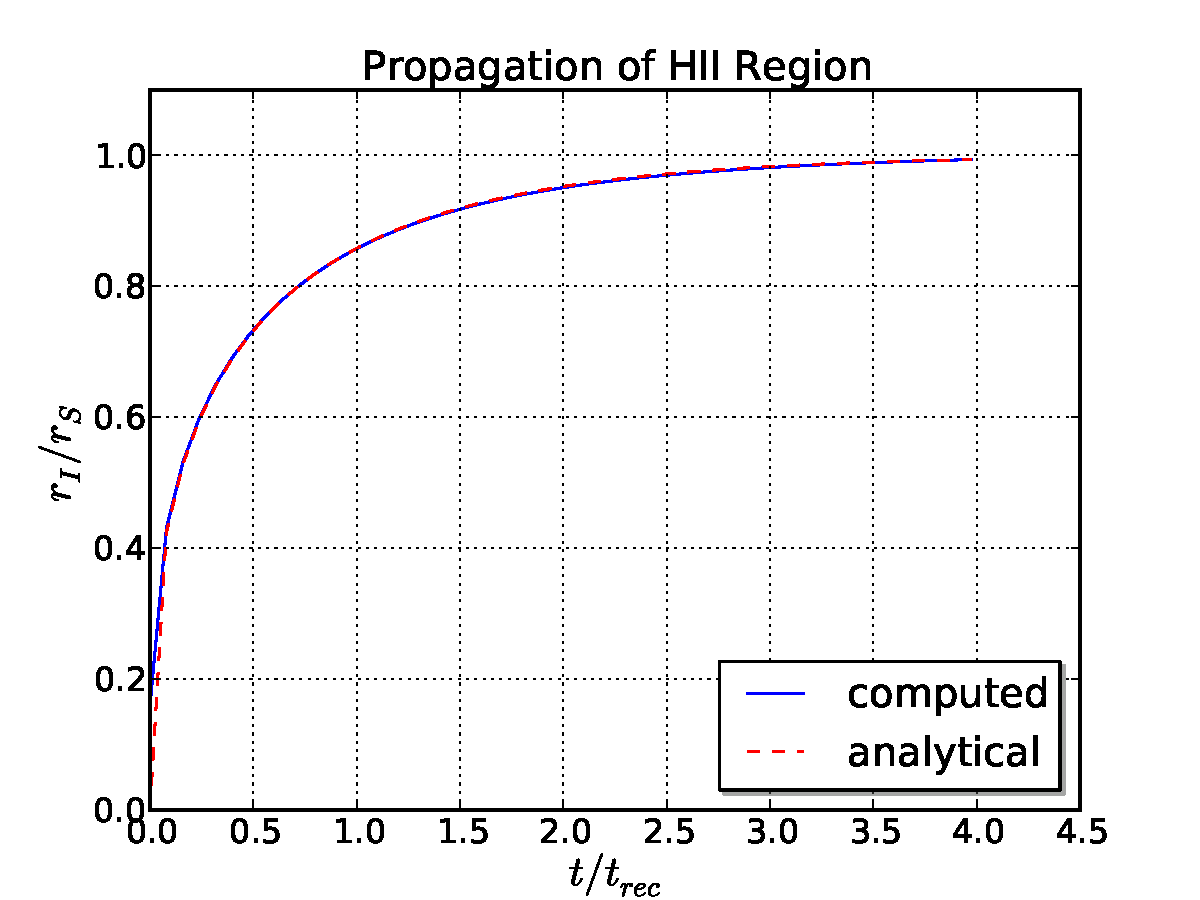
\includegraphics[scale=0.45, trim=1.0cm 0.5cm 1.0cm 0.5cm]{i1-rad_vs_time.pdf}
  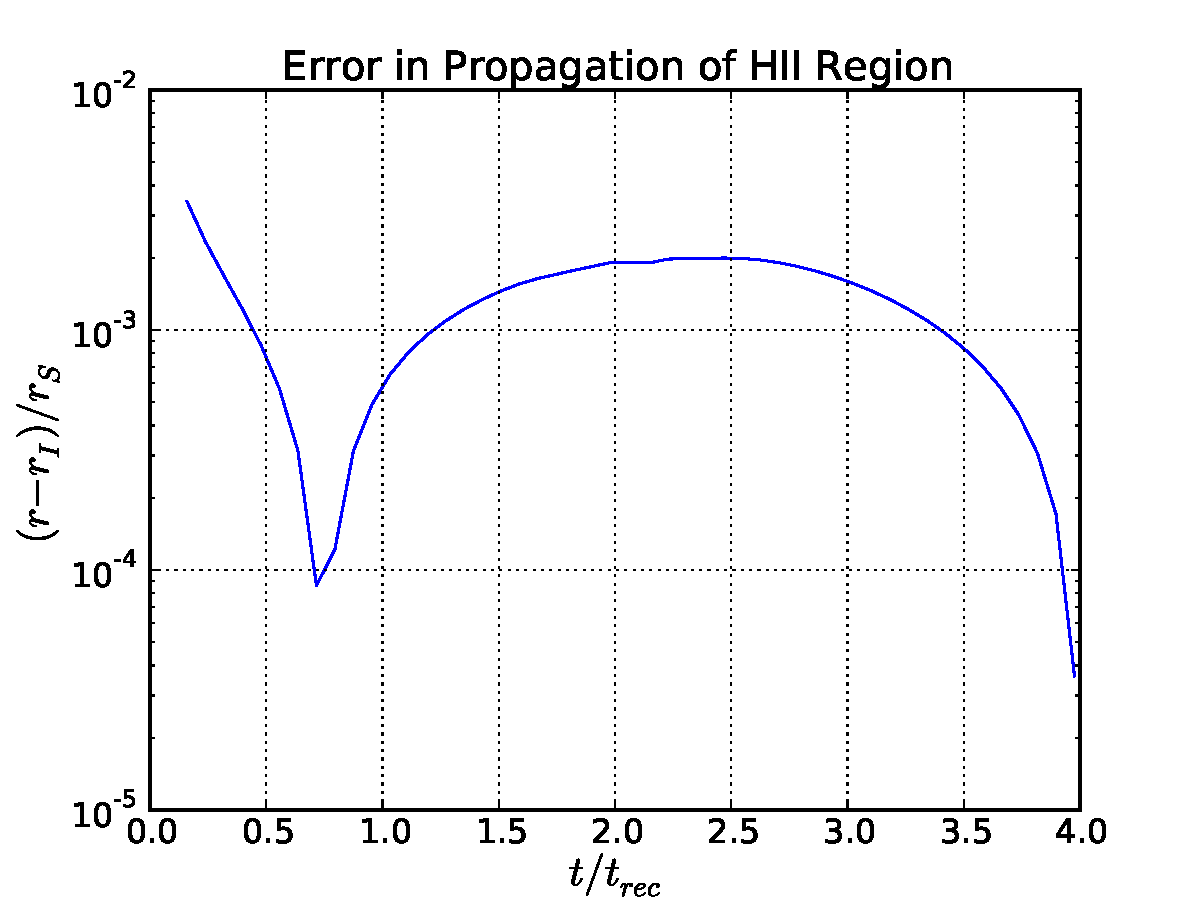
\includegraphics[scale=0.45, trim=1.0cm 0.5cm 1.0cm 0.5cm]{i1-rad_error_vs_time.pdf}
  \hfill}
  \caption{Comparison between computed and analytical I front position
    for the isothermal ionization test in section \ref{subsec:test1}
    using a $128^3$ mesh and time step tolerance $\tau_{tol}
    =10^{-4}$. Solution on left, error on right.} 
  \label{fig:i1_radius}
\end{figure}
To further investigate the accuracy of our new splitting approach
between the radiation and chemistry solvers, we then performed these
same tests at a variety of mesh sizes and time step tolerances 
$\tau_{tol}$.  For mesh sizes of $16^3$, $32^3$ and $64^3$, and for
tolerances $10^{-2}$, $10^{-3}$, $10^{-4}$ and $10^{-5}$, we
compute the error in the I front position as
\begin{equation}
\label{eq:i1_error}
   error \ = \ \left\| \frac{r_{computed} - r_{true}}{r_s} \right\|_{RMS}
   \ = \ \left(\frac{1}{N_t} \sum_{i=1}^{N_t} \left(\frac{r_{computed,i} -
       r_{true,i}}{r_s}\right)^2 \right)^{1/2}.
\end{equation}
In Figure \ref{fig:i1_stats}, we plot the solution error as a function
of the average time step size, as well as the total runtime as a
function of the average time step size.  
\begin{figure}[t]
\centerline{\hfill
  %% 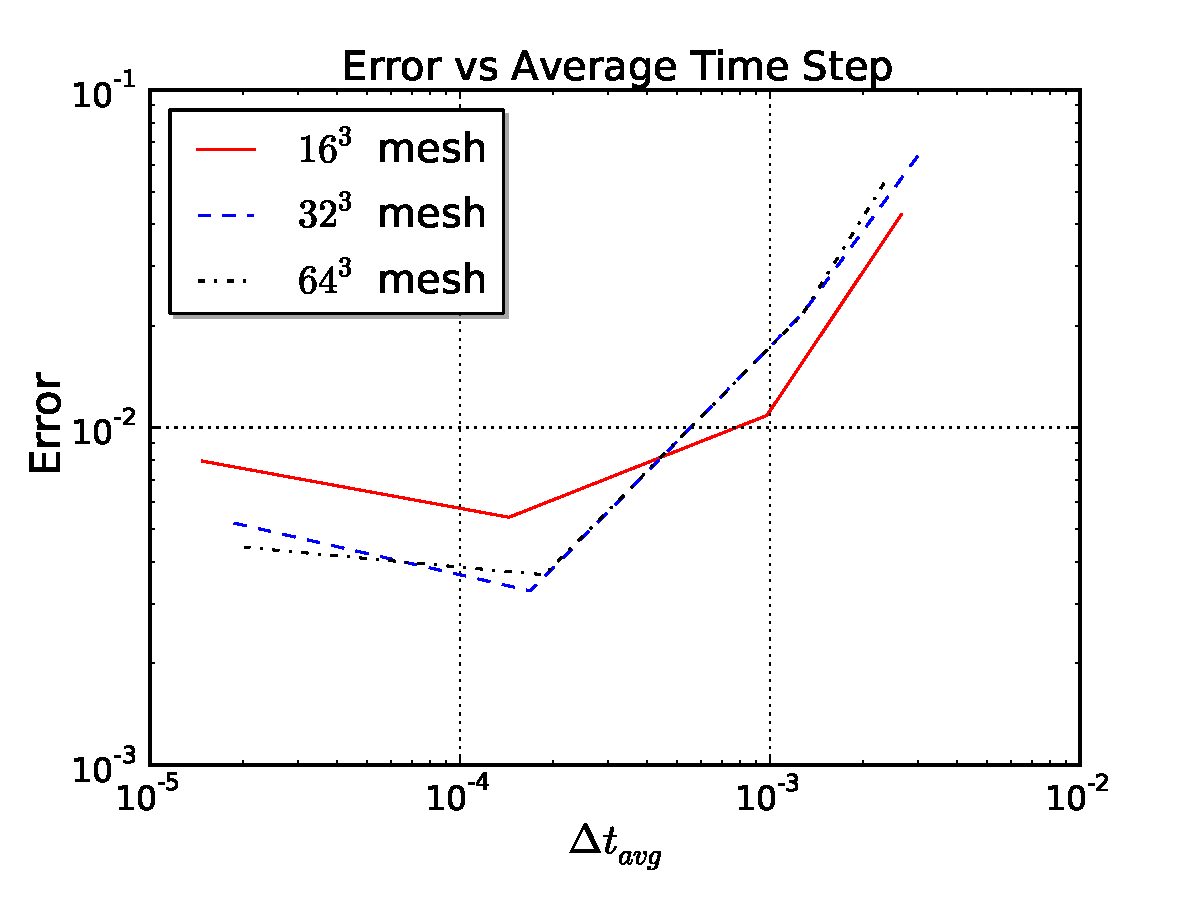
\includegraphics[scale=0.45, trim=1.0cm 0.5cm 1.0cm 0.5cm]{i1-error_enzo.eps}
  %% 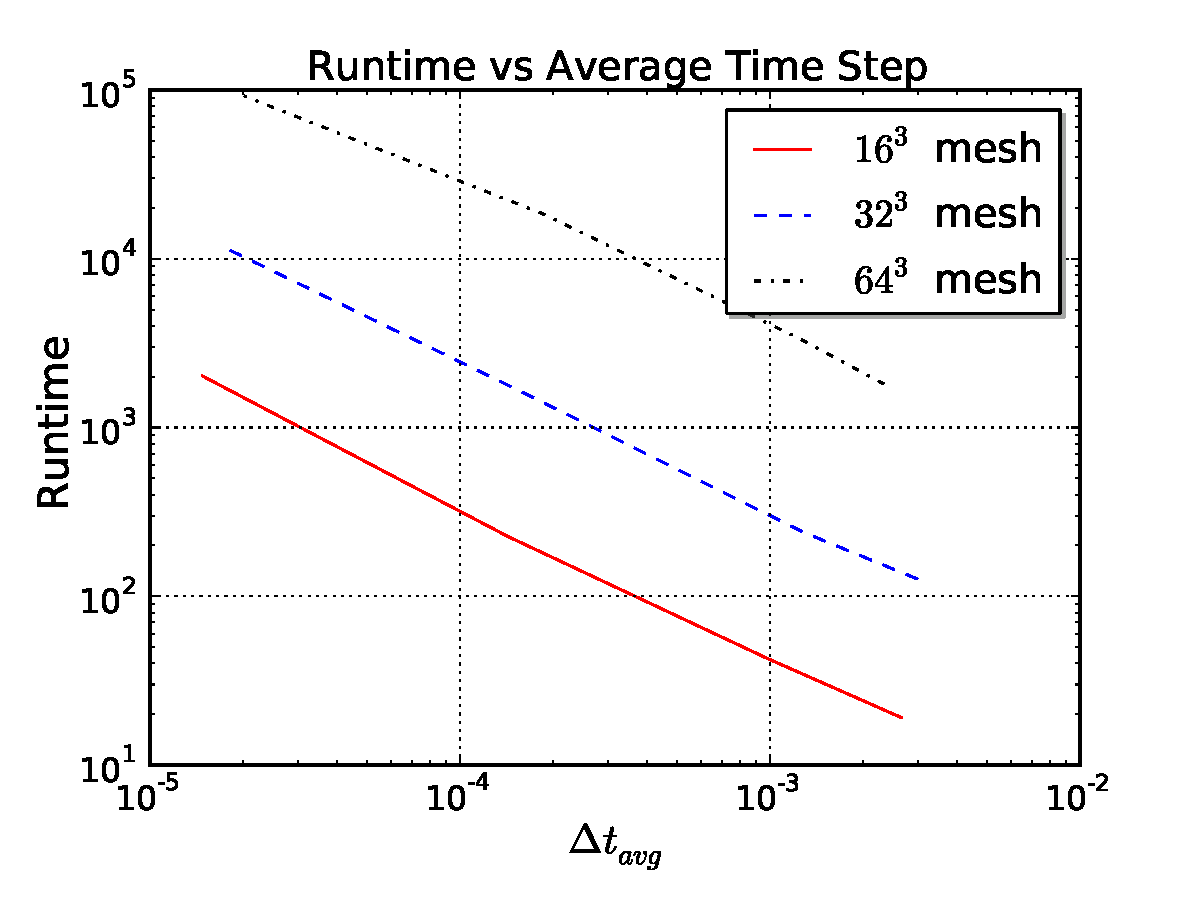
\includegraphics[scale=0.45, trim=1.0cm 0.5cm 1.0cm 0.5cm]{i1-runtime_enzo.eps}
  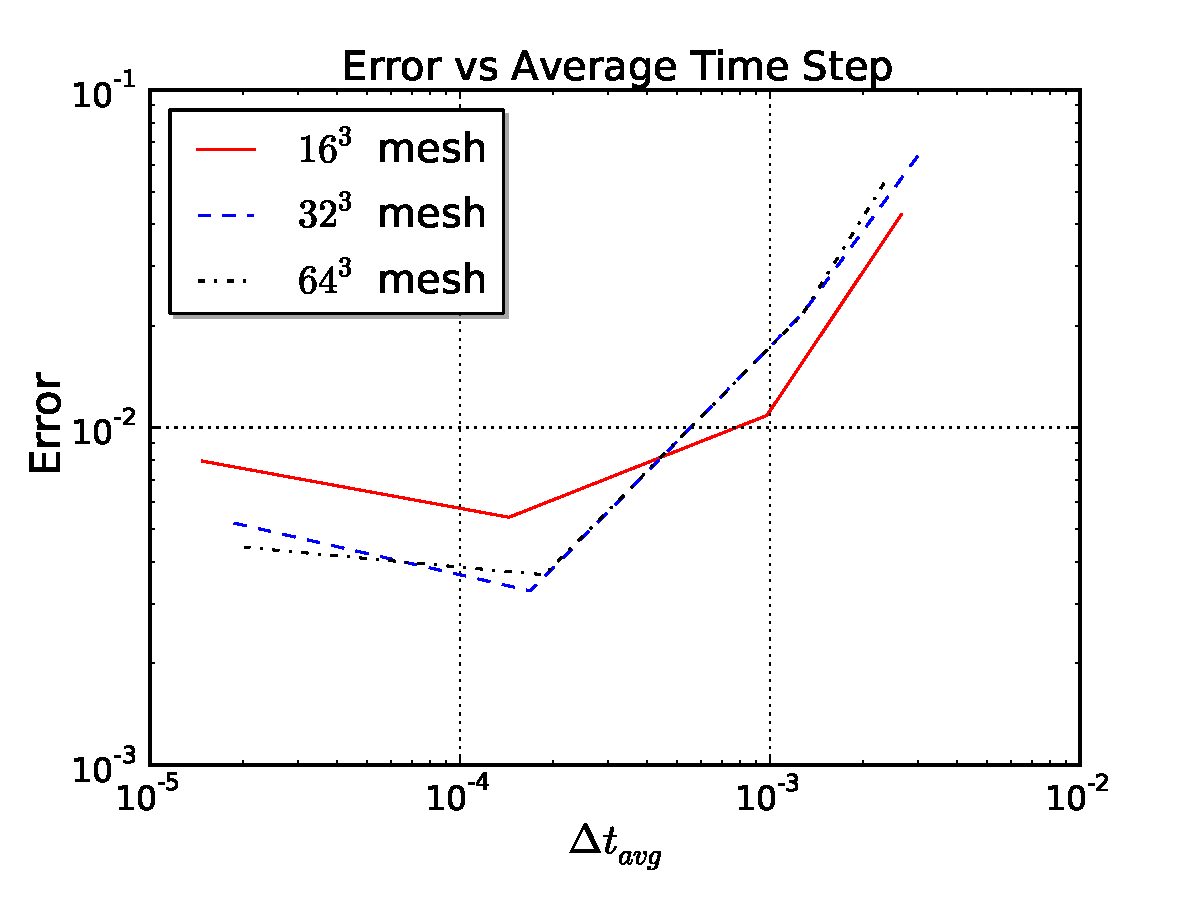
\includegraphics[scale=0.45, trim=1.0cm 0.0cm 1.0cm 0.5cm]{i1-error_enzo.pdf}
  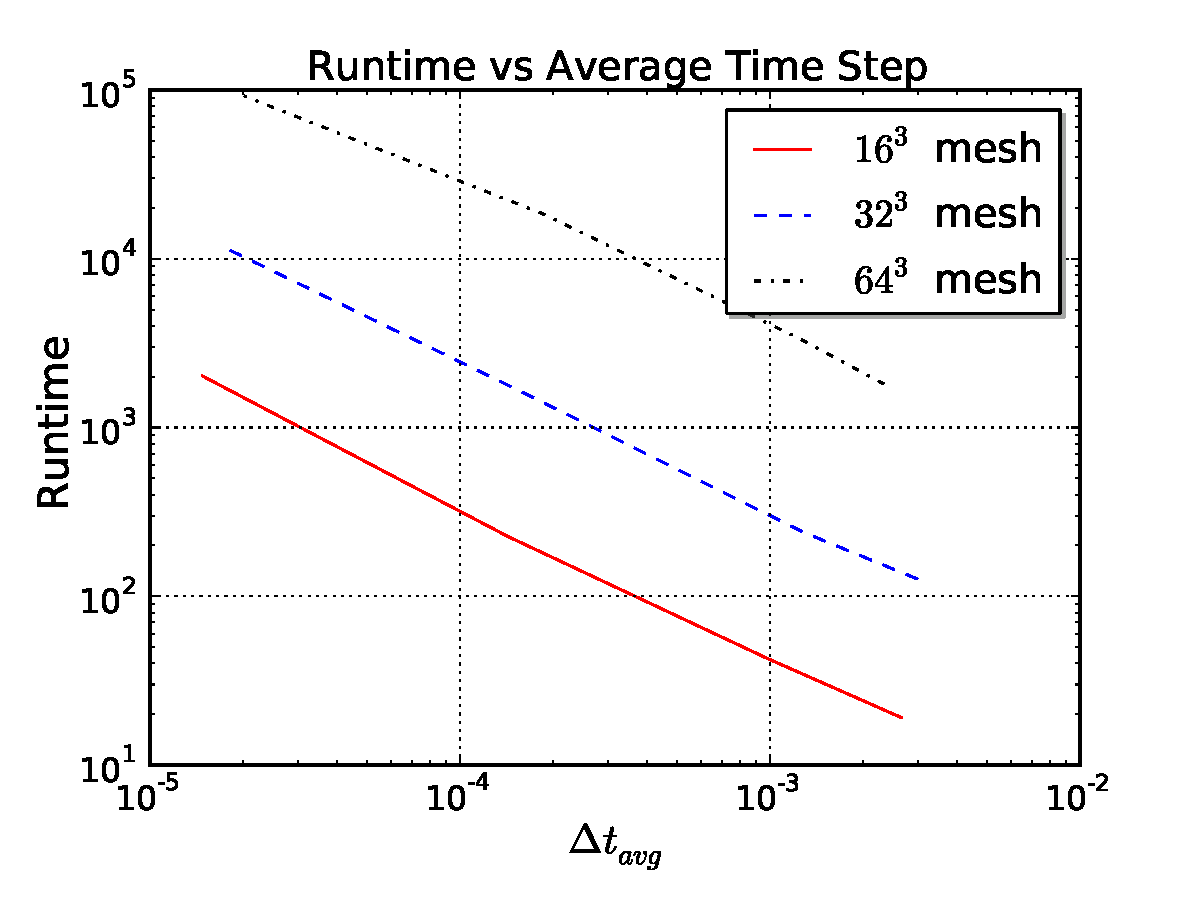
\includegraphics[scale=0.45, trim=1.0cm 0.0cm 1.0cm 0.5cm]{i1-runtime_enzo.pdf}
  \hfill}
  \caption{We ran tests using mesh sizes of
    $16^3$, $32^3$ and $64^4$, and time step tolerances of
    $10^{-2}$, $10^{-3}$, $10^{-4}$ and $10^{-5}$, and plot the I
    front position error \eqref{eq:i1_error} as a function of the
    average time step size.  As expected, the runtime scales linearly
    with the inverse $\Delta t_{avg}$, and the error scales linearly
    with $\Delta t_{avg}$, at least until other sources of error
    dominate the calculation.}
  \label{fig:i1_stats}
\end{figure}
As can be seen in these plots, as the tolerance decreases, the
temporal solution accuracy increases linearly until we reach a minimum
accuracy that results from other components in Enzo (spatial
discretization accuracy, accuracy within Enzo's chemistry solver,
etc.).  Moreover, it is evident that as we decrease the time step
tolerances, the required runtime increases linearly.  These results
imply that there is a ``sweet spot'' in our approach, wherein a
tolerance of $\tau_{tol}=10^{-4}$ achieves the solution with optimal
accuracy before we begin to waste additional effort without achieving
accuracy improvements.  {\bf While this specific value is likely
problem-dependent, we use it as a starting point in subsequent
simulations. }

Finally, in Figure \ref{fig:i1_contours} we plot a slice of the
computed HII region through the center of the domain, perpendicular to
the $z$-direction (other directions are equivalent), to show the
convergence of the ionized region to a sphere at varying spatial
resolutions.
\begin{figure}[t]
\centerline{\hfill
  %% 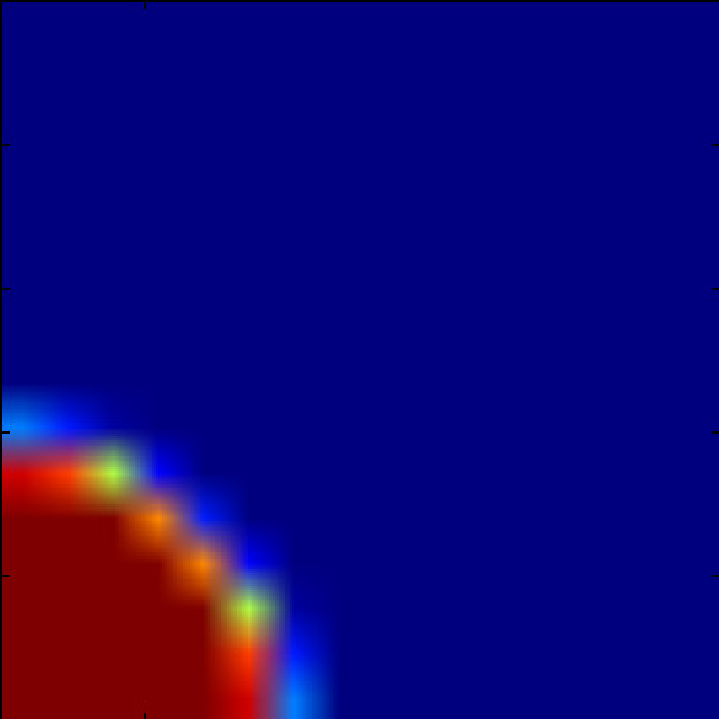
\includegraphics[scale=0.3]{i1-HIIcontour_10myr_nx16.eps}
  %% \hspace{0.1cm}
  %% 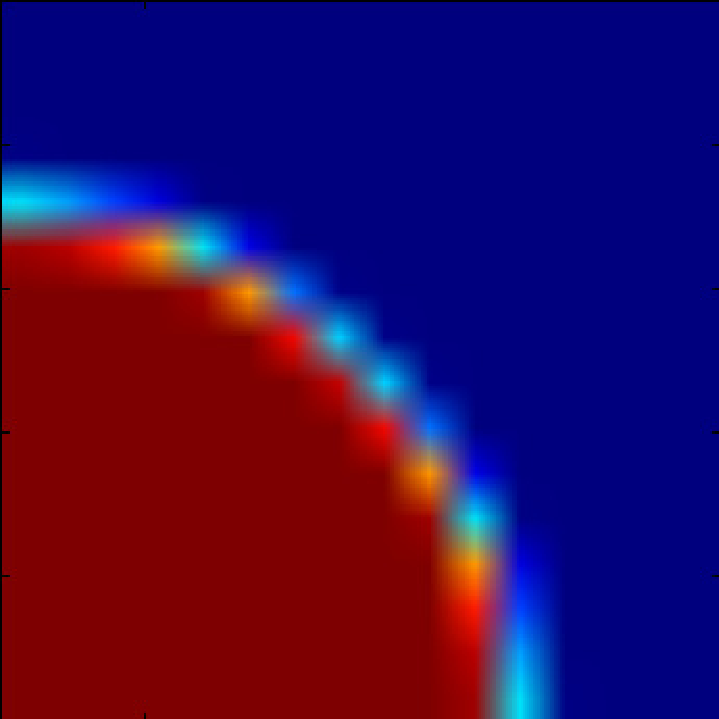
\includegraphics[scale=0.3]{i1-HIIcontour_100myr_nx16.eps}
  %% \hspace{0.1cm}
  %% 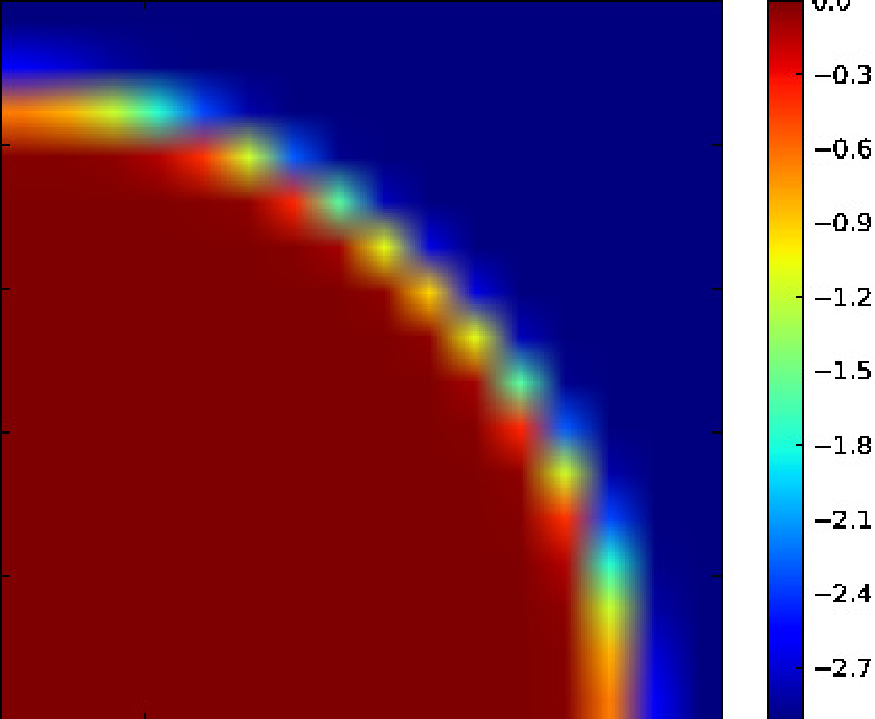
\includegraphics[scale=0.3]{i1-HIIcontour_500myr_nx16.eps}
  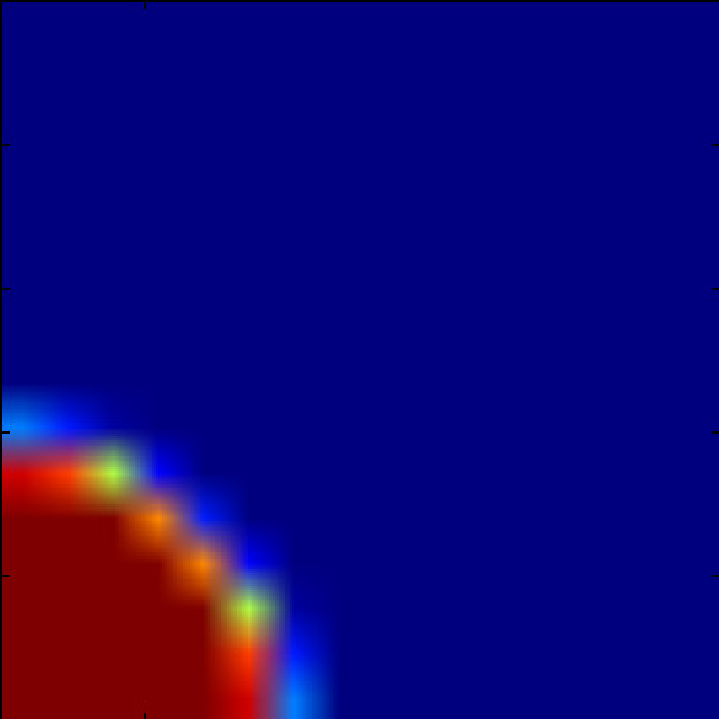
\includegraphics[scale=0.3]{i1-HIIcontour_10myr_nx16.pdf}
  \hspace{0.1cm}
  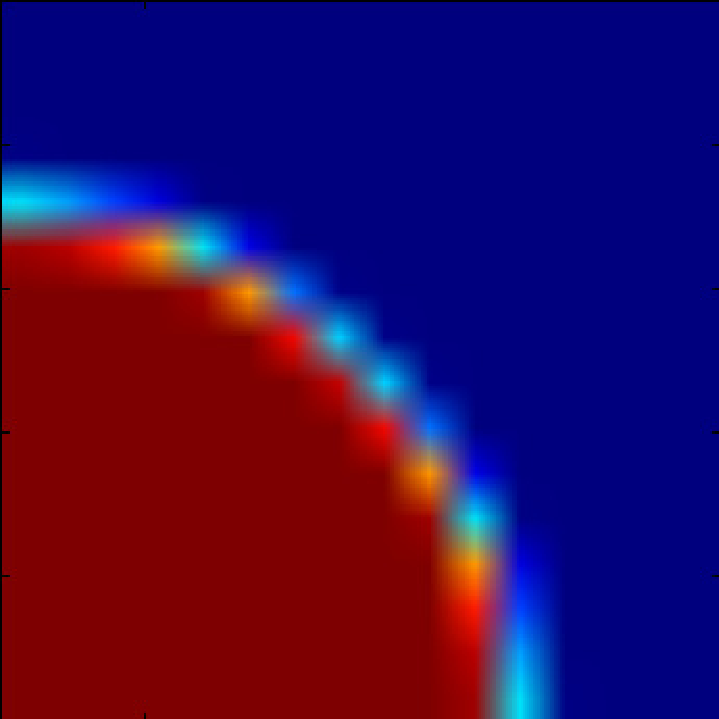
\includegraphics[scale=0.3]{i1-HIIcontour_100myr_nx16.pdf}
  \hspace{0.1cm}
  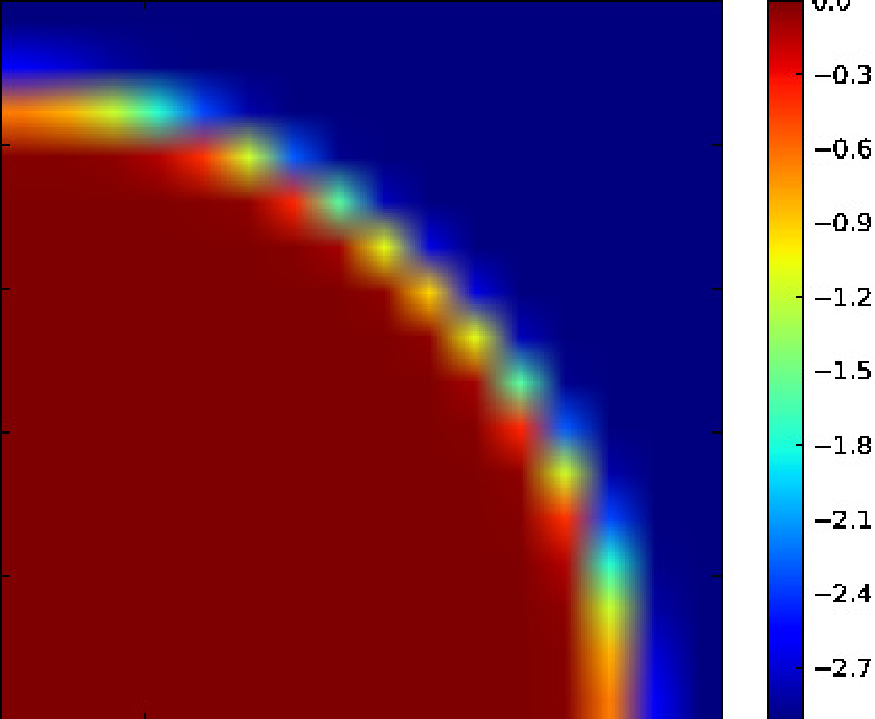
\includegraphics[scale=0.3]{i1-HIIcontour_500myr_nx16.pdf}
  \hfill}
\vspace{0.2cm}
\centerline{\hfill
  %% 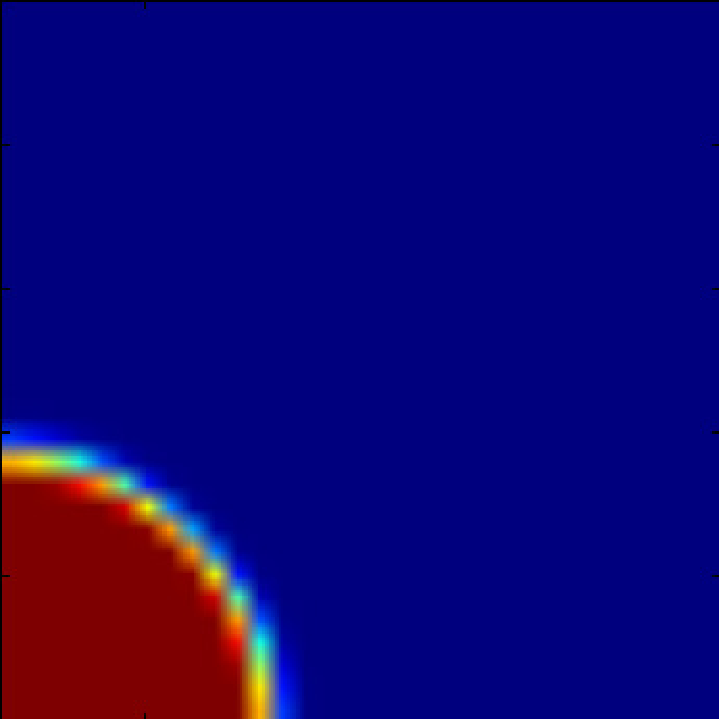
\includegraphics[scale=0.3]{i1-HIIcontour_10myr_nx32.eps}
  %% \hspace{0.1cm}
  %% 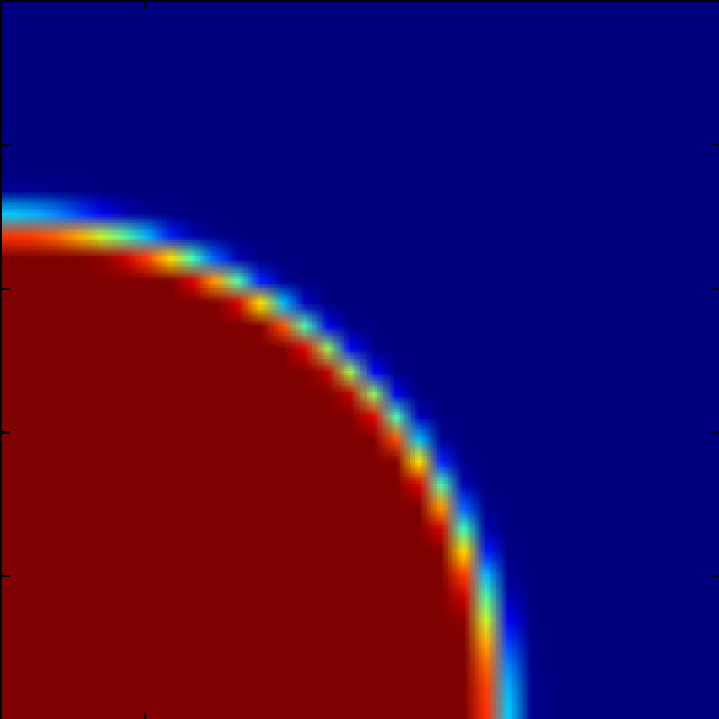
\includegraphics[scale=0.3]{i1-HIIcontour_100myr_nx32.eps}
  %% \hspace{0.1cm}
  %% 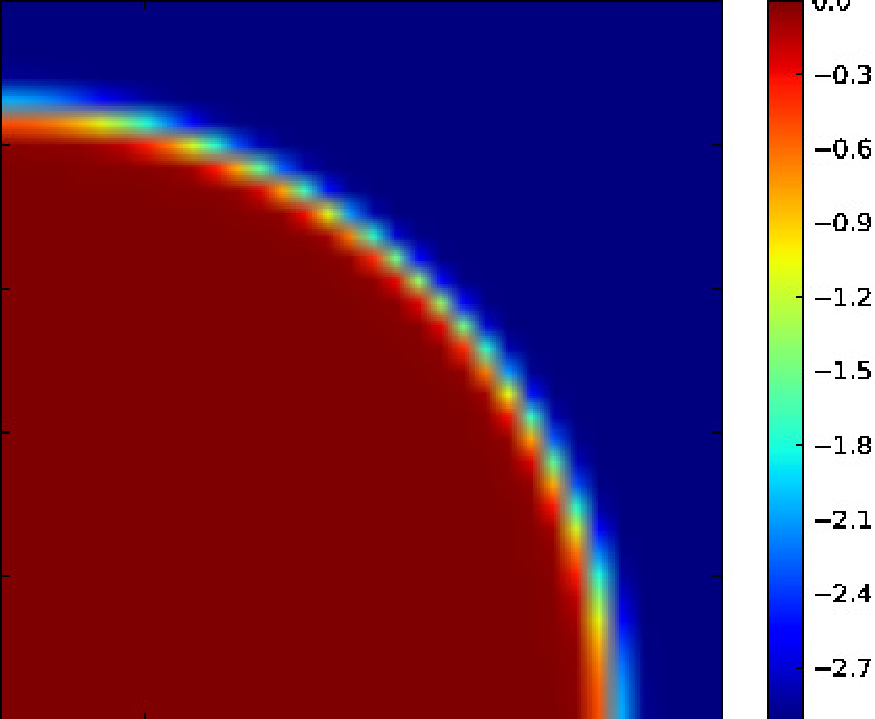
\includegraphics[scale=0.3]{i1-HIIcontour_500myr_nx32.eps}
  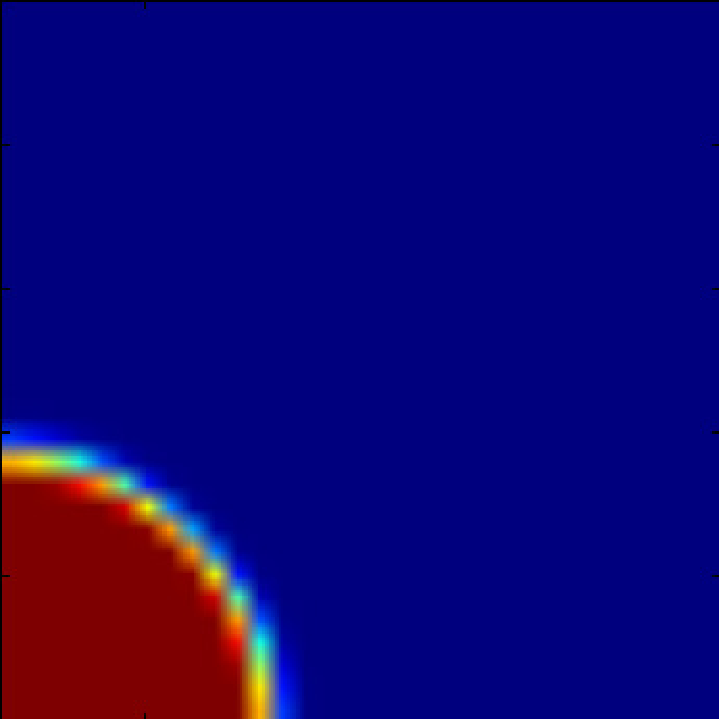
\includegraphics[scale=0.3]{i1-HIIcontour_10myr_nx32.pdf}
  \hspace{0.1cm}
  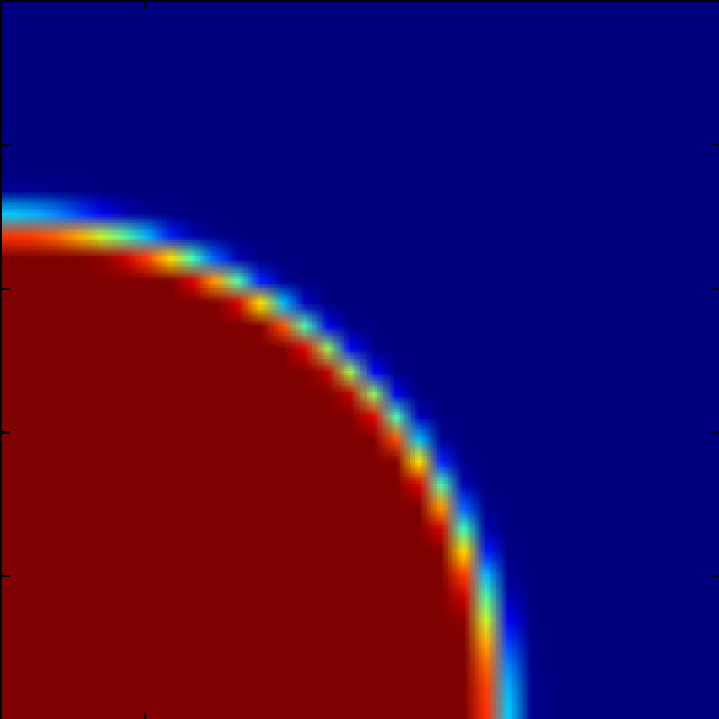
\includegraphics[scale=0.3]{i1-HIIcontour_100myr_nx32.pdf}
  \hspace{0.1cm}
  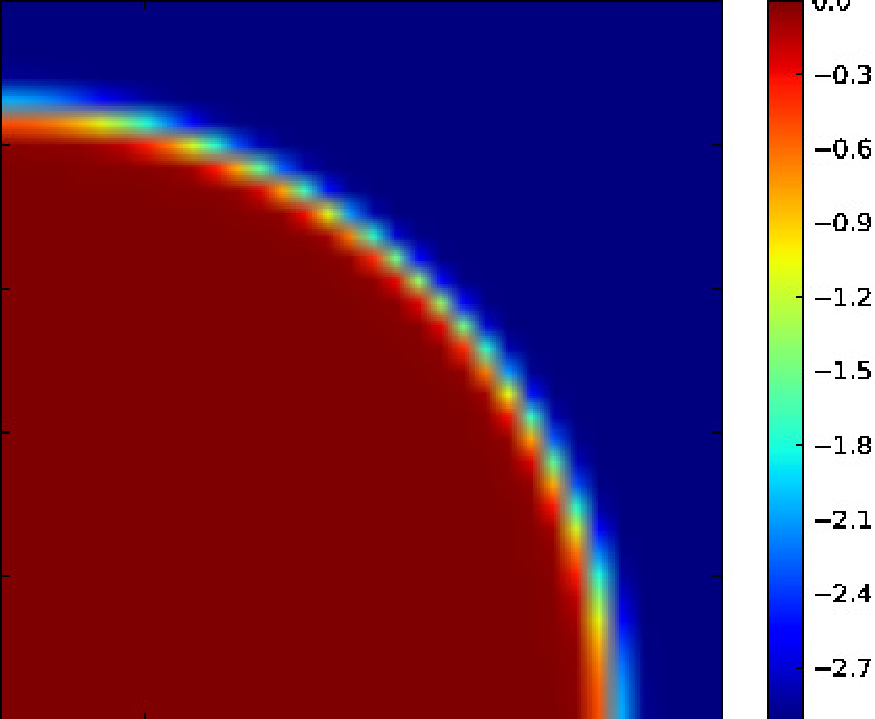
\includegraphics[scale=0.3]{i1-HIIcontour_500myr_nx32.pdf}
  \hfill}
\vspace{0.2cm}
\centerline{\hfill
  %% 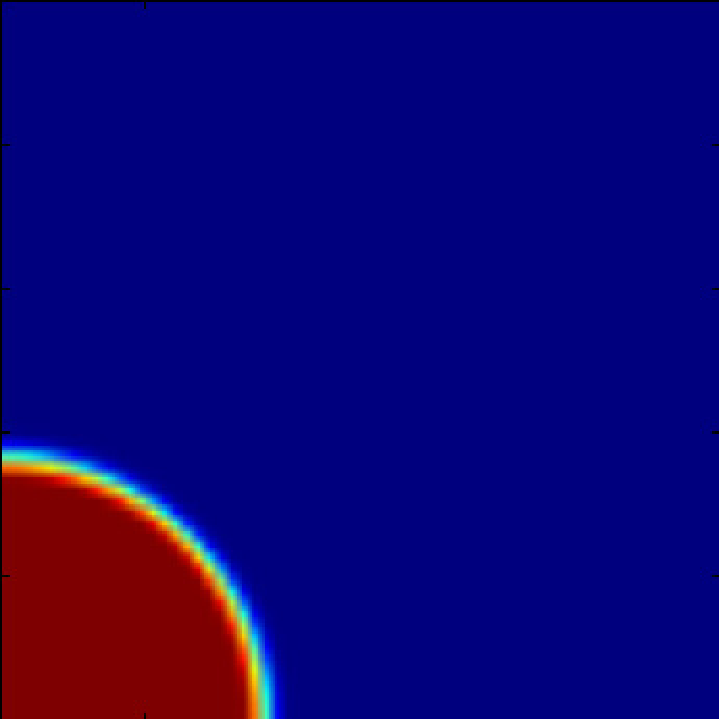
\includegraphics[scale=0.3]{i1-HIIcontour_10myr_nx64.eps}
  %% \hspace{0.1cm}
  %% 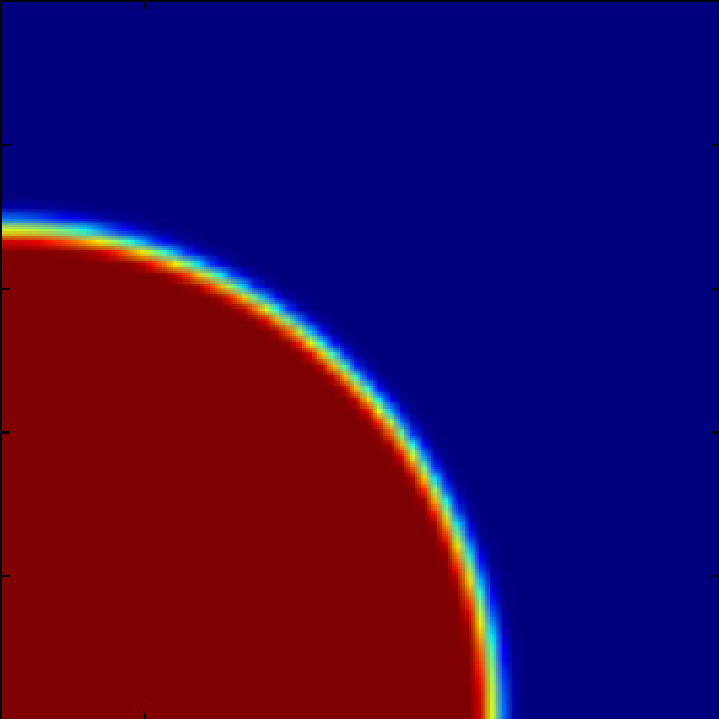
\includegraphics[scale=0.3]{i1-HIIcontour_100myr_nx64.eps}
  %% \hspace{0.1cm}
  %% 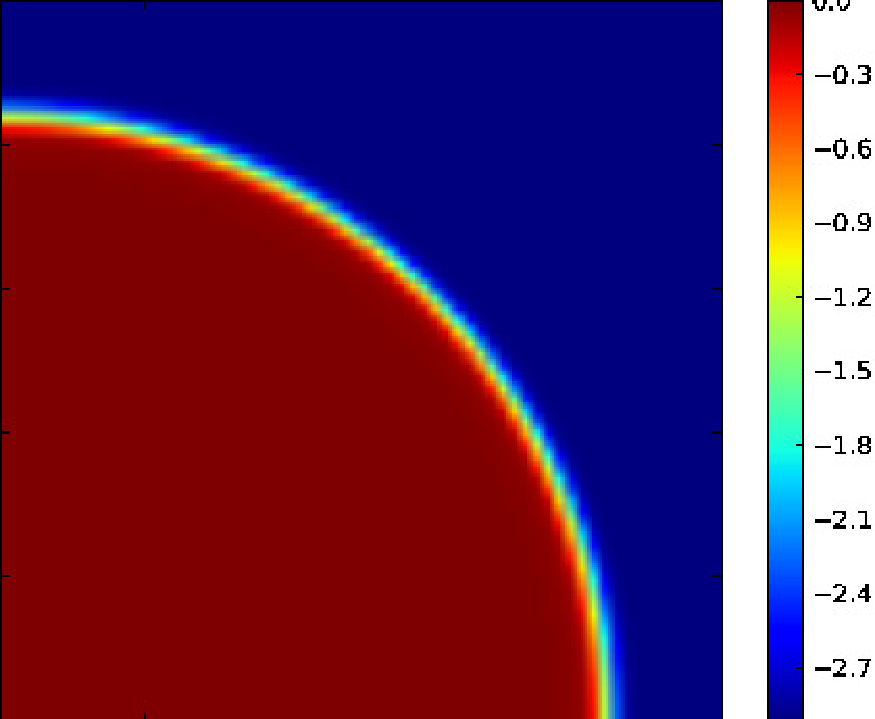
\includegraphics[scale=0.3]{i1-HIIcontour_500myr_nx64.eps}
  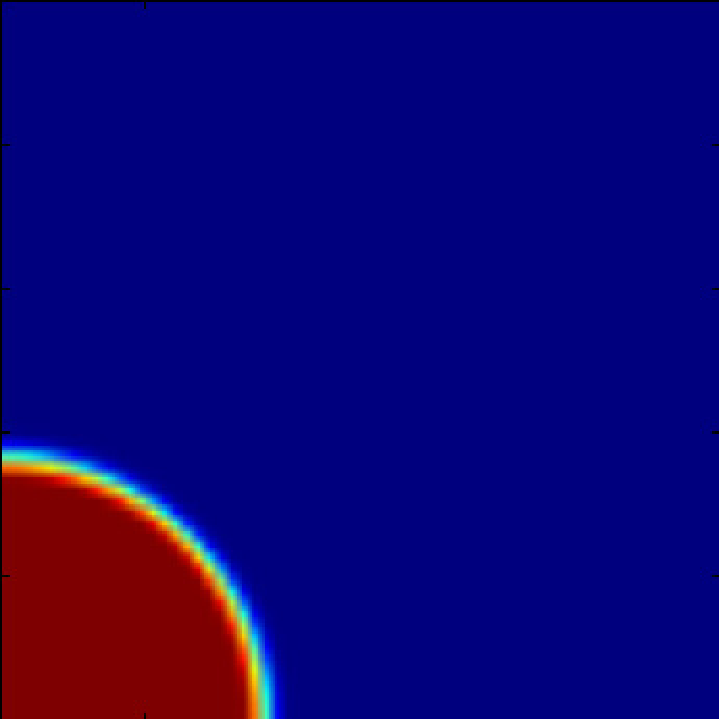
\includegraphics[scale=0.3]{i1-HIIcontour_10myr_nx64.pdf}
  \hspace{0.1cm}
  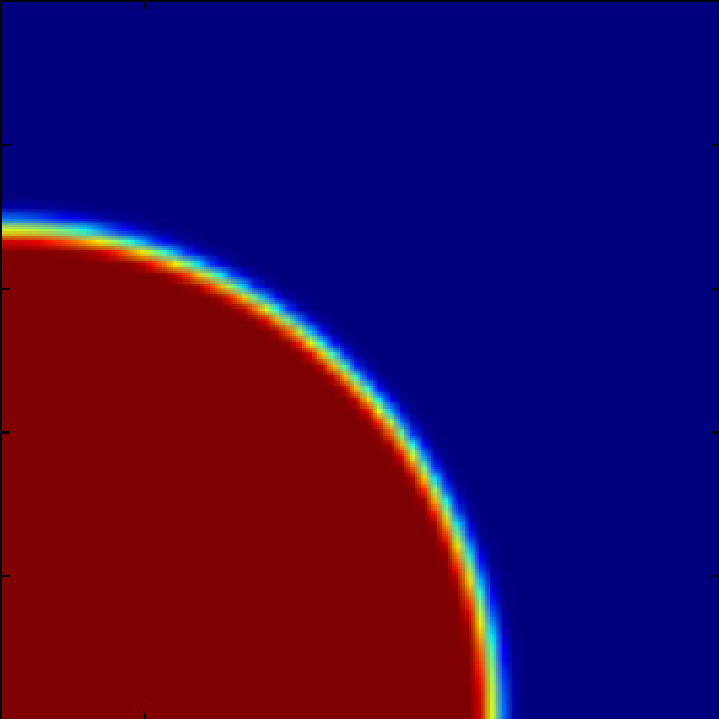
\includegraphics[scale=0.3]{i1-HIIcontour_100myr_nx64.pdf}
  \hspace{0.1cm}
  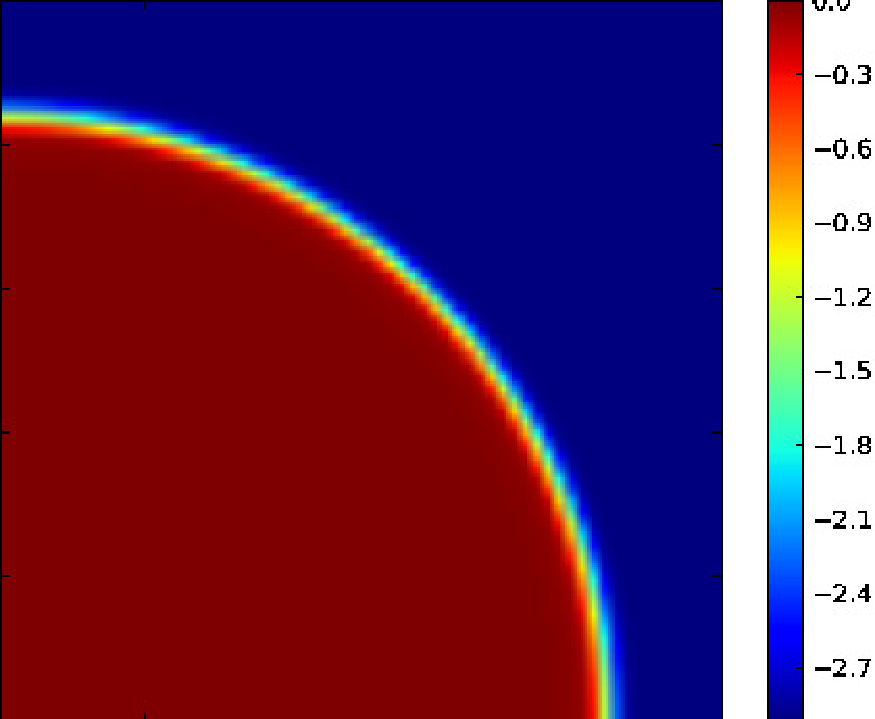
\includegraphics[scale=0.3]{i1-HIIcontour_500myr_nx64.pdf}
  \hfill}
\vspace{0.2cm}
\centerline{\hfill
  %% 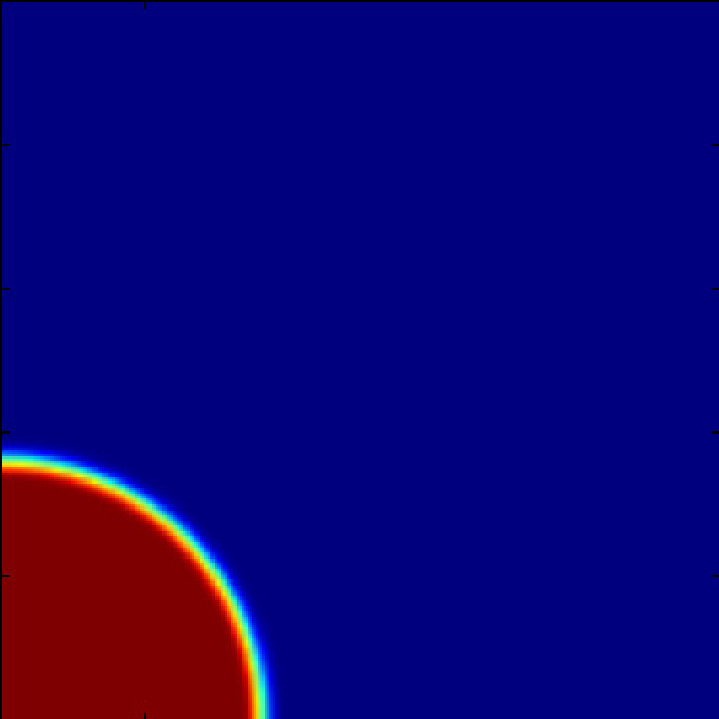
\includegraphics[scale=0.3]{i1-HIIcontour_10myr_nx128.eps}
  %% \hspace{0.1cm}
  %% 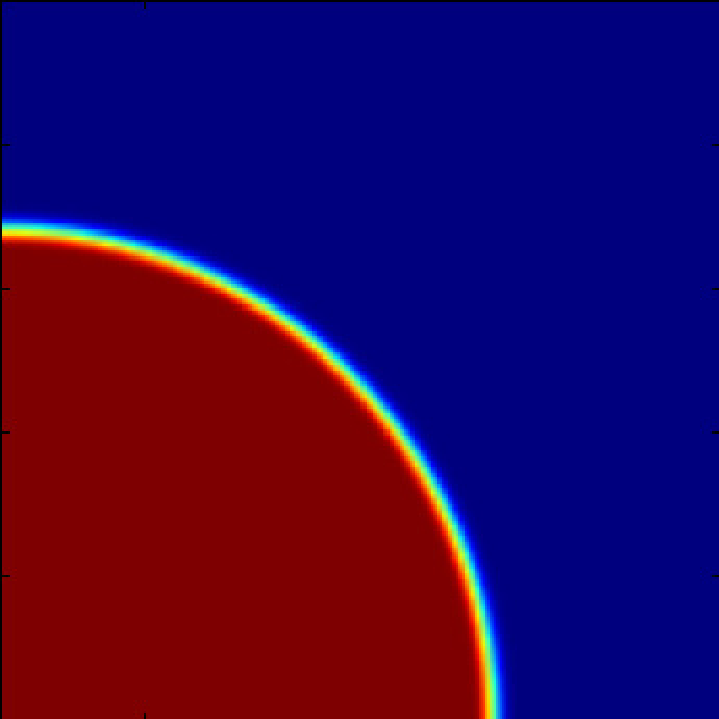
\includegraphics[scale=0.3]{i1-HIIcontour_100myr_nx128.eps}
  %% \hspace{0.1cm}
  %% 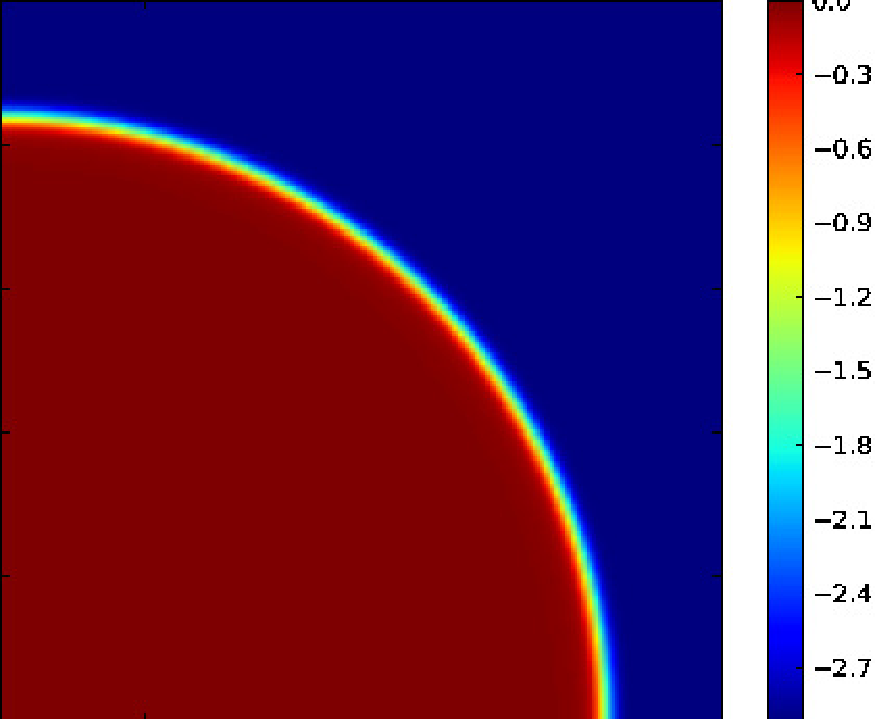
\includegraphics[scale=0.3]{i1-HIIcontour_500myr_nx128.eps}
  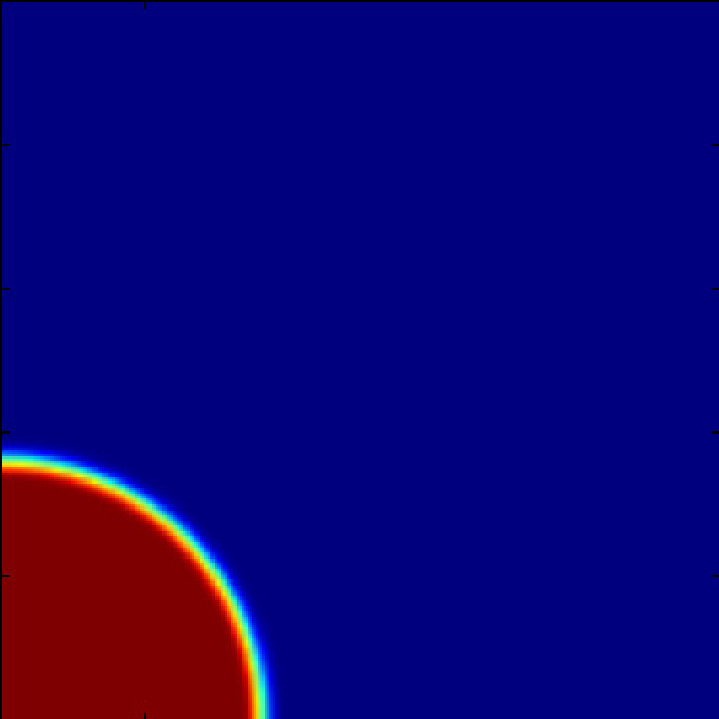
\includegraphics[scale=0.3]{i1-HIIcontour_10myr_nx128.pdf}
  \hspace{0.1cm}
  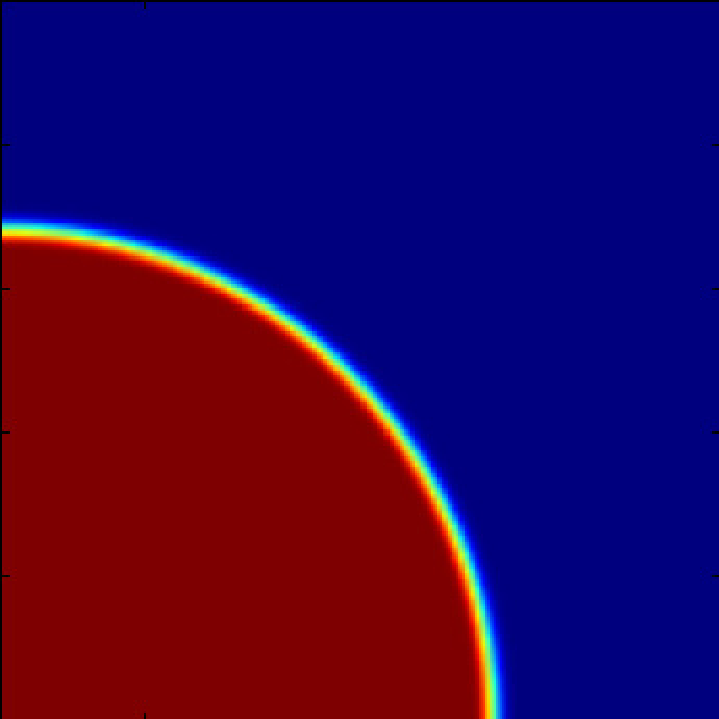
\includegraphics[scale=0.3]{i1-HIIcontour_100myr_nx128.pdf}
  \hspace{0.1cm}
  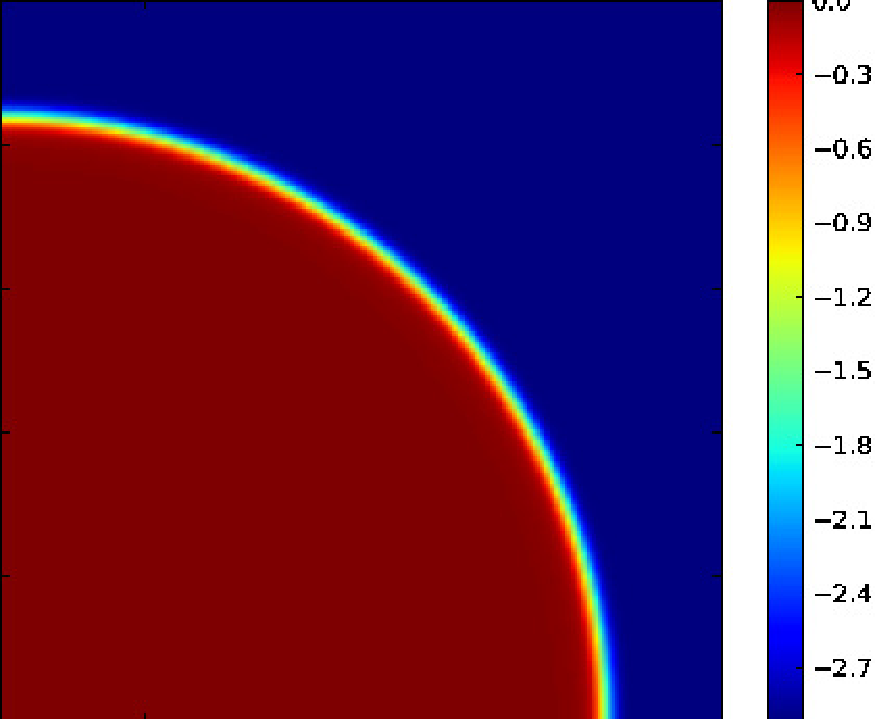
\includegraphics[scale=0.3]{i1-HIIcontour_500myr_nx128.pdf}
  \hfill}
  \caption{HII slices perpendicular to the $z$ axis (log$_{10}$
    scale).  We plot the evolution of the ionized region at times of
    10, 100 and 500 Myr (columns), and using spatial meshes of $16^3$,
    $32^3$, $64^3$ and $128^3$ (rows), to demonstrate the convergence
    to a spherical bubble.}
  \label{fig:i1_contours}
\end{figure}


\subsubsection{Cosmological radiative ionization}
\label{subsec:test2}

This verification test is a slight variation of the previous problem,
adding only the additional complication of a cosmologically expanding
universe.  Due to the cosmological expansion, the Str{\"o}mgren radius
itself increases due to the expansion of space, that reduces the
hydrogen number density $n_H$ as time proceeds,
\begin{equation}
  \label{eq:rs_cosmo}
  r_s(t) = \left(\frac{3\,\dot{N}_{\gamma}}{4\pi\,\alpha_B\,n_H(t)^2}\right)^{1/3}.
\end{equation}
This causes the I front to initially approach $r_s$, but eventually
fall behind as the expansion drives $r_s$ outward.  The analytical
solution to this problem is given by \cite{ShapiroGiroux1987},
\begin{align}
  \label{eq:radius_cosmo}
  r(t) &= r_{s,0} \left(\lambda e^{-\tau(a(t))} \int_{1}^{a(t)}
    e^{\tau(\tilde{a})}\left(1-2q_0+\frac{2q_0}{\tilde{a}}(1-z_0)\right)^{-1/2}\,\mathrm
    d\tilde{a} \right)^{1/3}, \\
  \notag \mbox{where} \qquad & \\
  \label{eq:tau}
  \tau(a) &= \lambda\left(F(a) - F(1)\right) \left(6q_0^2(1+z_0)^2\right)^{-1}, \\
  \label{eq:Fa}
  F(a) &= \left(2 - 4q_0 - \frac{2q_0}{a}(1+z_0)\right) 
     \left(1-2q_0+\frac{2q_0}{a}(1+z_0)\right)^{1/2}.
\end{align}
Here, the parameter $\lambda = \alpha_B n_{H,0} / H_0 / (1+z_0)$, with
$r_{s,0}$, $z_0$ and $n_{H,0}$ as the Str{\"o}mgren radius, redshift
and hydrogen number density at the beginning of the simulation.
Additionally, $q_0$ is the cosmological deceleration parameter, $H_0$
is the Hubble constant, and $a(t) = (1+z(t))^{-1}$ is the cosmological
expansion parameter. 

We run this problem using the parameters $q_0 = 0.5$, 
domain $[0,80\,\mbox{kpc}]^3$ (comoving), time/redshift domain $z =
[4,0]$, $H_0=0.5$, energy density contributions $\Omega_m = 1$,
$\Omega_A = 0$ and $\Omega_b = 0.2$.  Our initial conditions are $\rho
= 1.175\times 10^{-28}$ g cm$^{-3}$, $T = 10^4$ K and $E = 10^{-45}$
erg cm$^{-3}$.

We again plot spherically-averaged radial profiles of the radiation energy
density and the ionization fractions at redshifts 3.547, 2.423 and 1.692 from a
simulation using a 128$^3$ spatial grid and time step tolerance
$\tau_{tol} = 10^{-4}$ in Figure \ref{fig:sg_results}, showing the
expected propagation and eventual stalling of the radiation front and
resulting I-front in time.
\begin{figure}[t]
\centerline{\hfill
  %% 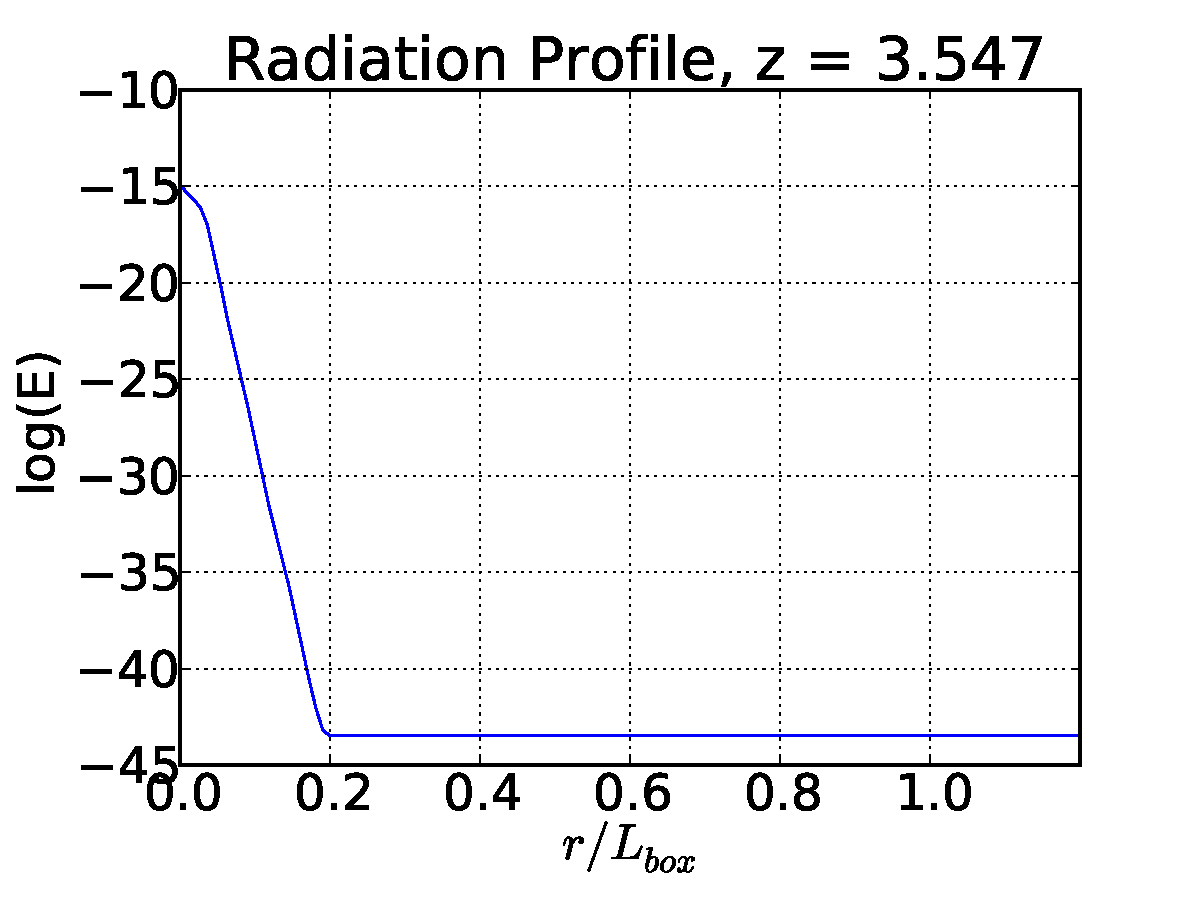
\includegraphics[scale=0.3, trim=1.0cm 0.5cm 1.0cm 0.5cm]{sg-Eprofiles_01.eps}
  %% 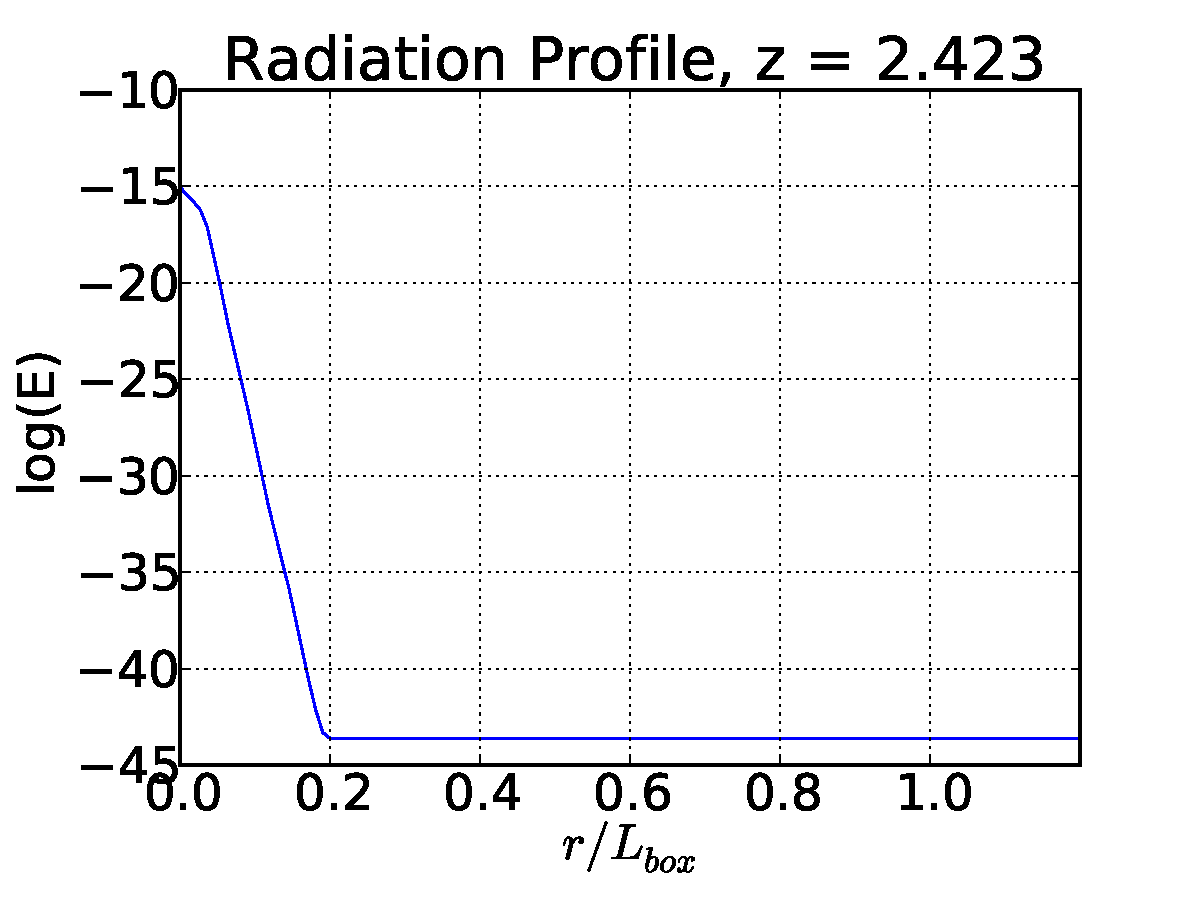
\includegraphics[scale=0.3, trim=1.0cm 0.5cm 1.0cm 0.5cm]{sg-Eprofiles_05.eps}
  %% 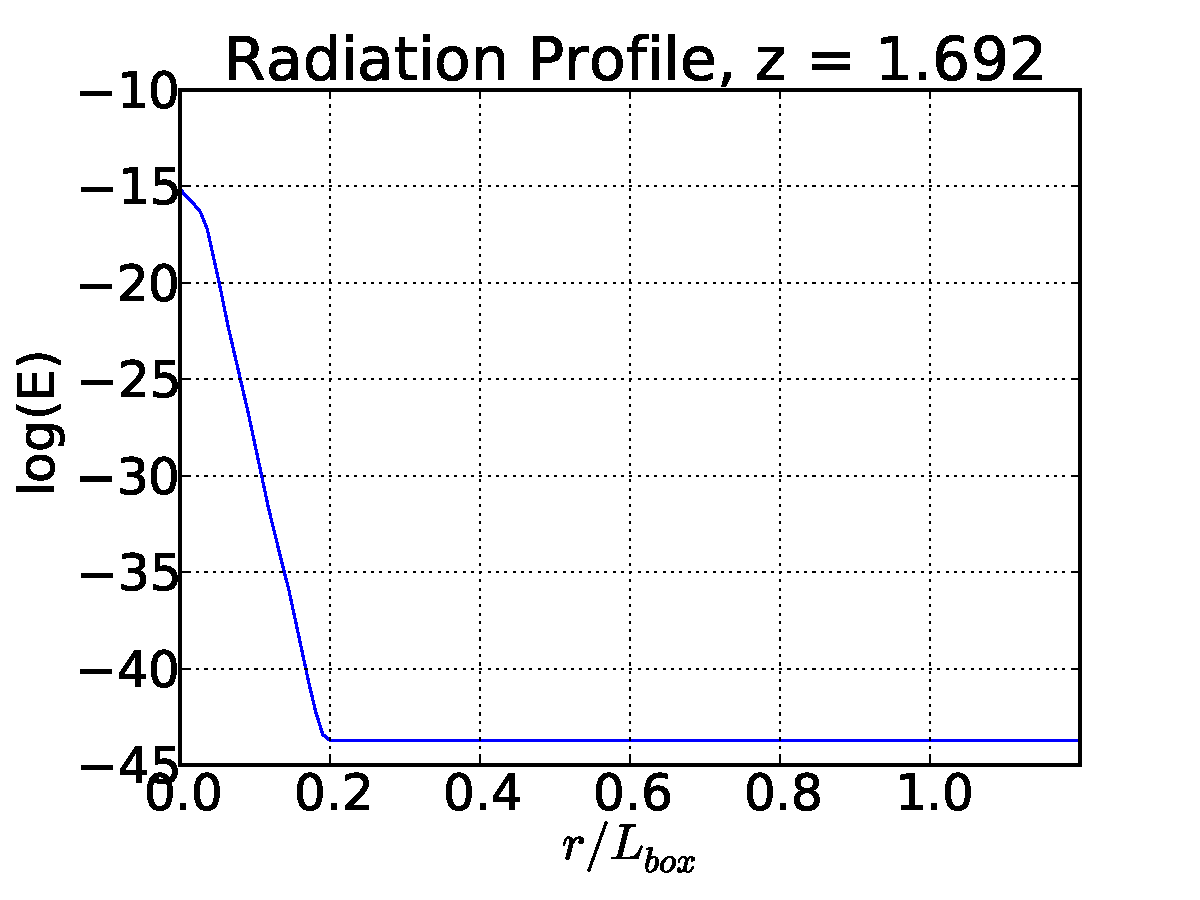
\includegraphics[scale=0.3, trim=1.0cm 0.5cm 1.0cm 0.5cm]{sg-Eprofiles_10.eps}
  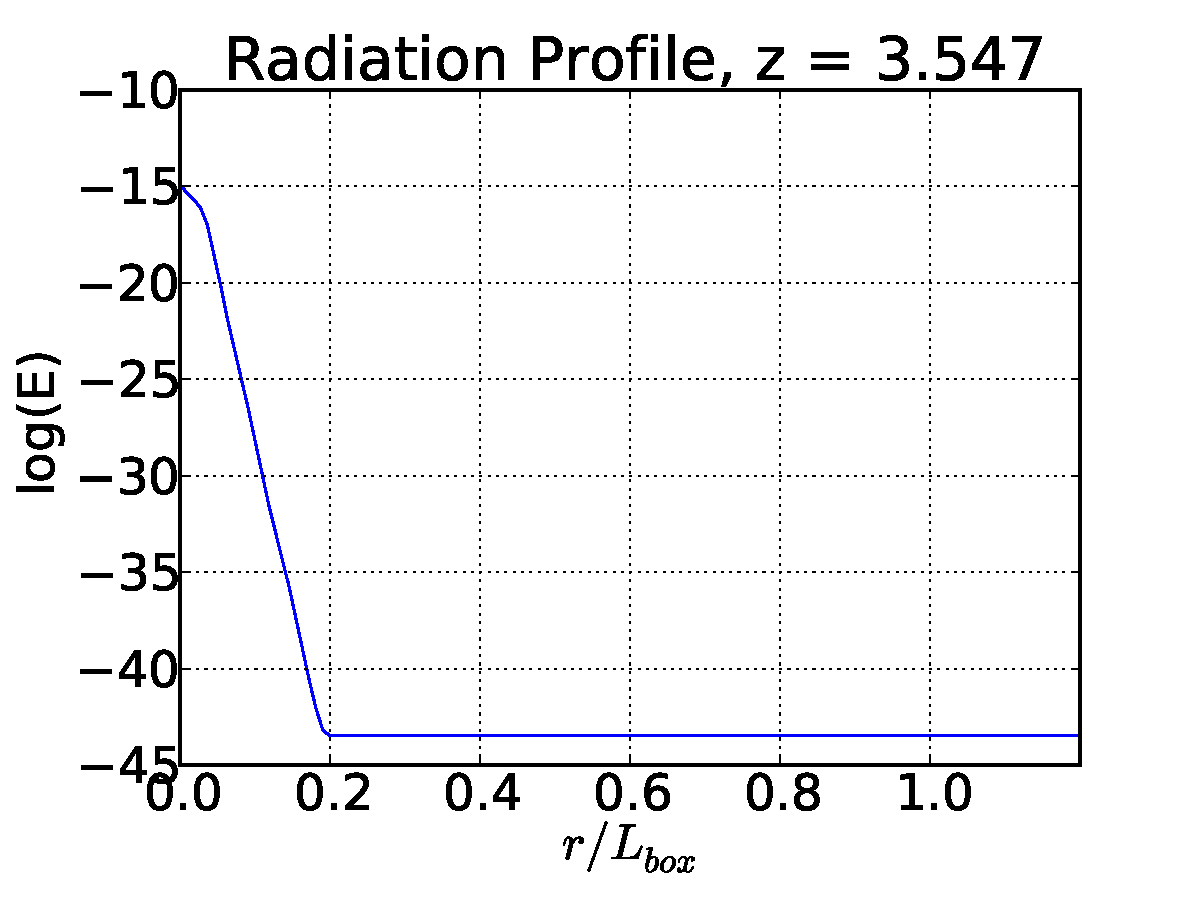
\includegraphics[scale=0.3, trim=1.0cm 1.0cm 1.0cm 0.5cm]{sg-Eprofiles_01.pdf}
  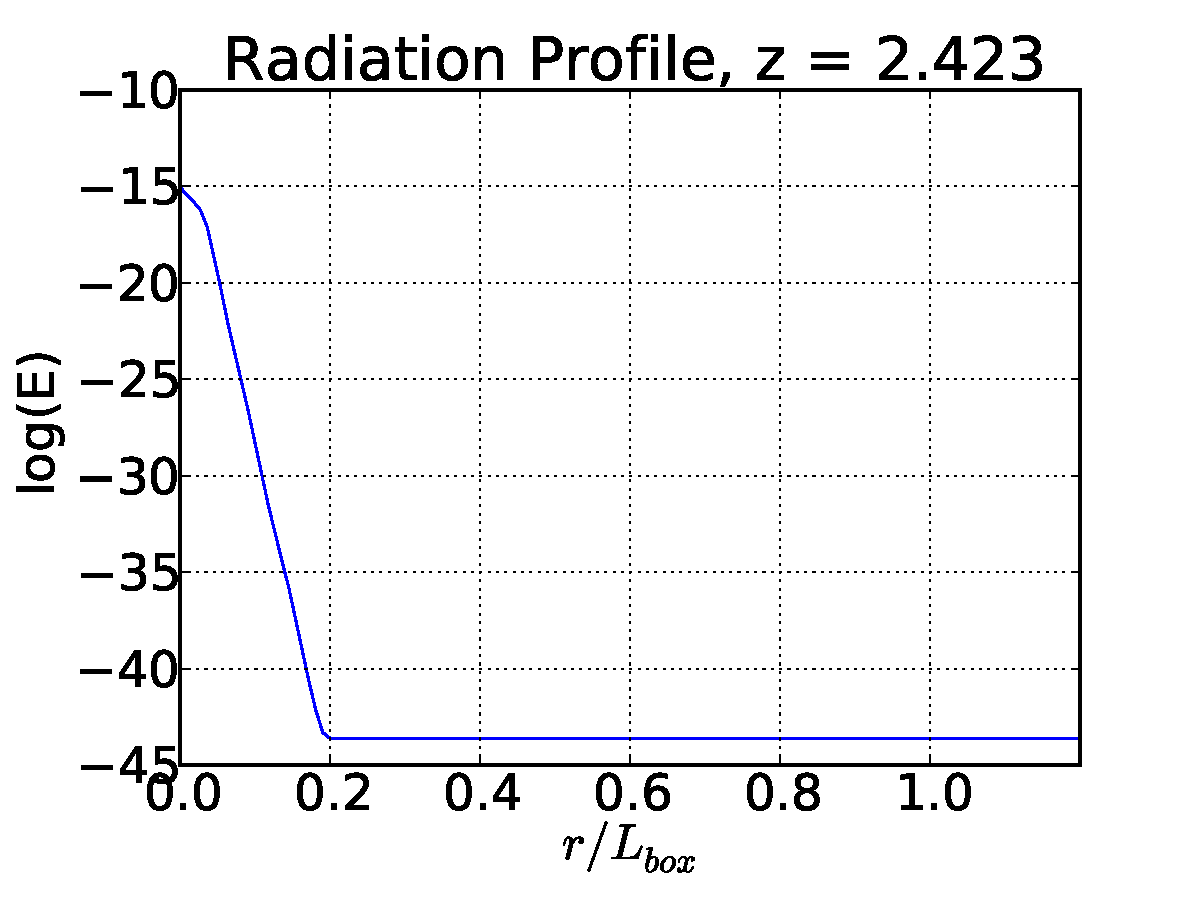
\includegraphics[scale=0.3, trim=1.0cm 1.0cm 1.0cm 0.5cm]{sg-Eprofiles_05.pdf}
  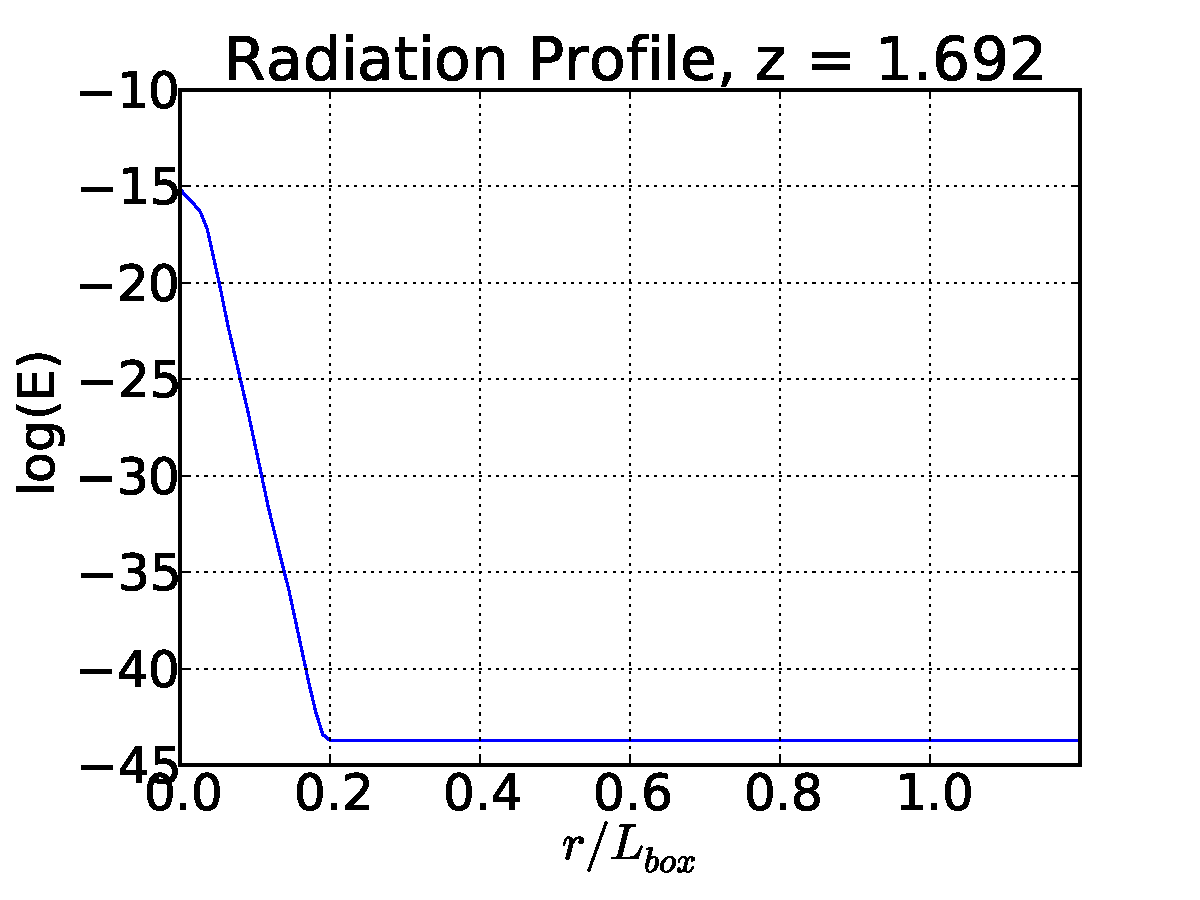
\includegraphics[scale=0.3, trim=1.0cm 1.0cm 1.0cm 0.5cm]{sg-Eprofiles_10.pdf}
  \hfill}
\centerline{\hfill
  %% \includegraphics[scale=0.3, trim=1.0cm 0.5cm 1.0cm 0.5cm]{sg-profiles_01.eps}
  %% \includegraphics[scale=0.3, trim=1.0cm 0.5cm 1.0cm 0.5cm]{sg-profiles_05.eps}
  %% \includegraphics[scale=0.3, trim=1.0cm 0.5cm 1.0cm 0.5cm]{sg-profiles_10.eps}
  \includegraphics[scale=0.3, trim=1.0cm 0.5cm 1.0cm 0.5cm]{sg-profiles_01.pdf}
  \includegraphics[scale=0.3, trim=1.0cm 0.5cm 1.0cm 0.5cm]{sg-profiles_05.pdf}
  \includegraphics[scale=0.3, trim=1.0cm 0.5cm 1.0cm 0.5cm]{sg-profiles_10.pdf}
  \hfill}
  \caption{Spherically-averaged radial profiles of radiation energy
    density and ionization fractions for the cosmological ionization
    test in section \ref{subsec:test2} using a $128^3$ mesh and
    time step tolerance $\tau_{tol} =10^{-4}$.  Plots are shown at z=3.547, 2.423 and 1.692
    (left to right), with the radiation energy density on
    the top row and ionization fractions on the bottom row.}
  \label{fig:sg_results}
\end{figure}
As with the previous test, we investigated the accuracy of our new
splitting approach between the radiation and chemistry solvers using
the same set of mesh sizes and time step tolerances as the test in
section \ref{subsec:test1}.  Figure \ref{fig:sg_stats} contains the
corresponding plots of the solution error and total runtime as a
function of the average time step size.  
\begin{figure}[t]
\centerline{\hfill
  %% \includegraphics[scale=0.45, trim=1.0cm 0.5cm 1.0cm 0.5cm]{sg-error_enzo.eps}
  %% \includegraphics[scale=0.45, trim=1.0cm 0.5cm 1.0cm 0.5cm]{sg-runtime_enzo.eps}
  \includegraphics[scale=0.45, trim=1.0cm 0.0cm 1.0cm 0.5cm]{sg-error_enzo.pdf}
  \includegraphics[scale=0.45, trim=1.0cm 0.0cm 1.0cm 0.5cm]{sg-runtime_enzo.pdf}
  \hfill}
  \caption{We ran tests using mesh sizes of
    $16^3$, $32^3$ and $64^4$, and time step tolerances of
    $10^{-2}$, $10^{-3}$, $10^{-4}$ and $10^{-5}$, and plot the I
    front position error as a function of the average time step size.
    As with Figure \ref{fig:i1_stats}, the runtime scales linearly
    with the inverse $\Delta t_{avg}$, and the error scales linearly
    with $\Delta t_{avg}$, at least until other sources of error
    dominate the calculation.} 
  \label{fig:sg_stats}
\end{figure}
Our results are similar to those from the previous test, indicating
that the modified time evolution approach employed in this work
successfully achieves accurate solutions of our coupled radiation and
ionization system.



\subsection{Validation Tests}
{\bf Validation tests are tests without analytic solutions that nonetheless serve as a
useful point of comparison between codes implementing different physical 
models and numerical methods \citep{IlievEtAl2006,IlievEtAl2009}. Our purpose is not to run all possible tests, but rather to validate the application of FLD to large scale reionization simulations, and in particular to investigate the well-known inability of FLD to cast a shadow on the general progress of reionization.
In this section we test our algorithm against 
four validation tests that are most relevant to the problem of cosmological 
reionization. The first two are radiation hydrodynamic tests studied by \cite{IlievEtAl2009} (hereafter RT09). They are the propagation of an I-front in a $r^{-2}$ density gradient, and the photoevaportion of a dense cloud irradiated from one side. The third validation test is the consolidated \hii region produced by two sources of equal luminosity introduced by \cite{Petkova09}. These three tests were chosen from a larger number of tests in the literature because they form a natural sequence with regard to the expansion and merging of isolated \hii regions in a clumpy IGM.  Finally, in a fourth test of our own design, we perform a direct comparison between FLD and ray tracing on a fully coupled reionization simulation in a small box. These tests demonstrate that although FLD ionizes dense clouds somewhat faster than methods that cast shadows, this affects primarily the earliest phases of cosmic reionzation when  a piece of neutral IGM is irradiated by the brightest nearby source. Later on, when multiple sources ionize the gas from multiple directions, FLD and ray tracing produce very similar evolutions. }    \st{To our knowledge these are the first FLD results
published to date, since the other codes running these problems have
focused on ray-tracing, Monte Carlo, and variable tensor Eddington
approximations of the radiative transfer equations.} 





\subsubsection{Test 6 -- I-front expansion in a $r^{-2}$ density profile}
\label{subsec:test6}

{\bf As our first validation test, we investigate Test 6 in
\cite{IlievEtAl2009} (hereafter RT09), that focuses on a full
radiation-hydrodynamics simulation of an ionized hydrogen (HII)
region in a spherically-symmetric density field.  Here, the center of
the region has constant number density, but at a specified core radius
$r_0$ the density rapidly decreases with radius.  Denoting this
functional relationship as $n_H(r)$, 
\[
   n_H(r) = \begin{cases}
     n_0,\quad&\text{for}\; r\le r_0\\
     n_0\left(\frac{r_0}{r}\right)^{2},\quad&\text{for}\; r> r_0.
   \end{cases}
\]
We follow the parameters choices from \cite{IlievEtAl2009}:  cubic
simulation domain of $[0,L]^3$ with $L=0.8$ kpc, core number density
$n_0 = 3.2$ cm$^{-3}$, core radius $r_0 = 91.5$ pc, zero initial
ionization fraction, ionization source at the origin with strength
$\dot{N}_{\gamma}=10^{50}$ photons s$^{-1}$ and a $T=10^5$ K blackbody
SED, initial temperature $T = 100$ K, reflective boundaries that touch
the origin and transmissive boundaries elsewhere, and a total
simulation time of $0\le t\le 25$ Myr.  Under these choices the
the I-front transitions from R-type to D-type within the core.  Once
the I-front reaches the beginning of the density gradient it begins to
accelerate, subsequently transitioning back to R-type.  Unfortunately,
for these simulation parameters, the problem exhibits no analytical
solution, so we refer to RT09 and WA11 for reference solutions to
compare against our own.

In the left half of Fig.~\ref{fig:test6_plots} we show time histories
of the I-front radius and velocity, that exhibit strong agreement with
the results from both RT09 and WA11.  In the right half of 
Fig.~\ref{fig:test6_plots} we plot radial profiles of the number
density, temperature, ionized fraction and pressure in the simulation
at 3, 10 and 25 Myr.  All of these results agree with reference
results from RT09 and WA11.  Perhaps the most notable difference may
be seen in the temperature and pressure profiles in comparison with
WA11, where our use of a grey approximation does not capture gas
preheating ahead of the I-front.

In Fig.~\ref{fig:test6_slices} we plot slices through the origin
of the ionized fraction, neutral fraction, temperature and number
density in the simulation at 25 Myr.  As it evident in these plots,
the FLD radiation approximation maintains a nearly spherical solution
profile throughout the simulation, with a slight anisotropy in the
non-coordinate aligned directions.  However, even with this minor
deviation of spherical symmetry, the results compare well against the
those in RT09 and WA11, many of which exhibit much more significant
anisotropy than that shown here. }



\begin{figure}[t]
\centerline{\hfill
  \includegraphics[scale=0.42, trim=0.0cm 0.0cm 0.0cm 0.0cm]{test6_radius.pdf}
  \includegraphics[scale=0.42, trim=0.0cm 0.0cm 0.0cm 0.0cm]{test6_profiles.pdf}
  \hfill}
  \caption{Test 6 (HII region in a $r^{-2}$ density profile).  Top
    left: growth of the computed I-front radius, computed as the
    radius with 50\% ionized fraction.  Bottom left: velocity of
    I-front radius, as computed from the upper plot at 0.5 Myr
    intervals.  Right: radial profiles at 3, 10 and 25 Myr, clockwise
    from top left as number density, temperature, pressure and Mach
    number.} 
  \label{fig:test6_plots}
\end{figure}

\begin{figure}[t]
\centerline{\hfill
  \includegraphics[scale=0.42, trim=0.0cm 0.0cm 0.0cm 0.0cm]{test6_slices.pdf}
  \hfill}
  \caption{Test 6 (HII region in a $r^{-2}$ density profile). Slices
    through the origin at 25 Myr.  Clockwise from top left: ionized
    fraction, Mach number, temperature and number density.}
  \label{fig:test6_slices}
\end{figure}






\subsubsection{Test 7 -- Photoevaporation of a dense clump}
\label{subsubsec:test7}
As our {\bf second} validation test we run Test 7 of RT09, and also studied by WA11 using {\em Enzo+Moray}. 
This is a radiation hydrodynamic test involving ionizing radiation impinging on a dense, opaque spherical cloud
which is subsequently photoevaporated. RT09 set this up as a plane wave of ionizing radiation sweeping over the 
cloud, {\bf whereas WA11 illuminated the cloud with a single point source whose luminosity was adjusted to produce the same ionizing flux at the cloud.} To facilitate comparison with the RT09 results, {\bf we implement the plane-wave illumination scheme, as described below} \st{we set it up as a spherical wave of ionizing radiation from
a point source sweeping over the cloud.} If run without hydrodynamics, the I-front is trapped in the dense cloud,
and the cloud casts a sharp shadow {\bf \citep{IlievEtAl2006}.  In reality, recombination radiation which would partially fill in the shadow zone, but this effect has not been included in validation tests to date. } With hydrodynamics engaged, the side of the cloud facing the source photoheats and expands, permitting a deeper
penetration of radiation into the cloud. Eventually, the entire cloud is photoevaporated. {\bf It is important to check
what FLD will do in this circumstance, in particular how the lack of a shadow affects the
photoevaporation time for the cloud.} \st{As we will now show, the effect is weak, validating our use of FLD for
large scale reionization problems.} 

The setup is as follows. A cubic domain 6.6 kpc on a side is employed, filled with an ambient medium of 
$n_H = 2 \times 10^{-4}$ cm$^{-3}$ and T=8000 K. The cloud is in pressure equilibrium with the intercloud
medium with density $n_H = 0.04$ cm$^{-3}$ and T=40 K. The cloud is a top-hat sphere with radius
$r_c$ = 0.8 kpc, and is centered at (x,y,z) = (5, 3.3, 3.3) kpc. The ionized fraction is initially zero everywhere. 
\st{A single radiation source is located in the center of the $x=0$ boundary. It has a luminosity of 
$\dot{N}_{\gamma}=3 \times 10^{51}$ photon/s.}
{\bf We implement the plane-wave illumination setup of RT09 by initializing an array of point sources on the left domain boundary, each emitting $10^6 A_{cell}$ ionizing photons/sec, where $A_{cell}$ is the area of the cell face. We have verified that this results in the correct flux of ionizing photons inside the domain.} \st{WA11 use the same four energy group spectral model to
represent a $10^5$ K blackbody as in Test 4 above. We use our grey FLD approximation which does not
model spectral hardening, as discussed above. We thus do not expect our results to be identical with WA11. }

Figs. \ref{fig:test7_slices_10} and \ref{fig:test7_slices_50}  shows slices through the cloud midplane of neutral fraction, pressure, temperature, and 
density at time $t=10, 50$ Myr, respectively. \st{At this time the I-front has propagated roughly 80\% through the cloud on the axis, compared to 
about 50\% in WA11. Because in the FLD approximation radiation propagates in the direction of the radiation energy density gradient,
it has filled in the  ``nightside" of the cloud, ionizing the cloud from all sides. By 10 Myr only a small neutral patch remains. 
Comparing with Fig. 27 
of WA11, we find similar structures on the ``dayside" of the cloud, but the complete absense of a neutral shadow on 
the nightside. }
{\bf By 10 Myr the cloud is fully ionized, whereas the results in RT09 show that the cloud is only partially ionized at this time. Inspection of Figs. 32 and 42 in RT09 suggest that the I front has only reached the center of the cloud after 10 Myr. The resolution of this discrepancy is that within the FLD approximation, the radiation quickly flows around the cloud, filling in the shadow region. The cloud is thus irradiated from all sides, not just one side. Therefore the time to ionize the cloud should be roughly the time it takes for the I-front to traverse a distance equal to the radius of the cloud. Ignoring attenuation, recombinations, and hydrodynamic effects the speed of the I-front in the dense gas is $v_{IF}=2.5 \times 10^7$ cm/s.  At this speed, it should take the I-front roughly 3.2 Myr to  reach the center of the cloud. }

{\bf In Fig. \ref{fig:time-evol} we plot the time evolution of the mass of \hi in the cloud. We see that the cloud becomes ionized on a timescale of about 5 Myr, somewhat longer than the estimate above. To improve on this estimate we ran a 1D version of the opaque cloud test. We placed a step function jump in density from $2 \times 10^{-4}$ cm$^{-3}$ to a value 200 times that at the center of the box; $x=3.3$ kpc. The position of the I-front versus time is shown in Fig. \ref{fig:box_wall_hydro-Ifront_history}. Including the attenuation of the ionizing flux, recombinations, and hydrodynamic motions, it takes the I-front about 5.8 Myr to propagate 0.8 kpc into the dense gas, in good agreement with Fig. \ref{fig:time-evol}.  }


%Fig. \ref{fig:test7_slices_50} shows the same information for the cloud at $t=50$ Myr.} 
By \st{this time} {\bf 50 Myr} the cloud has
expanded considerably and become completely ionized, exhibiting a roughly spherical shape. 
The results of {\bf RT09 and} WA11 are similar, except for a small wedge-shaped neutral patch on the back of the cloud, which casts 
a small shadow into the diffuse intercloud medium. 
In reality, ionizing recombination radiation from the denser cloud gas would fill in this shadow and ionize the 
diffuse gas there, making it more like the FLD solution. 

To enable a more quantitative comparison with {\bf RT09 and}  WA11,
we plot in Fig. \ref{fig:test7_profiles} line cuts from the point source through the center of the cloud at
$t=1, 10, 50$ Myr. 
Because the FLD method ionizes the cloud from all sides with only a small delay between
dayside and nightside irradiation, we see a less pronounced dayside-nightside asymmetry in the density and neutral fraction 
profiles compared with WA11 at 10 and 50 Myr. Both methods show good agreement on the position and structure
of the dense shell swept up by the expanding cloud at 50 Myr at $x/L_{box} \sim 0.4$. 
Significant differences are seen at 50 Myr for $x/L_{box} > 0.75$ (the cloud's center) due to shadowing effects in the {\em Moray} result
which is absent in the FLD result.  

{\bf Fig. \ref{fig:box_wall_hydro-profiles} plots the same quantities for the 1D test problem introduced above. These profiles look very much like the results of the 3D methods that cast shadows in RT09 and WA11. In particular, we see in the neutral fraction plot that at $t=10$ Myr, the I-front has propagated a distance of $x/L_{box} \approx 0.16 $ (1 kpc) into the dense material, similar to the 3D results in RT09 and WA11. Likewise, at $t=50$ Myr, the I-front has propagated a distance of $x/L_{box} \approx 0.3 $ (2 kpc) into the dense material, which is slightly larger than the diameter of the cloud in Test 7. } 

Overall, the FLD calculation ionizes the cloud \st{somewhat} faster than predicted by WA11. However by 50 Myr both calculations
produce a cloud which is either fully ionized or nearly so, and there is good agreement on the size of the {\bf expanding} cloud.  
The most significant difference is that the ray-tracing calculation predicts a small, neutral wedge-shaped patch on the nightside
of the cloud which is absent in the FLD calculation. It is unlikely that this difference will be important in large scale reionzation
simulations since clouds will be irradiated from multiple directions during the overlap phase. 


\begin{figure}[t]
\centerline{\hfill
  %% \includegraphics[width=0.75\textwidth]{test7_slices_K.eps}
  \includegraphics[width=0.75\textwidth]{test7_slices_K.pdf}
  \hfill}
  \caption{Test 7. Photo-evaporation of a dense clump. Clockwise from upper left: Slices through the clump midplane of neutral fraction, pressure, temperature, and density at time $t=10$ Myr.}
  \label{fig:test7_slices_10}
\end{figure}

\begin{figure}[t]
\centerline{\hfill
  %% \includegraphics[width=0.75\textwidth]{test7_slices_K2.eps}
  \includegraphics[width=0.75\textwidth]{test7_slices_K2.pdf}
  \hfill}
  \caption{Test 7. Photo-evaporation of a dense clump. Same as Fig. \ref{fig:test7_slices_10} at time $t=50$ Myr.}
  \label{fig:test7_slices_50}
\end{figure}

\begin{figure}[t]
\centerline{\hfill
  %% \includegraphics[scale=0.6, trim=1.0cm 0.5cm 1.0cm 0.5cm]{test7_profiles_K.eps}
  \includegraphics[scale=0.6, trim=1.0cm 0.5cm 1.0cm 0.5cm]{test7_profiles_K.pdf}
  \hfill}
  \caption{Test 7. Photo-evaporation of a dense clump. Line cuts through the center of the cloud at $t=1, 10, 50$ Myr for (clockwise from upper left) density, temperature, pressure, and neutral fraction. }
  \label{fig:test7_profiles}
\end{figure}

\begin{figure}[t]
\centerline{\hfill
  \includegraphics[width=0.7\textwidth]{test7_ionization_history2.pdf}
  \hfill}
  \caption{Test 7. Time evolution of the mass of hydrogen in the cloud ionized to more than 10\% (solid line) and 90\% (dashed line). }
  \label{fig:time-evol}
\end{figure}

\begin{figure}[t]
\centerline{\hfill
  \includegraphics[width=0.7\textwidth]{box_wall_hydro-Ifront_history.pdf}
  \hfill}
  \caption{I-front position vs. time in the 1D test problem described in the text. Including flux attenuation, recombinations, and hydrodynamic effects, the I-front takes roughly 5.8 Myr to propagate a distance $d=0.8$ kpc in the dense gas. }
  \label{fig:box_wall_hydro-Ifront_history}
\end{figure}

\begin{figure}[t]
\centerline{\hfill
  \includegraphics[width=0.7\textwidth]{box_wall_hydro-profiles.pdf}
  \hfill}
  \caption{Plots of density, temperature, pressure, and neutral fraction at $t=1, 10, 50$ Myr for the 1D step function test problem described in the text.}
  \label{fig:box_wall_hydro-profiles}
\end{figure}

\subsubsection{Consolidated HII region with two sources}
As our last validation test we demonstrate the performance of our FLD radiative transfer method on a consolidated \hii region with two nearby point sources of equal luminosity. This problem was introduced by Petkova \& Springel (2009) (hereafter PS09) and included in the extensive suite of tests carried out by WA11. This is a validation problem because it has no analytic solution (that we know of.) PS09 studied it because their method uses the variable tensor Eddington factor moment method \citep{StoneMihalasNorman92,NormanAbelPaschos98,HayesNorman2003}  where the Eddington tensor is computed assuming the medium is optically thin everywhere \citep{GnedinAbel2001}. As discussed in \cite{GnedinAbel2001} it is known that the shapes of consolidated \hii regions are slightly inaccurate due to the optically thin assumption, in the sense that the \hii region is  more elongated in the axial direction, and less expanded in the transverse direction than in reality. 
The solution presented by PS09 shows this elongation. The solution presented
in WA11, which shows rounder but still slightly elongated I-fronts, should be a closer approximation to truth since it is calculated using adaptive
ray tracing which in principle gets the geometric effects correct. However the omission of 
diffuse ionizing recombination radiation which becomes dominant near a stalled I-front
means that even the WA11 solution is an approximation to the true shape. It is thus interesting
to see what FLD produces for this problem. 

The setup is as follows. Two sources with luminosities of $5 \times 10^{48}$ photons/s
are separated by 8 kpc. The ambient medium is static with uniform density $10^{-3}$
cm$^{-3}$ and T = $10^4$ K. The computational domain is 20 kpc in width and 10 kpc
in height and depth, and resolved with mesh of $128 \times 64 \times 64$ cells. The 
problem is evolved for 500 Myr, which is long enough for the consolidated HII region to
evolve to a steady state. 

Fig. \ref{fig:consolidated} shows slices of neutral fraction on $x-y$ and $x-z$ planes 
through the axis connecting the sources. The consolidated
\hii region is similar in size to the solution presented by WA11, but noticeably rounder
near its extremities. We do not include diffuse ionizing recombination radiation in our
formalism, and thus this must be a consequence of FLD. Since we are solving the same
problem, we expect the WA11 solution is closer to the truth, but note that the FLD solution is an acceptable approximation to truth given our intended application to large scale reionization. 


\begin{figure}[t]
\centerline{\hfill
  %% \includegraphics[width=0.75\textwidth]{consolidated.eps}
  \includegraphics[width=0.75\textwidth]{consolidated.pdf}
  \hfill}
  \caption{Consolidated HII region test - slices of the neutral fraction through the $x-y$ and $x-z$ planes at $t=500$ Myr.}
  \label{fig:consolidated}
\end{figure}

\subsubsection{Comparing FLD and Ray Tracing on a Cosmological Reionization Test Problem}
{\bf In  Paper II we introduced a new test problem to directly compare the results of Enzo's adaptive ray tracing scheme {\em Moray} with FLD in order to assess the importance of shadowing. We examined the evolution of the ionized hydrogen volume and mass fractions in a fully-coupled cosmological reionization simulation in a 6.4 comoving Mpc box. We also examined PDFs of temperature and ionization fraction as a function of baryon overdensity. We showed that while FLD ionizes somewhat faster than ray tracing at early times ($Q_{\hii}<<1$), the late time evolutions are very similar. We hypothesized that the reason for this is that early times, shadowing is more important since opaque clouds are primarily irradiated by a single dominant source driving the expansion of isolated \hii regions. At late times, as the ionized volume fraction approachs unity, a given opaque neutral cloud will be irradiated from multiple directions--a situation that FLD approximates well. Here we present additional analysis. 

The test problem is a scaled down version of the 20 Mpc simulation described in Paper II. It is identical in physics model, mass resolution, and spatial resolution, but is in a volume $(20/6.4)^3 \approx 30\times$ smaller. The simulation is carried out on a uniform mesh of $256^3$ grid cells and an equal number of dark matter particles. The reader is referred to Paper II for additional details.

In Fig. \ref{fig:ionization_evolution} we plot the evolution of the ionized hydrogen volume and mass fractions for the {\em Moray} simulation, and three FLD simulations differing in the choice for the radiation transport timestep control factor $\tau_{tol} = 10^{-2}, 10^{-3}, 10^{-4}.$ Note that the sampling intervals are different for each simulation, which accounts for the jagged FLD curves. For a smoother representation for the $\tau_{tol} = 10^{-3}$ case see Figure 32 in Paper II. Generally we see that the FLD simulations ionize slightly faster than the ray tracing simulation, with this being more evident in the mass-weighted curves as compared with the volume-weighted curves. This is qualitatively what we would expect given the results of the Test 7 described above, wherein we showed that FLD completely ionizes an opaque cloud irradiated from one side whereas ray tracing leaves a small neutral patch on the ``nightside" of the cloud. 

Figures \ref{fig:FLD_Moray_z10}, \ref{fig:FLD_Moray_z9}, and \ref{fig:FLD_Moray_z8} show projections through the box of the density-weighted electron fraction and gas temperature for the FLD and ray tracing simulations at three redshifts: $z=10, 9, 8$. Overall, we see very good correspondance between ionized regions at all redshifts. The one noticeable difference is the smoothness of the FLD I fronts versus the jaggedness of the ray tracing I fronts. Without further detailed study we cannot say whether this difference is the result of shadowing, ray discreteness effects, or a manifiestation of I front instabilities \citep{WhalenNorman2008a,WhalenNorman2008b,WhalenNorman2011}. 

Finally we show in Figure \ref{fig:ionized_DFs} distribution functions of ionized hydrogen versus baryon overdensity for the FLD ($\tau_{tol}=10^{-3}$) and ray-tracing simulations at $z=8$. Figure \ref{fig:ionized_DFs}a plots the total mass of \hii versus overdensity. We see than FLD ionizes about 10\% more gas at mean density and above compared to ray tracing.   Figure \ref{fig:ionized_DFs}b plots the normalized mass of \hii versus overdensity. This scales out the total mass and allows us to see how the ionized gas is distributed at various overdensities. The two distribution functions agree at $\log (\Delta_b) < -0.5$ and $\log (\Delta_b) > 2$. However in the intermediate regime $-0.5 \leq \log (\Delta_b) \leq 2$ we see that FLD has somewhat less gas at near mean density relative t ray tracing, consistent the greater ionized volume fraction, and has somewhat more gas with overdensities of $\sim 10$ in the (partially) ionized state.  This is consistent with the interpretation stated above and discussed in more detail in Paper II that gas of moderate overdensities is over-ionized relative to ray tracing at the level of about 10\%. We expect this number to be resolution-dependent, and are in the process of doing a resolution study on this problem to see if convergence can be achieved at higher resolution. }

\begin{figure}[t]
\centerline{\hfill
  \includegraphics[width=0.5\textwidth]{compareIonized_vs_Redshift_10.pdf}
  \includegraphics[width=0.5\textwidth]{compare_mw_Ionized_vs_Redshift.pdf}
  \hfill}
  \caption{Comparing FLD and ray tracing solutions on a cosmological reionization test problem. (a) evolution of ionized hydrogen volume fraction, and (b) evolution of ionized hydrogen mass fraction for gas that is at least 10\% ionized. In each figure we plot the {\em Moray} curve and three curves from FLD simulations with three different radiation timestep tolerance parameters $\tau_{tol}$. Note that the sampling intervals are different for each simulation, which accounts for the jagged FLD curves. For a smoother representation, see Figure 32 in Paper II.}
  \label{fig:ionization_evolution}
\end{figure}

\begin{figure}[t]
\centerline{\hfill 
  \includegraphics[width=0.5\textwidth]{proj_Electron_Fraction_wDensity_x_RD0001.pdf}
  \includegraphics[width=0.5\textwidth]{proj_Electron_Fraction_wDensity_x_RedshiftOutput0003.pdf}
  \hfill}
  \centerline{\hfill
  \includegraphics[width=0.5\textwidth]{proj_Temperature_wDensity_x_RD0001.pdf}
  \includegraphics[width=0.5\textwidth]{proj_Temperature_wDensity_x_RedshiftOutput0003.pdf}
  \hfill}
  \caption{Comparing FLD and ray tracing solutions on a cosmological reionization test problem. Shown are projections of density-weighted electron fraction (top row) and temperature (bottom row) for FLD (left column) and {\em Moray} adaptive ray tracing solutions (right column). Results are shown for $z=10$.}
  \label{fig:FLD_Moray_z10}
\end{figure}

\begin{figure}[t]
\centerline{\hfill
  \includegraphics[width=0.5\textwidth]{proj_Electron_Fraction_wDensity_x_RD0002.pdf}
  \includegraphics[width=0.5\textwidth]{proj_Electron_Fraction_wDensity_x_RedshiftOutput0004.pdf}
  \hfill}
\centerline{\hfill
  \includegraphics[width=0.5\textwidth]{proj_Temperature_wDensity_x_RD0002.pdf}
  \includegraphics[width=0.5\textwidth]{proj_Temperature_wDensity_x_RedshiftOutput0004.pdf}
  \hfill}
  \caption{ Same as Fig. \ref{fig:FLD_Moray_z10} except for $z=9$.}
  \label{fig:FLD_Moray_z9}
\end{figure}

\begin{figure}[t]
\centerline{\hfill
  \includegraphics[width=0.5\textwidth]{proj_Electron_Fraction_wDensity_x_RD0003.pdf}
  \includegraphics[width=0.5\textwidth]{proj_Electron_Fraction_wDensity_x_RedshiftOutput0005.pdf}
  \hfill}
\centerline{\hfill
  \includegraphics[width=0.5\textwidth]{proj_Temperature_wDensity_x_RD0003.pdf}
  \includegraphics[width=0.5\textwidth]{proj_Temperature_wDensity_x_RedshiftOutput0005.pdf}
  \hfill}
  \caption{Same as Fig. \ref{fig:FLD_Moray_z10} except for $z=8$.}
  \label{fig:FLD_Moray_z8}
\end{figure}


\begin{figure}[t]
\centerline{\hfill
  \includegraphics[width=0.5\textwidth]{ionized_histogram.pdf}
  \includegraphics[width=0.5\textwidth]{normalized_histogram.pdf}
  \hfill}
  \caption{Distribution functions of ionized hydrogen versus baryon overdensity for the FLD and ray-tracing simulations at $z=8$. (a) total mass of \hii; (b) normailized mass of \hii .}
  \label{fig:ionized_DFs}
\end{figure}


\subsection{Parallel Scalability}
\label{subsec:scalability}

%Weak scaling: Figure 6 from the INCITE renewal proposal.

\st{Excellent scalability of our radiation diffusion solver is fundamentally important to being 
able to simulate reionization in large cosmological volumes. Once the 
mass and spatial resolution requirements are established to adequately model the 
smallest galaxies in the source population, the problem becomes one of ``weak
scaling"; i.e., increasing the simulated volume at fixed resolution, rather than increasing
the resolution in a fixed volume. To test the scaling of our solver, we create a 3D cubic array
of isothermal Str\"{o}mgren sphere test problems as described in Sec. 4.1.1, each resolved by a $64^3$ cell subvolume of the global mesh. A point source is placed in the center of each
subvolume.  Each subvolume is assigned to
an MPI task which is in turn executed on one core of the Cray XT5 machine ``Kraken"
operated by the National Institute for Computational Science (NICS) at ORNL. 
Thus a simulation with $P^3$ point sources is simulated with a global
mesh of dimension $(64P)^3$ cells, and executes on $P^3$ cores.}

\st{ Fig. 20 shows the weak scaling results for P=2, 4, 8, 16, 32, corresponding to meshes of size $128^3$, $256^3$, $512^3$, $1024^3$, and $2048^3$ cells. We see that logarithmic scaling is achieved to at least 32,768 MPI tasks (and point sources) on a $2048^3$ test problem with $64^3$ tiles. This is the expected optimal scaling results, which reflects the scalability of the {\em hypre} geometric multigrid routines used to solve the linear system of equations resulting from the discretization and linearization of the FLD equation. }

{\bf Our numerical method is highly scalable. The scalability of the radiation diffusion solver has already been presented in \cite{ReynoldsHayesPaschosNorman2009}. There we show that our geometric multigrid--based solver exhibits the expected $\log p$ scaling on an idealized weak scaling test involving an array of ionizing point sources. 

More interesting and relevant is the weak scaling of the entire reionization computation combining dynamics, gravity, and radiation transport. This is the regime relevant to cosmic reionization. The weak scaling of our combined calculation can be illustrated very straight-forwardly. We have performed two fully-coupled reionization simulations differing only in the box size. One is performed in a volume 20 comoving Mpc on a side resolved by $800^3$ cells and dark matter particles \citep{So2014}. The other, described below, is performed in a volume 80 comoving Mpc on a side, resolved by $3200^3$ cells and dark matter particles. The larger simulation is 64 times the volume of the smaller simulation, but is computed using 64 times as many cells and particles. Thus, the mass and spatial resolutions are identical. Both simulations were computed on Cray XT5 systems at ORNL with identical node designs and interconnects. The compute nodes had dual hex-core AMD Operton processors with 16 GB RAM and a clock speed of 2.6 GHz. The smaller simulation was computed on 512 cores, and consumed 255,000 core-hrs. The larger simulation was computed on 31,250 cores and consumed 38,000,000 core-hrs. Since the execution time is dominated by the radiation diffusion solver, and this uses a multigrid solver with demonstrated $\log p$ scaling, the ratio of costs would be predicted to be 255,000 core $\times 64 \log (31,250) / \log(512) = 27.2$M core-hrs. Our large simulation is thus running at 72\% parallel efficiency relative to the small simulation. The origin of this inefficiency is the lack of particle load-balancing among the processors, as well as the global gravity solve which is performed using less than optimal FFTs at this scale. }

\subsection{Execution Speed Tests: Hydro vs. Rad-Hydro}
\label{subsec:speed}

Here we examine the relative execution speed between a pair of {\em Enzo} cosmological simulations with and without
FLD radiative transfer engaged, henceforth referred to as RHD and HD models, respectively. The RHD model is a simulation of
inhomogeneous cosmic reionization in a 80 Mpc comoving volume resolved by a uniform mesh of $3200^3$ cells and the same
number of dark matter particles. The problem is partitioned into $25^3 = 15,625$ MPI tasks, each of which evolves
a $128^3$ tile of the global mesh and is assigned to a different processor core. The physics model is as described in Sec. 2. 
The RHD model includes star formation and feedback (radiative, thermal, and chemical) as described in Sec. \ref{subsec:starform},
FLD radiative transfer, and 6-species primordial gas chemistry and ionization. 
The simulation was
carried out on the Cray XT5 supercomputer architecture {\em ORNL Jaguar}. The HD model is identical in all 
respects to the RHD model except that the FLD solver is not called each timestep. The HD simulation corresponds
to a primordial  6-species hydro-cosmological simulation with star formation and supernova feedback which is similar in
all respects to a standard Lyman alpha forest simulation in which the IGM is ionized by a homogeneous UV 
background, treated in the optically thin limit (e.g., \citet{Jena05}). 

Fig. \ref{fig:logcost} shows the cumulative wall time per core for the HD and RHD models plotted as a function of 1/z. 
The inflection in the curves at 1/z $\approx 0.07$ corresponds with the onset of star formation at z=14. Subsequently 
hot $10^6-10^7$ K gas is produced by supernova feedback in growing amounts which Courant limits the timestep (see Fig. \ref{fig:logcost})
and increases the cost of the HD simulation per unit time. The RHD model is more costly
than the HD model by a factor which growns from $\sim 2x$ at early times to $\sim 8x$ at late times. The reason for this
is discussed next. 

In Fig. \ref{fig:logdt} we plot the timestep size versus 1/z for the two models. Focusing on the curve labeled HD, we see that the timestep drops suddenly by roughly an order of magnitude at $z \approx 0.07$, which marks the onset of star formation. This is due to a more stringent
Courant limit on the timestep arising from shock-heated gas surrounding star forming halos. The sharp downward spikes in the timestep curve 
are short duration transients associating with restarting the calculation. Upon restart, the timestep is set to a low value, and then allowed 
to float upward at a certain geometric rate per timestep until it again becomes globally Courant-limited. Focussing on the curve labeled RHD, we see that it tracks the HD timestep curve until 1/z $\approx 0.1$, and thereafter slowly decreases until 1/z $\approx 0.13$ where it is about
1/8 the size of the HD timestep. This means that at this time, the RHD simulation is taking $8\times$ as the HD simulation to evolve forward in time. The smaller timestep is a consequence of the radiation subcycling algorithm described in Sec. 3.4, which takes as input the relative change tolerance parameter $\tau_{tol}$, taken to be 0.01. The steady decrease in the timestep is understood to be the consequence of the growth in the number of grid points in the I-front transition region, which is proportional to the total area of the I-fronts times some skin depth of the transition region. 

In order to speed up the simulation, we increased the accuracy parameter $\tau_{tol}$ to 0.02 at 1/z  $\approx 0.1$. This resulted in an approximately $3\times$ increase in the timestep, as can be seen in Fig. \ref{fig:logdt}. Through separate tests on a smaller (1/64) volume test at the same resolution (i.e., an $800^3$ simulation), we determined that this change had a $< 5\%$ change on the redshift of overlap, which in the full simulation is $z_{reion} \approx 5.8$. After overlap, we increased the accuracy parameter to $\tau_{tol}$ to 0.03, resulting in a RHD timestep which is smaller than the HD timestep by a factor of about 2.5. Using the small box tests, we have determined that if we raise the radiation solve accuracy parameter to $\tau_{tol}$ to 0.05, the timestep becomes equal to the Courant-limited HD timestep. 

\begin{figure}[t]
\centerline{\hfill
  %% \includegraphics[width=0.6\textwidth, angle=-90]{logcost.eps}
  \includegraphics[width=0.6\textwidth, angle=-90]{logcost.pdf}
  \hfill}
  \caption{Cumulative wall time per processor core as a function of 1/z for the HD and RHD models, which differ only in whether the FLD 
radiative transfer solver is called (RHD) or not (HD). The inflection in the curves at 1/z $\approx 0.07$ corresponds to the onset of Pop II
star formation in dwarf galaxies. }
  \label{fig:logcost}
\end{figure}

\begin{figure}[t]
\centerline{\hfill
  %% \includegraphics[width=0.6\textwidth, angle=-90]{logdt.eps}
  \includegraphics[width=0.6\textwidth, angle=-90]{logdt.pdf}
  \hfill}
  \caption{Timestep history, measured in code units, for two large cosmological simulations with (RHD) and without (HD) radiative transfer. The simulations use identical cosmological initial conditions within a 80 Mpc periodic box resolved with $3200^3$ cells and dark matter particles. The decrease in the RHD timestep at 1/z $\approx$ 0.1 corresponds to the expansion of the first isolated HII regions. Downward spikes in the curves are transient artifacts resulting from restarting the calculation.}
  \label{fig:logdt}
\end{figure}






\section{Example Simulation: Cosmic Reionization by Stellar Sources}
\label{sec:example_simulation}

To illustrate the application of our radiation hydrodynamic cosmological code we
simulate hydrogen reionization due to stellar sources in a comoving volume of {\bf (80 Mpc)$^3$ with a grid
resolution of $3200^3$} and the same number of dark matter particles {\bf (this is the RHD simulation referred to above.)} This yields a comoving spatial resolution of 25 kpc and
dark matter particle mass of $4.8 \times 10^5 M_{\odot}$. This resolution yields a dark matter halo mass function that
is complete down to $M_h = 10^8 M_{\odot}$, which is by design, since this is the mass scale below 
which gas cooling becomes inefficient {\bf (but see, however, \cite{Wise2014}.) The box is large enough to contain the rare, luminous galaxies at the bright end of the high-z galaxy luminosity function (Norman et al., in prep.)}

We simulate a $\Lambda$CDM cosmological model with the following parameters: 
$\Omega_{\Lambda} = 0.73$, $\Omega_m = 0.27$, $\Omega_b = 0.047$, 
$h = 0.7$, $\sigma_8 = 0.82$, $n_s = 0.95$, where these are, respectively, the fraction of the 
closure density at the present epoch in vacuum energy, matter, baryons;
the Hubble contant in units of 100 km/s/Mpc; the power spectrum normalization; 
and the slope of the scalar fluctuations of the primordial power spectrum. These are
consistent with the 7-year WMAP measurements \cite{WMAP7}. A Gaussian random
field is initialized at z=99 using the {\em Enzo} initial conditions generator {\em init} 
using the Eisenstein \& Hu (1999) fits to the transfer functions. The star formation efficiency
parameter $f_*$ is adjusted to match the observed star formation rate density in the interval $6 \leq z \leq 10$ from
Bouwens et al. (2011).  {\bf Further details of the simulation input parameters and assumptions are described in \cite{So2014} as they are identical to the smaller 20 Mpc box simulation analyzed there.
The simulation was run to a stopping redshift of z = 5.5 and consumed 38 Million core-hrs running on 31,264 cores of the Cray XT5 system {\em Jaguar} operated by the 
National Center for Computational Science at ORNL. }

{\bf Fig. \ref{fig:simulation} shows slices of gas density and temperature at z=6.5 through the simulation volume. Reionization begins at $z \approx 14$ with the first luminous sources inflating isolated HII regions, and completes at 
$z \approx 5.8$ after the HII regions merge and overlap. The HII regions are roughly spherical until they begin to merge, which is
indicative of the photon budget for reionization being dominated by fewer, more luminous sources, as opposed to numerous low luminosity sources \cite{Zahn07}. In general appearance they are not dissimilar to the post-processing results of \cite{Iliev06,TracCen2007}.
An inspection of the temperature projections shows photoionized gas in green, with smaller pockets of shock heated gas near the centers of HII regions, resulting from thermal feedback from supernovae. This simulation is discussed in detail in Norman et al. 2014, {\em in preparation}.}

\begin{figure}[t]
\centerline{\hfill
  \includegraphics[scale=0.75, trim=0.5cm 0.5cm 0.5cm 0.5cm]{slice_Density_x_HD14901.pdf}
  \hfill}
\centerline{\hfill
  \includegraphics[scale=0.75, trim=0.5cm 0.5cm 0.5cm 0.5cm]{slice_Temperature_x_HD14901.pdf}
  \hfill}
  \caption{Application of the numerical methods described in this paper to cosmological hydrogen reionization. Shown are slices of gas density and temperature at z=6.5 through a (80 Mpc)$^3$ simulation volume resolved with mesh of $3200^3$ Eulerian cells and $3200^3$ dark matter particles.}
  \label{fig:simulation}
\end{figure}


\section{Summary and Conclusions}
\label{Conclusions}

Succinct format, expanded version of the abstract.  What we did and significance is.

{\bf [Mike]}




\bibliography{sources}
\bibliographystyle{apj}
\end{document}
